% ESQUELETO DA DEFESA — estrutura apenas, sem conteúdo.
% Gerado a partir de PLANO_FLUXO_DEFESA.md §3, §8, §11 (2026-08-21).
% Nada de texto de slide entra aqui antes de 22/08 (plano validado com o orientador — ver §9).
% O showcase original do template (todos os comandos de exemplo: blocos, tabelas, código,
% algoritmos, equações, citações) foi preservado em template_showcase.tex — consulte-o para
% a sintaxe de qualquer recurso usado abaixo.

\documentclass{beamer}
\usepackage[net,green]{nesped}
\usepackage[brazilian]{babel}

% As figuras entregues vivem na arvore da dissertacao. graphicspath evita caminho longo em
% cada \includegraphics e mantem o .tex legivel.
\graphicspath{{img/}{../../src/figures/}{../../src/figures/mobiwac/}{../../src/figures/courb/}}
\usepackage{booktabs}

% Titulo e nome copiados da folha de rosto do volume entregue (src/banca.pdf, p. 1),
% verificados por extracao de texto em 2026-08-23. Nao reescrever de memoria.
\title[Check-in-Level Representation]{Multitask Learning for Point-of-Interest Classification and Prediction Tasks: The Role of the Check-in-Level Representation}
\subtitle{Defesa de Dissertação de Mestrado --- PPGCC/UFV}
\author{Vitor Hugo de Oliveira Silva}
\institute[UFV]{Universidade Federal de Viçosa\\\smallskip\footnotesize Orientador: Fabrício Aguiar Silva}
\date{28 de agosto de 2026}

\begin{document}

\titleframe{
    \titlelogo{img/logo-nesped.png}
    \titlelogo{img/logo-ufv.png}
}

% Divisor automático de seção (§11.3). NUNCA \autotocframe{} com chaves vazias por acidente
% nem passar as opções sem colchetes -- o argumento vai para \tocframe[...], que é como
% \autotocframe repassa internamente (corrigido 2026-08-21, ver nesped.sty).
% subsectionstyle=hide, não show/show/shaded: com a profundidade de subseções deste plano
% (até 6 por seção), mostrar todas elas estoura o slide (validado 2026-08-21 -- 6 Overfull
% \vbox, um por seção, com show/show/shaded; 0 com hide). Ver relato ao agente ingred-14.
\autotocframe{sectionstyle=show/shaded, subsectionstyle=hide}

% ============================================================
% SEÇÃO 1 · Introdução — 4 min (PLANO §3, Seção 1)
% ============================================================
\section[Introdução]{Abertura --- a pergunta e o escopo}

% ============================================================
% SEÇÃO 1 · Abertura --- a pergunta e o escopo (S2--S7)
% S1 é a capa, emitida pelo \titleframe do esqueleto.
% ============================================================

\subsection{Motivação}

% FALA: "O ponto de partida é uma regularidade. Os rastros de mobilidade são ruidosos, mas o
% movimento humano é bastante regular: uma análise de entropia sobre rastros em larga escala
% estimou a previsibilidade potencial da próxima localização de uma pessoa em cerca de 93 por
% cento. Faço a ressalva na mesma frase, porque ela importa. Essa estimativa é sobre a próxima
% localização em resolução grossa, e ela não é teto para nenhuma métrica que eu vou reportar
% aqui. O que ela mostra é que existe regularidade aprendível. As pessoas voltam a um conjunto
% pequeno de lugares, e fazem viagens longas com menos frequência. E antecipar o que e o onde da
% próxima visita é o que sustenta recomendação, navegação, planejamento de transporte e alocação
% de recursos por área."
\begin{frame}{Movement is regular, and services depend on that}
    \begin{itemize}
        \item \textbf{Human movement is highly regular.}
        \item Entropy analysis of large-scale mobility traces: potential predictability of an
              individual's next location at about \textbf{93 percent} (Song et al., 2010).
        \item People return to a small set of places, and make longer trips less frequently.
    \end{itemize}

    \vspace{-2mm}
    \begin{alertblock}{The caveat, in the same breath}
        That estimate is for the next \textbf{location} at a coarse spatial resolution. It shows
        that mobility contains learnable regularity, and it is \textbf{not a ceiling} for the
        metrics reported in this work.
    \end{alertblock}
    \vspace{-2mm}

    \begin{itemize}
        \item What a service can act on, once the next visit is anticipated: recommendation,
              navigation, transit planning, allocation of resources by area.
        \item Mobility research also informs urban planning, disease-spread analysis, and
              pollution research.
    \end{itemize}
\end{frame}

\subsection{Check-ins e MTL}

% FALA: "Duas palavras e um risco, antes da pergunta. Uma rede social baseada em localização é uma
% plataforma em que as pessoas registram os lugares por onde passam. O registro é o check-in, e
% ele liga um usuário, um ponto de interesse e um instante. É esse detalhe geográfico e temporal
% que sustenta o estudo de cidades a partir de dados, e a área que estuda como as pessoas se movem
% pela cidade é mobilidade humana. Agora o aprendizado multitarefa: treinar tarefas relacionadas
% juntas, para que compartilhem informação. Aqui o apelo é operacional. Um modelo para manter, uma
% passagem, as duas predições, em vez de dois modelos dedicados. Mas treino conjunto não garante
% predição melhor. Parâmetros compartilhados podem prejudicar uma tarefa, e essa falha tem nome:
% transferência negativa. A definição formal dela fica para a próxima seção. Por ora basta o nome,
% porque é ele que a pergunta seguinte carrega."
\begin{frame}{The ground: check-ins, mobility, and what joint training promises}
    \begin{itemize}
        \item \textbf{LBSN}, a location-based social network. Its record is the
              \textbf{check-in}: a user, a place (point of interest, POI), and a time.
        \item That geographic and temporal detail supports data-driven studies of cities.
              \textbf{Human mobility} research studies how people move through a city.
        \item \textbf{Multitask learning (MTL)}: train related tasks together so that they can
              share information.
        \item The operational appeal here: \textbf{one model to maintain, one forward pass that
              produces both predictions}, instead of two dedicated single-task models.
    \end{itemize}

    \begin{alertblock}{No guarantee}
        Joint training does not guarantee better predictions. Shared parameters can harm one
        task, a failure known as \textbf{negative transfer}.
    \end{alertblock}
\end{frame}

\subsection{Pergunta e veredito}

% FALA: "A pergunta da dissertação, literalmente: o aprendizado multitarefa ajuda a predição de
% pontos de interesse, próxima categoria e próxima região, e de que depende a resposta? Ela vem
% com uma restrição que vale para tudo o que vem depois: um artefato treinado tem de produzir as
% duas saídas numa passagem só. E a resposta eu dou agora, no minuto três, e não no fim, porque
% daqui em diante cada slide é resposta a uma pergunta que eu já fiz. Na previsão da **próxima
% região**, o modelo conjunto **supera** os dedicados no **Texas** e na **Califórnia**, e nos
% outros quatro conjuntos **permanece dentro da margem de dois pontos**, registrada antes de
% qualquer resultado ser lido: quatro déficits pequenos, com a direção declarada, nenhum empate.
% Na **próxima categoria**, **supera na Flórida**, e as cinco diferenças restantes são
% **equivalentes a zero dentro de meio ponto**. As quatro células dentro da margem eu enumero uma
% a uma na Seção 5, com intervalo e com teste."
\begin{frame}{The question, and the answer in one line}
    \begin{block}{}
        \textbf{Does multitask learning help point-of-interest prediction (next category and next
        region), and what does the answer depend on?}
    \end{block}
    \vspace{-3mm}

    \small
    The constraint the answer is held to: \textbf{one trained artifact must produce both outputs
    in one forward pass.}

    \smallskip
    \textit{Under the final design and the strictest protocol of the three studies:}

    \begin{columns}[t]
        \begin{column}{0.5\textwidth}
            \begin{exampleblock}{Next region}
                \scriptsize
                Outperforms the dedicated single-task model at \textbf{Texas}
                ($+1.21$ Acc@10, corrected $p=0.00013$) and \textbf{California}
                ($+1.06$, corrected $p<10^{-4}$). At the other four datasets it \textbf{stays
                within the two-point margin, registered before any result was read}. Four small
                deficits, direction stated. \textbf{No ties.}
            \end{exampleblock}
        \end{column}
        \begin{column}{0.5\textwidth}
            \begin{exampleblock}{Next category}
                \scriptsize
                Outperforms at \textbf{Florida} ($+0.19$ macro-F1, Holm-corrected $p=0.011$).
                The five remaining differences are \textbf{equivalent to zero within half a
                point}.
            \end{exampleblock}
        \end{column}
    \end{columns}
\end{frame}

\subsection{Escopo}

% FALA: "O escopo, no positivo. Eu predigo duas propriedades da próxima visita: a categoria, que é
% o tipo do lugar, e a região, que é a unidade administrativa em escala de bairro onde a visita
% acontece. O próximo lugar exato eu não predigo. Ele está definido no Capítulo 2 justamente para
% ser excluído, e nenhum capítulo reporta resultado para ele. Existe ainda uma terceira tarefa no
% trabalho, a classificação de categoria, que é estática: lê a representação de um lugar, e não um
% histórico. Ela é metade do par nos dois primeiros estudos."
\begin{frame}{What is predicted, and what is not}
    \begin{itemize}
        \item \textbf{Next category} (Def.~2.7): the category of the next visited place.
        \item \textbf{Next region} (Def.~2.8): the administrative unit, at neighborhood scale,
              where the next visit occurs.
        \item Also used in this work: \textbf{category classification} (Def.~2.6), a static task
              that reads one place rather than a history.
    \end{itemize}

    \begin{alertblock}{Named to be excluded}
        \textbf{Next place} (Def.~2.9): the exact establishment.
        \textbf{No chapter reports a result for it.}
    \end{alertblock}

    \begin{itemize}
        \item The constraint again: one trained artifact, one forward pass, both outputs.
    \end{itemize}
\end{frame}

\subsection{Roteiro}

% FALA: "A dissertação é uma coletânea de três artigos, e a ordem deles é o argumento. O texto diz
% assim: o primeiro reporta um resultado negativo, o segundo identifica o gargalo principal, e o
% terceiro testa a solução que sai daí. Cada estudo estreita a explicação que a evidência
% sustenta, e é por isso que a progressão é ela própria parte da contribuição. Veículo, ano e
% autoria estão na tela. E um aviso de nome antes de seguir, porque ele evita confusão nas duas
% seções seguintes: o título do Capítulo 3 diz *Next-POI Prediction*, e nos Capítulos 3 e 4 essa
% expressão quer dizer próxima categoria, não próximo lugar."
\begin{frame}{Three studies, in sequence}
    \small
    \begin{itemize}
        \item \textbf{Ch.~3 --- Multitask Learning for POI Category and Next-POI Prediction.}
              CBIC 2025, DOI 10.21528/CBIC2025-1191324. First author.
        \item \textbf{Ch.~4 --- ST-MTLNet: Spatio-Temporal POI Representations.}
              CoUrb 2026 (SBRC workshop), DOI 10.5753/courb.2026.22960. Contributed the MTLnet
              baseline used in the study, and presented the work at the event.
        \item \textbf{Ch.~5 --- A Check-in-Level Multitask Study of Next Category and Region.}
              MobiWac 2026, submitted and under review. First author.
    \end{itemize}

    \smallskip
    \begin{center}
        The text's own sentence: \textit{``The first reports a negative result, the second
        identifies its main bottleneck, and the third tests the resulting solution.''}
    \end{center}

    \vspace{-2mm}
    \begin{alertblock}{Naming trap}
        \small
        In Chapters 3 and 4, ``Next-POI Prediction'' means the next category, not the exact next
        place.
    \end{alertblock}
\end{frame}

% FALA: "A contribuição, em duas metades, e eu volto a esta tela no fim com as mesmas palavras. A
% metade prática: um modelo, uma passagem, duas predições. O ganho é operacional, não
% computacional. O modelo conjunto é o artefato maior, e uma passagem por ele custa mais do que
% rodar os dois dedicados; o que diminui é o número de modelos para treinar e manter. A metade
% científica: o que eu entrego são condições, não um sim universal. A representação de entrada e a
% topologia de compartilhamento decidem se o multitarefa ajuda nestas tarefas. É por isso que um
% resultado nulo com embedding por lugar e compartilhamento rígido não contradiz um resultado
% positivo com representação em nível de check-in e outra forma de compartilhar."
%
% ATENÇÃO: o texto dos dois blocos abaixo é o [BLOCO-CONTRIBUIÇÃO] definido no cabeçalho de
% SLIDES.md, reproduzido palavra por palavra. S51 (fechamento) repete o mesmo texto. Editar a
% definição, nunca uma das cópias.
\begin{frame}{The contribution, in one block}
    \begin{columns}[t]
        \begin{column}{0.48\textwidth}
            \begin{block}{Practical}
                \footnotesize
                One model, one forward pass, two predictions: the next category and the next
                region of a visit. One artifact to train, version and deploy, in place of two.
                \textbf{The gain is operational, not computational} --- the joint model is the
                larger artifact, and a forward pass through it costs more than running the two
                dedicated models. What falls is the number of models to train and maintain.
            \end{block}
        \end{column}
        \begin{column}{0.48\textwidth}
            \begin{exampleblock}{Scientific}
                \footnotesize
                The conditions, not a universal yes. The input representation and the sharing
                topology decide whether multitask learning helps these POI prediction tasks. A
                null result under a place embedding with hard parameter sharing does not
                contradict a positive one under a check-in-level representation with
                cross-attention: they are different conditions, and naming which ones matter is
                the contribution.
            \end{exampleblock}
        \end{column}
    \end{columns}
\end{frame}

\section[Fundamentos]{Fundamentos compartilhados}

% ============================================================
% SEÇÃO 2 · Fundamentos compartilhados (S8--S16)
% Motor de de-duplicação: nada daqui é reaberto depois.
% ============================================================

\subsection{Linhagem}

% FALA: "Uma ideia só cobre três métodos desta dissertação, então é melhor dizê-la agora do que
% três vezes. A ideia infomax, nas palavras do próprio capítulo: o modelo aprende vetores úteis
% sendo obrigado a distinguir um pareamento verdadeiro de um pareamento corrompido, e não precisa
% de rótulo nenhum para isso, porque os próprios dados dizem qual é o verdadeiro. O DGI faz essa
% comparação entre um nó e um resumo do grafo. O HGI estende o mesmo objetivo por uma hierarquia
% de lugar, região e cidade. E o Check2HGI, do Capítulo 5, acrescenta um quarto nível abaixo do
% lugar, que é o check-in. O mecanismo de cada um fica com o capítulo dono dele. A tabela na tela
% é a Tabela 1 da dissertação, e ela é o mapa da fala inteira: a cada seção eu volto a ela e digo
% em que linha eu estou."
%
% A tabela é a Tab. 1 reduzida a quatro linhas e duas colunas (as linhas ST-MTLNet e Joint model
% e a coluna Reference ficam para as seções donas). Duas reduções declaradas na linha MTLnet:
% saem "FiLM conditioning" (INTRODUZ em 3.2) e "Null result for that configuration" (a Seção 2
% não reporta resultado). Nenhum valor alterado.
\begin{frame}{One lineage, one idea}
    \begin{block}{The infomax idea, in one sentence}
        \small
        The model learns useful vectors by being asked to tell a true pairing of two parts of the
        data from a corrupted one, and it needs no labels to do so, because the data itself says
        which pairing is the true one.
    \end{block}
    \vspace{-2mm}

    \begin{columns}[t]
        \begin{column}{0.63\textwidth}
            \scriptsize
            \begin{tabular}{@{}lp{6.2cm}@{}}
                \toprule
                Model & What it added \tabularnewline
                \midrule
                DGI & \raggedright Unsupervised place embeddings by maximizing mutual information
                      between local patches and a global graph summary. \tabularnewline
                HGI & \raggedright Extends graph infomax over the POI, region, and city hierarchy
                      to yield region-aware place embeddings. \tabularnewline
                MTLnet & \raggedright First joint model: place embedding and hard parameter
                         sharing. \tabularnewline
                Check2HGI & \raggedright Check-in-level representation: graph infomax extended to
                            the check-in, so each visit carries its own vector. \tabularnewline
                \bottomrule
            \end{tabular}
        \end{column}
        \begin{column}{0.34\textwidth}
            \centering
            \begin{tikzpicture}[
                lvl/.style={draw=primaryshade, rounded corners=1mm, minimum width=2.3cm,
                            minimum height=0.48cm, font=\scriptsize, inner sep=1pt}]
                \node[lvl, fill=primarytint] at (0,1.65) {city};
                \node[lvl, fill=primarytint] at (0,1.10) {region};
                \node[lvl, fill=primarytint] at (0,0.55) {place};
                \node[lvl, dashed] (ci) at (0,0.00) {check-in};
                \node[font=\scriptsize, anchor=west] at (1.25,0.00) {Ch.~5};
            \end{tikzpicture}
        \end{column}
    \end{columns}
\end{frame}

\subsection{Vocabulário de MTL}

% FALA: "Duas definições e um critério. Compartilhamento rígido é a topologia em que todas as
% tarefas atravessam um mesmo tronco e só se separam na saída de cada uma. Transferência negativa
% é o desfecho que se teme: o treino conjunto deixa uma tarefa pior do que o modelo dedicado dela
% deixaria. O critério está declarado no Capítulo 2, e eu vou cobrá-lo mais adiante: um método de
% balanceamento só é útil se superar uma ponderação fixa bem ajustada. Guardem essa frase. É ela
% que decide o que eu posso e o que eu não posso afirmar sobre o balanceador na Seção 3."
\begin{frame}{How two tasks share a model, and how that fails}
    \begin{itemize}
        \item \textbf{Hard parameter sharing} (Def.~2.10): every task passes through one shared
              trunk before branching, and separates only at its own output.
        \item \textbf{Negative transfer} (Def.~2.12): joint training leaves a task worse than its
              dedicated single-task model.
    \end{itemize}

    \begin{exampleblock}{The criterion this dissertation states}
        \textit{A balancing method is useful only if it improves on a tuned fixed weighting.}
    \end{exampleblock}
\end{frame}

\subsection{Base de evidência}

% FALA: "Esta é a base de evidência inteira, dita uma vez só. Cinco estados do Gowalla e Istambul,
% do Massive-STEPS, e a ordem da tabela é a do documento, por número de regiões. As sete
% categorias são as mesmas nos três estudos: Community, Entertainment, Food, Nightlife, Outdoors,
% Shopping e Travel. Região é o setor censitário nos cinco conjuntos americanos e o *mahalle* em
% Istambul. Os dois particionam a cidade em escala de bairro, e não são o mesmo tipo de objeto: um
% é unidade de medida, o outro é unidade de governo. A última coluna diz qual capítulo usou qual
% conjunto. E um aviso que evita uma pergunta depois: a Flórida aparece duas vezes nesta
% dissertação, e são duas extrações. Novecentos e noventa mil, quinhentos e dezoito check-ins nos
% Capítulos 3 e 4; um milhão, quatrocentos e sete mil e trinta e quatro no Capítulo 5. Eu não
% afirmo contenção entre as duas."
\begin{frame}{The evidence base: six datasets, said once}
    \centering
    \footnotesize
    \begin{tabular}{@{}llrrrl@{}}
        \toprule
        Dataset & Source & Check-ins & Regions & Majority (\%) & Used by \\
        \midrule
        Istanbul & Massive-STEPS & 462,615   & 520   & 33.4 & Ch. 5 \\
        AL       & Gowalla       & 113,846   & 1,109 & 34.2 & Ch. 5 \\
        AZ       & Gowalla       & 236,450   & 1,547 & 34.0 & Ch. 5 \\
        FL       & Gowalla       & 1,407,034 & 4,703 & 24.7 & Ch. 5 \\
        TX       & Gowalla       & 4,089,892 & 6,553 & 31.0 & Ch. 4, Ch. 5 \\
        CA       & Gowalla       & 3,171,380 & 8,501 & 32.7 & Ch. 4, Ch. 5 \\
        \bottomrule
    \end{tabular}

    \medskip
    \raggedright
    \scriptsize
    \textbf{The seven categories}, identical in all three studies: Community, Entertainment,
    Food, Nightlife, Outdoors, Shopping, Travel.

    \textbf{Region} = a census tract in the five U.S. datasets, a \textit{mahalle} in Istanbul.
    Both partition a city at neighborhood scale. One is a unit of measurement, the other a unit
    of government.

    \textit{Majority} = share of next-visit labels in the most common category, which is Food in
    every dataset.

    \textbf{Florida appears twice, as two extractions.} 990,518 check-ins in Chapters 3 and 4
    (Ch.~3 uses Florida alone); 1,407,034 in Chapter 5.
\end{frame}

\subsection{Métricas}

% FALA: "A métrica de categoria dos três estudos é a macro-F1: a média das F1 por categoria, com
% cada categoria pesando igual. A razão é a distribuição. Food é cerca de um terço dos check-ins
% num estado representativo, e uma acurácia simples esconderia o desempenho nas classes menores.
% Ela também tem um custo, e eu digo qual: a macro-F1 não mostra que classe melhorou, e pode ficar
% baixa mesmo com acurácia alta. Duas coisas que costumam ser perguntadas, e eu já respondo. A
% perda não é reponderada, é entropia cruzada sem peso. E toda macro-F1 que eu disser vem com o
% ponto de referência dela, que é o piso de classe majoritária."
\begin{frame}{The metric all three studies share}
    \begin{itemize}
        \item \textbf{macro-F1} = the mean of the per-category F1 scores. Every category counts
              equally, so rare ones matter. Out of 100.
        \item Why: the class distribution is imbalanced. \textbf{Food accounts for roughly one
              third of the check-ins in a representative state}, so plain accuracy can hide poor
              performance on less frequent classes.
        \item What macro-F1 does not do: it does not show which individual classes improve, and
              it can be low even when overall accuracy is high.
        \item \textbf{The loss is not reweighted.} The models use unweighted cross-entropy.
        \item Its reference point: the \textbf{majority-class floor}, a predictor that always
              answers the most common category.
    \end{itemize}
\end{frame}

\subsection{Protocolo}

% FALA: "O protocolo dos dois primeiros estudos, e ele é diferente do terceiro. Validação cruzada
% de cinco partições, estratificada por amostra: os check-ins de um mesmo usuário podem cair dos
% dois lados da divisão. Orçamento cheio de épocas, sem parada antecipada, e cada tarefa lida na
% época de melhor validação dela. Médias e desvios entre as cinco partições, sem teste de
% significância. Daí sai a lei dos verbos que eu obedeço a fala inteira: *supera* fica reservado
% para teste pareado de superioridade, e os Capítulos 3 e 4 não têm teste, então eles reportam
% diferenças, não veredito. Faltam duas armadilhas de nome. A primeira: o par de tarefas muda. Nos
% dois primeiros é estática mais próxima categoria; no terceiro é próxima categoria mais próxima
% região. A segunda: a convenção métrica muda. Os Capítulos 3 e 4 imprimem uma F1 por categoria, e
% o Capítulo 5 reporta macro-F1, um número só. Não são a mesma escala, e toda tabela que eu
% reproduzir vai levar esse carimbo."
\begin{frame}{The protocol of the first two studies, and two names that change}
    \small
    \begin{itemize}
        \item \textbf{Chapters 3 and 4.} Five-fold cross-validation stratified \textbf{over
              samples}, so one user's check-ins may occur in both training and validation. Full
              epoch budget, no early stopping. Each task read at \textbf{its own best validation
              epoch}. Fold means and standard deviations, \textbf{no significance tests}.
        \item \textbf{The verb law.} \textit{Outperforms} is reserved for a paired superiority
              test. Chapters 3 and 4 report no test, so they report differences and never a
              verdict.
    \end{itemize}

    \vspace{-2mm}
    \begin{alertblock}{Two traps}
        \small
        \textbf{The task pair changes.} Ch.~3 and Ch.~4: category classification $+$ next
        category. Ch.~5: next category $+$ next region.

        \smallskip
        \textbf{The metric convention changes.} Ch.~3 and Ch.~4 print one F1 per category. Ch.~5
        reports macro-F1, a single number. The two are not one scale.
    \end{alertblock}
    \vspace{-2mm}

    \centering\textit{Each study names its own convention when its turn comes.}
\end{frame}

\subsection{Trabalhos relacionados}

% FALA: "Duas telas de trabalho relacionado, e elas são o chão comum dos dois primeiros estudos. A
% tarefa dominante da área é o próximo lugar exato. A linha vai dos recorrentes, ST-RNN, DeepMove,
% HST-LSTM, Flashback, para os de atenção, STAN, GeoSAN, GETNext. Todos eles predizem o lugar
% exato, e por isso nenhum é linha de base direta para os alvos que eu estudo. O par que os dois
% primeiros estudos atacam é outro: classificação de categoria e previsão da próxima categoria. E,
% em mobilidade, o multitarefa foi usado quase inteiramente a serviço do próximo lugar. O MCARNN
% prevê atividade e lugar juntos; o CSLSL prevê em cascata quando, o quê e onde; o iMTL e o HAMTL
% seguem a mesma direção. O TME é a exceção que puxa para o outro lado, com anotação semântica
% estática de ponto de interesse."
\begin{frame}{Related work: POI prediction and multitask learning}
    \begin{itemize}
        \item \textbf{Next place is the dominant task in the field.} Recurrent models: ST-RNN,
              DeepMove, HST-LSTM, Flashback. Attention models: STAN, GeoSAN, GETNext.
        \item Every model named there predicts the exact next place, so \textbf{none of them is a
              direct baseline for the targets studied here}.
        \item The pair the first two studies attack: \textbf{category classification} and
              \textbf{next-category prediction}.
        \item In mobility, MTL has been used almost entirely \textbf{in the service of next
              place}: MCARNN (activity and place), CSLSL (time, then activity, then location),
              iMTL, HAMTL. TME instead applies tree-guided multitask embedding to static semantic
              POI annotation.
    \end{itemize}
\end{frame}

% FALA: "O eixo que separa este trabalho da literatura não é a tarefa, é o papel dela. De um lado,
% categoria e região como **meio** para chegar ao próximo lugar: o HMT-GRN usa a região prevista
% para estreitar a busca pelo lugar, o CatDM usa a categoria prevista para reduzir o conjunto de
% candidatos. Do outro lado, como **fim**: o DRRGNN prevê região de atividade, o POI-RGNN prevê a
% próxima categoria. E a frase do texto, escopada como ela está escrita: entre os trabalhos
% revisados nesta dissertação, nenhum trata próxima categoria e próxima região como alvos finais
% de igual estatuto num modelo conjunto que não prediz também o próximo lugar. O rodapé é o mapa
% de onde saem os métodos externos que vão aparecer nas tabelas."
\begin{frame}{The axis that separates this work}
    \small
    \begin{columns}[t]
        \begin{column}{0.5\textwidth}
            \begin{block}{Category and region as a MEANS}
                \scriptsize
                Toward the next place: HMT-GRN (a predicted region constrains the search for a
                place), CatDM (a predicted category reduces the candidate set), CSLSL (a cascade
                ending at the location).
            \end{block}
        \end{column}
        \begin{column}{0.5\textwidth}
            \begin{exampleblock}{Category or region as an END}
                \scriptsize
                Activity-region prediction (DRRGNN), next category (POI-RGNN).
            \end{exampleblock}
        \end{column}
    \end{columns}

    \smallskip
    \scriptsize
    \textit{Among the works reviewed in this dissertation, none treats the next category and the
    next region as co-equal end targets of one joint model that does not also predict the next
    place.}

    \smallskip
    Where the external methods come from --- \textbf{next category}: POI-RGNN and a Markov model
    over category transitions (order chosen per dataset) \textbar\ \textbf{next region}: HMT-GRN
    (primary), STAN, ReHDM, over a Markov-1 floor \textbar\ \textbf{Ch.~3 static task}: HMRM
    \textbar\ \textbf{Ch.~3 sequential task}: MHA+PE \textbar\ \textbf{Ch.~4}: MTLnet as its only
    baseline.
\end{frame}

\subsection{Linhagem de representações}

% FALA: "Esta é a base mais importante da dissertação, e por isso ela tem tela própria. É uma
% escada. Começa no identificador one-hot, que marca um lugar por posição e não codifica relação
% nenhuma. Sobe para as representações distribuídas, skip-gram, DeepWalk, node2vec, em que a
% geometria do vetor reflete a relação que está nos dados. Sobe de novo para as redes de grafo,
% GCN, GAT, GraphSAGE, que aprendem essa relação por agregação de vizinhança. Depois vem o DGI,
% que aplica o objetivo infomax entre um nó e um resumo do grafo, e o HGI, que estende o mesmo
% objetivo pela hierarquia de lugar, região e cidade. O mecanismo de cada um fica com o capítulo
% dono: o DGI no Capítulo 3, o HGI no Capítulo 4. Aqui é só o mapa, para a linhagem ficar legível
% quando eu chegar ao Check2HGI."
\begin{frame}{Related work in representation: the line this work stands on}
    \begin{itemize}
        \item \textbf{one-hot identifier:} marks a place or a category by position, and encodes
              no relationship between identifiers.
        \item \textbf{skip-gram, DeepWalk, node2vec:} dense vectors whose geometry reflects
              relationships in the data; random walks carry the idea to graphs.
        \item \textbf{GCN, GAT, GraphSAGE:} learn those relationships through neighborhood
              aggregation.
        \item \textbf{DGI:} an infomax objective on graph nodes against a graph-level summary.
              \textit{Mechanism in Chapter 3.}
        \item \textbf{HGI:} the same objective across the POI, region, and city hierarchy.
              \textit{Mechanism in Chapter 4.}
    \end{itemize}

    \begin{center}
        \small\textit{Check2HGI adds a fourth level below the place. Chapter 5.}
    \end{center}
\end{frame}

\subsection{Transição}

% FALA: "Com o vocabulário, os dados e a métrica fixados uma única vez, cada estudo agora só
% precisa dizer o que mudou, e cada um nomeia a sua própria convenção quando chegar a hora. E o
% par de tarefas dos dois primeiros estudos não é o do terceiro; quando ele mudar, eu aviso. O
% primeiro usou o que a literatura oferecia: um vetor por lugar e um tronco compartilhado."
{
\specialframe
\begin{frame}{With the vocabulary fixed, each study says only what it changed}
    \vfill
    \begin{itemize}
        \item \textit{Vocabulary, data, and metric: fixed once.}
        \item \textit{Each study now says only what it changed, and names its own convention when
              its turn comes.}
        \item \textit{The task pair of the first two studies is not the pair of the third. When it
              changes, I will say so.}
        \item \textit{The first study used what the literature offered: one vector per place, and
              one shared trunk.}
    \end{itemize}
    \vfill
\end{frame}
}

\section[MTLnet]{Multitask Learning for POI Category and Next-POI Prediction}

% ============================================================
% SEÇÃO 3 · Capítulo 3 --- CBIC 2025
% ============================================================

\subsection{Par de tarefas}

% FALA: "O par do primeiro estudo. Uma tarefa estática: ler a representação de um lugar e
% prever a categoria dele. E uma tarefa sequencial: ler um histórico de nove visitas e prever a
% categoria da próxima. Na superfície elas são relacionadas, porque saem dos mesmos dados e do
% mesmo espaço de sete categorias. Na natureza, não: uma depende das características intrínsecas
% de um lugar, a outra depende de ordem temporal e de transição. O capítulo entra no experimento
% com uma hipótese declarada, e ela é negativa: essa diferença é grande o bastante para limitar o
% que um tronco compartilhado consegue fazer pelas duas."
\begin{frame}{One static task, one sequential task}

    \begin{columns}[t,onlytextwidth]
        \begin{column}{0.48\textwidth}
            \begin{block}{Task A --- static (Def.~2.6)}
                One place's representation $\rightarrow$ that place's category.
            \end{block}
        \end{column}
        \begin{column}{0.48\textwidth}
            \begin{block}{Task B --- sequential (Def.~2.7)}
                A history of nine visits $\rightarrow$ the category of the next visit.
            \end{block}
        \end{column}
    \end{columns}

    \medskip
    \begin{itemize}
        \item \textbf{Related on the surface.} Same mobility data, same seven categories.
        \item \textbf{Different in nature.} Intrinsic features of a place $\;\times\;$ temporal order and transitions.
        \item \textbf{The chapter's hypothesis:} that difference limits what one shared trunk can do for both.
    \end{itemize}

    \vfill
    {\scriptsize\color{secondary}\textbf{Task stamp.} In Chapters 3 and 4, ``Next-POI Prediction'' means the next \textbf{category} (Def.~2.7), not the exact next place.\par}
\end{frame}

\subsection{MTLnet}

% FALA: "Esta é a arquitetura, o MTLnet. Vale guardar a figura, porque o Capítulo 4 não vai
% alterar uma linha dela. Cada tarefa entra por um encoder próprio, um MLP. Vem então a modulação
% FiLM, e ela cabe numa cláusula: um vetor de identidade de tarefa gera uma escala e um
% deslocamento, aplicados às features antes da parte compartilhada, de modo que as duas tarefas
% leiam os mesmos parâmetros sob escalas diferentes. Depois vem o tronco de blocos residuais, que
% é o compartilhamento rígido da Definição 2.10. E no fim duas saídas, uma por tarefa. O rodapé é
% o detalhe que vai importar daqui a dois slides: o capítulo declara os parâmetros em dois
% conjuntos disjuntos, os compartilhados e os específicos de tarefa. É sobre o primeiro conjunto
% que um balanceador de gradientes age."
\begin{frame}{MTLnet}

    \begin{center}
        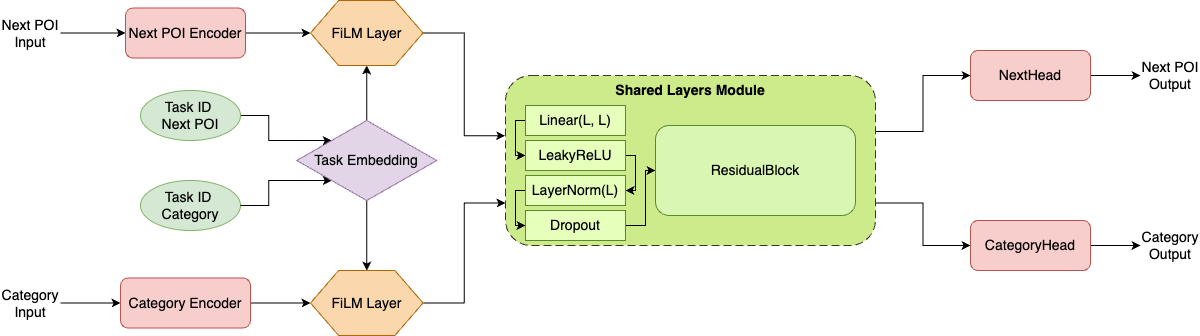
\includegraphics[width=0.92\textwidth]{cbic_mtlnet_arch}
    \end{center}

    \vspace{-1mm}
    {\small
    \begin{itemize}\setlength{\itemsep}{2pt}
        \item \textbf{FiLM:} a learnable task embedding gives a \textbf{scale} and a \textbf{shift} --- both tasks read the same parameters under different scalings.
        \item \textbf{Shared residual blocks} = \textbf{hard parameter sharing} (Def.~2.10). Two disjoint parameter sets: \textbf{shared} $\cdot$ \textbf{task-specific}.
    \end{itemize}\par}

    \vfill
    {\scriptsize\color{secondary}\textbf{Task stamp.} ``Next-POI Prediction'' is the next \textbf{category} (Def.~2.7), not the exact next place. \quad\textbf{Metric stamp.} Chapters 3 and 4 print one F1 \textbf{per category}; Chapter 5 reports \textbf{macro-F1}. Not one scale.\par}
\end{frame}

\subsection{DGI}

% FALA: "O primeiro mecanismo, e ele responde uma pergunta que costuma vir. O DGI roda aqui sobre
% um grafo de Delaunay dos lugares da área, com pesos de aresta que decaem com a distância
% geodésica entre dois lugares, por uma função logarítmica dela. Uma camada de atenção de grafo
% produz um vetor de 64 dimensões por lugar. O objetivo de treino é o infomax da Seção 2:
% distinguir o grafo real de uma versão com as features dos nós embaralhadas, contra um resumo
% global do grafo. Agora o atributo de nó, que é onde eu quero ser exato, porque a nota de rodapé
% do capítulo entregue registra isso. A implementação liberada alimenta a rede com a média dos
% one-hots dos vizinhos do lugar, com o vetor do próprio lugar excluído. A distinção muda como o
% embedding deve ser lido: a entrada descreve a vizinhança, então a tarefa estática que ele
% sustenta é homofilia espacial, e não recuperação do rótulo do próprio lugar. O que sai daí é um
% vetor por lugar. Toda visita àquele lugar entra no modelo com o mesmo vetor, e essa frase é a
% que o Capítulo 5 vai atacar."
\begin{frame}{DGI: how it works $\mid$ why it was used}

    \begin{columns}[t,onlytextwidth]
        \begin{column}{0.48\textwidth}
            \begin{block}{How it works}
                {\small
                \begin{itemize}\setlength{\itemsep}{2pt}
                    \item \textbf{Delaunay graph} over the area's places
                    \item Edge weights decrease with \textbf{geodesic distance}, through a logarithmic function of it
                    \item Graph attention $\rightarrow$ one \textbf{64-dimensional} vector per place
                    \item Infomax objective (Section~2): real graph against shuffled node features, scored on a global summary
                \end{itemize}\par}
            \end{block}
        \end{column}
        \begin{column}{0.48\textwidth}
            \begin{alertblock}{Node features, as released}
                {\small The network is fed \textbf{the mean of the one-hot vectors of a place's graph neighbors, with the place's own vector excluded.}\par}
            \end{alertblock}
            {\small
            \begin{itemize}\setlength{\itemsep}{2pt}
                \item \textbf{Why that matters.} The input describes a \textbf{neighborhood}: \textbf{spatial homophily}, not recall of the place's own label
                \item \textbf{What it gives.} One vector per place --- every visit enters with the same vector
            \end{itemize}\par}
        \end{column}
    \end{columns}
\end{frame}

\subsection{Setup}

% FALA: "O setup em três linhas, e a terceira é a autodeclaração de protocolo que eu prometi na
% Seção 2. Os dados são a Flórida do Gowalla, vinte mil trezentos e um usuários, sessenta e cinco
% mil e nove lugares, novecentos e noventa mil quinhentos e dezoito check-ins, nas mesmas sete
% categorias. As sequências são janelas não sobrepostas de nove visitas, e quem tem menos de cinco
% visitas sai. O protocolo é o estratificado por amostra: cinco partições, uma semente, orçamento
% cheio de épocas, cada tarefa lida na melhor época de validação dela, e média com desvio entre as
% cinco partições. Sem teste de significância. É por isso que este capítulo reporta diferenças, e
% não veredito, e é por isso que eu não vou usar o verbo supera em nenhum slide desta seção."
\begin{frame}{Setup, and the protocol declared}

    \begin{block}{Data and sequences}
        {\small
        Florida, from Gowalla: \textbf{20,301} users, \textbf{65,009} places, \textbf{990,518} check-ins. The seven categories.\\
        Non-overlapping windows of \textbf{nine} visits; users with fewer than \textbf{five} visits are discarded.\par}
    \end{block}
    \begin{alertblock}{Protocol, declared here}
        {\small
        Five-fold cross-validation \textbf{stratified over samples}, one seed $\cdot$ full epoch budget, no early stopping $\cdot$ each task read at \textbf{its own best validation epoch} $\cdot$ mean and standard deviation across the five folds, \textbf{no significance test}.\par}
    \end{alertblock}

    \vfill
    {\centering\textbf{So this chapter reports differences, never a verdict.}\par}
\end{frame}

\subsection{Duas perdas}

% FALA: "Antes de eu nomear o otimizador, o problema que ele existe para resolver. São duas perdas
% e um único conjunto de parâmetros compartilhados, e entre duas soluções não há ordem total: uma
% pode ser melhor numa tarefa e pior na outra, e as duas ficam incomparáveis. Escrever a soma
% ponderada das perdas não remove essa natureza multiobjetivo. Daí vem o vocabulário: uma
% configuração domina outra no sentido de Pareto quando não é pior em nenhuma perda e é melhor em
% pelo menos uma; ela é Pareto-ótima quando nenhuma outra a domina; e o conjunto dos vetores de
% perda dessas configurações é a fronteira de Pareto. A área respondeu a isso com uma família
% inteira de métodos, e a família se divide em duas classes: os que fixam os pesos das perdas e os
% que mudam a direção da atualização. Uma ressalva que é do Capítulo 2 e que eu repito de
% propósito: esta dissertação não reivindica nenhuma propriedade de Pareto para os modelos dela."
\begin{frame}{Two losses, one set of parameters}

    {\small
    \begin{itemize}\setlength{\itemsep}{3pt}
        \item The problem, before any method is named: \textbf{two losses, one set of shared parameters, and no total order between solutions.}
        \item The usual objective is a \textbf{weighted sum} of the task losses. The scalar sum does not remove the multi-objective nature of the problem.
        \item \textbf{Pareto dominance:} no worse on every task loss, better on at least one. \textbf{Pareto optimal:} no other setting dominates it. Their loss vectors form the \textbf{Pareto front}.
        \item Hence a family of methods, in two classes:
        \begin{itemize}
            \item \textbf{set the weights} --- uncertainty weighting, GradNorm, DWA, FAMO
            \item \textbf{change the update direction} --- MGDA, PCGrad, CAGrad, Nash-MTL, Aligned-MTL
        \end{itemize}
    \end{itemize}\par}

    \vfill
    \begin{alertblock}{}
        \centering\textbf{This dissertation claims no Pareto property for its models.}
    \end{alertblock}
\end{frame}

\subsection{Nash-MTL}

% FALA: "O Nash-MTL cai na segunda classe. Ele muda a direção da atualização, tratando a
% combinação dos gradientes como uma barganha cooperativa entre as tarefas: cada tarefa tem uma
% utilidade, que é a redução da perda dela, e a direção escolhida é a que maximiza o produto
% dessas utilidades, o que evita que uma domine a outra. A garantia é convergência para um ponto
% Pareto-estacionário, que é condição necessária e não suficiente para otimalidade de Pareto; a
% otimalidade exigiria uma hipótese de convexidade que uma rede profunda não satisfaz. Agora a
% parte que eu preciso dizer com cuidado. O Capítulo 3 adotou o Nash porque, na comparação dele,
% contra o PCGrad e contra não usar balanceador nenhum, ele deu a menor perda multitarefa
% combinada. Isso é conclusão do tempo dele, enfraquecida depois por um achado sobre a
% implementação do otimizador, e o Capítulo 5 não se apoia nisso. O critério da Seção 2 continua
% de pé: um balanceador só é útil se melhorar sobre uma ponderação fixa bem ajustada."
\begin{frame}{Nash-MTL, and what the chapter may claim about it}

    {\small
    \begin{itemize}\setlength{\itemsep}{3pt}
        \item It \textbf{changes the update direction}: gradient combination as a \textbf{cooperative bargaining problem} among the tasks.
        \item Each task's utility is its own loss reduction; the chosen direction \textbf{maximizes the product of the utilities}, which keeps one task from dominating the other.
        \item Guarantee: a \textbf{Pareto-stationary point} --- necessary, not sufficient, for Pareto optimality, which needs a convexity assumption a deep network does not satisfy.
    \end{itemize}\par}

    \begin{alertblock}{What Chapter 3 claims}
        {\small Against PCGrad and against training without such an optimizer, Nash-MTL gave the lower combined multitask loss, and the chapter adopted it. \textbf{A conclusion of the time}, weakened by a later finding about the optimizer implementation --- and Chapter~5 does not rely on it.\par}
    \end{alertblock}

    {\footnotesize The criterion from Section~2, still standing: \textit{useful only if it improves on a tuned fixed weighting.}\par}
\end{frame}

\subsection{Resultado}

% FALA: "O resultado. Eu prefiro mostrá-lo a afirmá-lo, então são as duas tabelas do capítulo,
% reduzidas ao bloco de F1. À esquerda, a tarefa estática: os nossos dois modelos ficam acima da
% HMRM em todas as categorias. À direita, a tarefa sequencial, e é aqui que está o ponto: as
% lideranças se dividem. O MHA+PE fica com a melhor F1 em Community, Food e Shopping; o nosso
% multitarefa, em Nightlife e Travel; o de tarefa única, em Entertainment e Outdoors. E a
% comparação que interessa é entre as nossas duas colunas, que é a comparação entre multitarefa e
% dedicado. A conclusão é a do próprio capítulo, e está na tela: largamente comparáveis, sem
% vantagem clara ou consistente para o arranjo multitarefa nestes experimentos. Boa parte dessas
% diferenças cai dentro do desvio padrão entre partições. Repito o carimbo, porque ele evita a
% comparação errada mais tarde: isto é F1 por categoria, a convenção dos Capítulos 3 e 4, e não é
% a macro-F1 do Capítulo 5."
\begin{frame}{The null result, shown rather than asserted}

    {\centering\scriptsize F1 block only; mean $\pm$ standard deviation over the five folds.\par}

    \begin{columns}[t,onlytextwidth]
        \begin{column}{0.49\textwidth}
            {\centering\scriptsize\textbf{Static task} --- both of our models score above HMRM in every category\par}
            {\scriptsize
            \setlength{\tabcolsep}{1pt}
            \begin{tabular}{@{}lrrr@{}}
                \toprule
                 & \textbf{MTL} & \textbf{Single} & \textbf{HMRM} \\
                \midrule
                Community     & 52.13 $\pm$ 0.90          & \textbf{53.11 $\pm$ 0.58} & 20.25 $\pm$ 0.52 \\
                Entertainment & 41.44 $\pm$ 1.29          & \textbf{41.73 $\pm$ 1.65} & 13.07 $\pm$ 1.14 \\
                Food          & \textbf{57.43 $\pm$ 1.46} & 56.70 $\pm$ 0.84          & 28.44 $\pm$ 0.42 \\
                Nightlife     & 29.94 $\pm$ 2.27          & \textbf{34.22 $\pm$ 2.08} & 25.54 $\pm$ 1.73 \\
                Outdoors      & 47.19 $\pm$ 1.01          & \textbf{47.75 $\pm$ 0.89} & 16.11 $\pm$ 0.68 \\
                Shopping      & \textbf{62.51 $\pm$ 0.94} & 61.88 $\pm$ 1.01          & 46.69 $\pm$ 0.81 \\
                Travel        & 43.16 $\pm$ 1.43          & \textbf{43.20 $\pm$ 1.94} & 15.25 $\pm$ 1.19 \\
                \bottomrule
            \end{tabular}\par}
        \end{column}
        \begin{column}{0.49\textwidth}
            {\centering\scriptsize\textbf{Next category} --- the leads split\par}
            {\scriptsize
            \setlength{\tabcolsep}{1pt}
            \begin{tabular}{@{}lrrr@{}}
                \toprule
                 & \textbf{MTL} & \textbf{Single} & \textbf{MHA+PE} \\
                \midrule
                Community     & 34.79 $\pm$ 1.05             & \underline{34.90 $\pm$ 0.61} & \textbf{35.83 $\pm$ 1.70} \\
                Entertainment & 24.21 $\pm$ 1.75             & \textbf{26.06 $\pm$ 1.01}    & \underline{25.48 $\pm$ 0.86} \\
                Food          & \underline{28.06 $\pm$ 3.55} & 26.35 $\pm$ 2.97             & \textbf{43.47 $\pm$ 0.50} \\
                Nightlife     & \textbf{22.07 $\pm$ 0.52}    & \underline{21.79 $\pm$ 0.30} & 1.55 $\pm$ 1.50 \\
                Outdoors      & \underline{21.61 $\pm$ 0.50} & \textbf{22.45 $\pm$ 0.81}    & 12.56 $\pm$ 1.94 \\
                Shopping      & \underline{42.58 $\pm$ 2.06} & 42.18 $\pm$ 1.13             & \textbf{43.53 $\pm$ 1.66} \\
                Travel        & \textbf{64.61 $\pm$ 1.11}    & \underline{64.32 $\pm$ 0.88} & 26.91 $\pm$ 0.97 \\
                \bottomrule
            \end{tabular}\par}
        \end{column}
    \end{columns}

    \begin{alertblock}{}
        \centering\scriptsize \textit{``largely comparable, without a clear or consistent advantage for the multitask learning setup in these experiments''}
    \end{alertblock}

    {\scriptsize\color{secondary}\textbf{Task stamp.} the next \textbf{category} (Def.~2.7), not the exact next place. \quad\textbf{Metric stamp.} one F1 \textbf{per category} here; \textbf{macro-F1} in Chapter~5. Not one scale.\par}
\end{frame}

\subsection{Bifurcação}

% FALA: "É aqui que o capítulo deixa de ser um resultado negativo e vira um programa de trabalho,
% porque ele nomeia três suspeitos, e não um. Dissimilaridade das tarefas: o tronco compartilhado
% teria sido forçado a uma representação de compromisso, não especializada para nenhuma das duas.
% Insuficiência da representação: ela não seria rica o bastante para codificar propriedade
% semântica e dinâmica sequencial ao mesmo tempo. Rigidez da topologia: um único bloco
% compartilhado seria restritivo demais. Uma precisão sobre o rodapé, que eu faço questão de
% dizer: a transferência negativa foi hipotetizada aqui, não foi observada."
\begin{frame}{A null with three suspects}

    \begin{block}{1. Task dissimilarity}
        {\footnotesize A static task and a sequential task may force the shared trunk into a \textbf{compromise representation}, specialized for neither.\par}
    \end{block}
    \vspace{-2mm}
    \begin{block}{2. Representation insufficiency}
        {\footnotesize The shared representation may not be rich enough to encode \textbf{semantic properties and sequential dynamics at once}.\par}
    \end{block}
    \vspace{-2mm}
    \begin{block}{3. Topology rigidity}
        {\footnotesize One shared block may be too restrictive; \textbf{soft sharing or expert-based routing} might fit better.\par}
    \end{block}

    \vfill
    {\centering\textbf{Negative transfer was hypothesized here. It was never observed.}\par}
\end{frame}

\subsection{Transição interna}

% FALA: "Um nulo com três suspeitos não encerra a investigação: ele desenha o próximo experimento.
% Congelar a arquitetura e mover apenas a entrada."
{
\specialframe
\begin{frame}
    \vfill
    \begin{center}
        {\large A null with three suspects does not close the investigation.\\[1mm]
        It designs the next experiment:}

        \bigskip
        {\Large\bfseries keep the architecture fixed, and move only the input.}
    \end{center}
    \vfill
\end{frame}
}

\section[ST-MTLNet]{ST-MTLNet: Spatio-Temporal POI Representations}

% ============================================================
% SEÇÃO 4 · Capítulo 4 --- CoUrb 2026
% ============================================================

\subsection{Pergunta herdada}

% FALA: "O segundo estudo pega a pergunta herdada e a transforma em experimento controlado. O
% gargalo é a representação, ou é a topologia de compartilhamento? Para separar as duas, ele
% mantém o MTLnet sem alterar uma linha: o mesmo tronco, a mesma modulação FiLM, o mesmo
% balanceador de gradientes, os mesmos hiperparâmetros. Só a entrada se move. A entrada antiga é o
% embedding monolítico de 64 dimensões do DGI. A entrada nova é a concatenação de três
% codificadores independentes, um espacial, um temporal e um categórico, de 64 dimensões cada, o
% que dá 192. E os encoders de tarefa projetam qualquer entrada para a mesma largura latente de
% 256 nos dois braços. É esse congelamento que faz o resultado ser diagnóstico, e não apenas
% melhor."
% (Esta fala de 40 s cobre este frame E o frame seguinte, o da Fig. 2.)
\begin{frame}{Architecture or representation?}

    \begin{alertblock}{The inherited question --- suspect 2 against suspect 3}
        \centering Is the bottleneck the \textbf{representation}, or the \textbf{sharing topology}?
    \end{alertblock}

    {\small
    \begin{itemize}\setlength{\itemsep}{3pt}
        \item \textbf{The design that separates them:} MTLnet is kept unchanged, and \textbf{only the input moves}. Same trunk, same FiLM, same balancer, same hyperparameters.
        \item \textbf{Old input:} one monolithic \textbf{64-dimensional} place embedding (DGI).
        \item \textbf{New input:} three independent \textbf{64-dimensional} encoders --- spatial, temporal and categorical --- concatenated into \textbf{192}.
        \item Same latent width on both sides: the per-task encoders project any input to \textbf{256}.
        \item Three states: Florida, California, Texas. Protocol as in Chapter~3.
    \end{itemize}\par}

    \vfill
    {\scriptsize\color{secondary}\textbf{Task stamp.} ``Next-POI Prediction'' is the next \textbf{category} (Def.~2.7), not the exact next place.\par}
\end{frame}

% FALA: (este frame não tem fala própria --- é a arte da Fig. 2, falada dentro dos 40 s do slide
% anterior, "Architecture or representation?".)
\begin{frame}{Architecture or representation?}

    \framesubtitle{The same MTLnet, with the decomposed input in place of the monolithic one}

    \begin{center}
        
\includegraphics[width=\textwidth]{arquitetura_modelo}
    \end{center}

    \vfill
    {\scriptsize\color{secondary}\textbf{Task stamp.} ``Next-POI Prediction'' is the next \textbf{category} (Def.~2.7), not the exact next place. \quad\textbf{Metric stamp.} Chapters 3 and 4 print one F1 \textbf{per category}; Chapter 5 reports \textbf{macro-F1}. Not one scale.\par}
\end{frame}

\subsection{HGI}

% FALA: "O segundo mecanismo. É o conceito que sustenta o resto da dissertação, então eu vou com
% calma. O HGI monta uma hierarquia de três níveis: lugar, região, cidade. Um codificador de
% categoria pré-treinado dá as features iniciais dos lugares; uma camada de convolução sobre um
% grafo de Delaunay da área acrescenta contexto espacial a cada um; uma atenção multi-cabeça
% agrega os embeddings dos lugares de uma região; e uma soma ponderada por área sobre as regiões
% produz um embedding de cidade. O que se maximiza é a informação mútua entre dois níveis
% adjacentes dessa hierarquia. A peça que faz isso é um discriminador bilinear, que combina dois
% embeddings por uma matriz aprendida e passa o resultado por uma função logística, e a perda
% premia pontuação alta para um par verdadeiro e baixa para um par falso. Nenhum rótulo de tarefa
% final entra nessa comparação. Há uma consequência do desenho que vai importar duas vezes mais
% adiante. O treino atualiza junto o codificador de lugar, a agregação e o codificador de região,
% e a pertinência a região ainda entra pelos pesos das arestas. Então a saída no nível de lugar
% não descreve o lugar isolado: ela já reflete a região a que o lugar pertence. E um limite que eu
% declaro junto: o HGI foi desenvolvido e avaliado para representação de região urbana, e esta
% dissertação reaproveita a saída de nível de lugar para predição sequencial, um uso que a
% avaliação original não cobre."
\begin{frame}{HGI: how it works $\mid$ why it was used}

    \begin{columns}[t,onlytextwidth]
        \begin{column}{0.48\textwidth}
            \begin{block}{How it works, in order}
                {\footnotesize Pretrained category encoder $\rightarrow$ one \textbf{graph convolution} over a Delaunay graph $\rightarrow$ \textbf{multi-head attention} over a region's places $\rightarrow$ \textbf{area-weighted sum} over regions $\rightarrow$ one city embedding.\par}
            \end{block}
            \vspace{-2mm}
            \begin{block}{What is maximized}
                {\footnotesize Mutual information between \textbf{two adjacent levels}, through a \textbf{bilinear discriminator}. \textbf{No label of any downstream task enters that comparison.}\par}
            \end{block}
        \end{column}
        \begin{column}{0.48\textwidth}
            \begin{alertblock}{A consequence of the design}
                {\footnotesize Place encoder, aggregation and region encoder are updated together, and region membership also enters through the edge weights. \textbf{The place-level output already reflects the region the place belongs to.}\par}
            \end{alertblock}
            \vspace{-3mm}
            \begin{block}{Why it is used here --- and the limit}
                {\footnotesize Built for \textbf{urban region representation}; its \textbf{place-level} output is repurposed here for sequential prediction --- \textbf{a use the original evaluation does not cover}.\par}
            \end{block}
        \end{column}
    \end{columns}
\end{frame}

\subsection{Codificadores}

% FALA: "Por que estes codificadores, e não outros quaisquer. O canal espacial existe porque o
% MTLnet codificava espaço só implicitamente, pela topologia do grafo, e nunca como coordenada
% contínua. O estudo compara dois com hipóteses diferentes: o SIREN, que modela uma função
% contínua das coordenadas normalizadas com ativações senoidais, e o Sphere2Vec-M, que é
% multiescala e opera direto em coordenadas esféricas, preservando propriedades de distância
% geodésica. Os dois são treinados com a mesma perda contrastiva sobre distância geográfica, com
% par abaixo de dez quilômetros como positivo e acima de setenta como negativo, e é isso que faz a
% comparação isolar a arquitetura. O canal temporal existe porque o MTLnet não tinha representação
% temporal nenhuma, e o Time2Vec combina um termo linear, de tendência global, com termos
% senoidais, para os padrões cíclicos de hora do dia e dia da semana. O canal categórico existe
% porque o DGI codificava categoria pela estrutura do grafo, sem capturar relação hierárquica ou
% regional entre elas, e ele vem em duas fases. Primeiro um codificador de lugar, que aprende
% coocorrência entre categorias a partir de caminhadas aleatórias sobre o grafo espacial, com
% amostragem negativa e um termo que amarra cada classe fina à categoria de topo dela. Depois o
% HGI, que acrescenta a hierarquia regional sobre esse resultado."
\begin{frame}{Why these encoders}

    \begin{columns}[t,onlytextwidth]
        \begin{column}{0.44\textwidth}
            \begin{block}{Spatial, 64 d}
                {\footnotesize
                \textbf{Why:} space was encoded only through graph topology, never as a continuous coordinate.
                \begin{itemize}\setlength{\itemsep}{1pt}
                    \item \textbf{SIREN} --- sinusoidal activations over normalized coordinates
                    \item \textbf{Sphere2Vec-M} --- multi-scale, spherical coordinates, geodesic distance preserved
                    \item One contrastive loss for both: positive under \textbf{10 km}, negative over \textbf{70 km}
                \end{itemize}\par}
            \end{block}
        \end{column}
        \begin{column}{0.52\textwidth}
            \begin{block}{Temporal, 64 d}
                {\footnotesize
                \textbf{Why:} no explicit temporal representation.\\
                \textbf{Time2Vec} --- a linear term for global trend, sinusoidal terms for hour of day and day of week.\par}
            \end{block}
            \vspace{-3mm}
            \begin{block}{Categorical, 64 d, two phases}
                {\footnotesize
                \textbf{Why:} graph structure alone --- no hierarchy, no region.\\
                \textbf{1. POI Encoder} (a category encoder trained on random walks) --- skip-gram with negative sampling; each \textbf{fine class} tied to its top-level category.\\
                \textbf{2. HGI} --- the regional hierarchy above.\par}
            \end{block}
        \end{column}
    \end{columns}
\end{frame}

\subsection{Ressalva da tarefa estática}

% FALA: "Aqui a ordem importa mais que o número, então eu digo a ressalva primeiro, em uma
% cláusula, e sigo em frente. Depois da publicação, nós estabelecemos que a entrada da tarefa
% estática deste capítulo contém o rótulo que ela prevê: a feature de tipo de local mapeia
% um-para-um nas sete categorias de topo. A acurácia reportada nessa tarefa mede essa consulta, e
% não inferência semântica aprendida. A consequência é direta e eu prefiro dizê-la eu mesmo: o
% ganho estático não diz nada sobre a tarefa sequencial. Dito isso, o número. Na tarefa estática a
% entrada decomposta lidera nas vinte e uma combinações de categoria e estado, com ganhos médios
% por estado de vinte vírgula dois a vinte e dois pontos percentuais. E eu declaro o que essa
% faixa é: é o melhor dos dois codificadores espaciais em cada combinação, não é nenhum dos dois
% sozinho."
\begin{frame}{The caveat, then the number}

    \begin{alertblock}{From the chapter preface}
        {\small After publication, we established that the input to this chapter's static task contains the label it predicts: the venue-type feature maps one-to-one onto the seven top-level categories across the Gowalla state subsets used, so the reported static-task accuracy measures that lookup rather than learned semantic inference.\par}
    \end{alertblock}

    {\small
    \begin{itemize}\setlength{\itemsep}{3pt}
        \item<1-> \textbf{The static gain therefore says nothing about the sequential task.}
        \item<2-> Then, and only then: the decomposed input leads in \textbf{all 21 category-state combinations}, with average gains per state of \textbf{20.2 to 22.0 percentage points}.
        \item<2-> \textbf{Declared with the range:} it is the \textbf{better of the two spatial encoders in each combination}, not either encoder on its own.
    \end{itemize}\par}

    \vfill
    {\scriptsize\color{secondary}\textbf{Metric stamp.} Chapters 3 and 4 print one F1 \textbf{per category}; Chapter 5 reports \textbf{macro-F1}. Not one scale.\par}
\end{frame}

\subsection{Resultado diagnóstico}

% FALA: "Agora a tarefa que produz o diagnóstico, que é a sequencial, e a razão é uma só: o alvo
% dela nunca está na entrada. Na tela está a Flórida, com os três modelos lado a lado; Califórnia
% e Texas eu tenho prontos se a banca quiser. O cenário aqui é mais heterogêneo do que na tarefa
% estática, e continua favorável à entrada decomposta. Contando o melhor dos dois codificadores
% espaciais por combinação, os modelos espaço-temporais ficam com a média mais alta em quinze das
% vinte e uma combinações de categoria e estado, e o MTLnet, com a entrada original, retém seis.
% Uma dessas seis o capítulo chama, nas palavras dele, de um empate técnico adicional: é Outdoors
% na Flórida, onde a média do MTLnet fica dois centésimos de ponto percentual acima da melhor
% variante, dentro de um desvio padrão. Os maiores ganhos estão em Food, em que as duas variantes
% ficam acima nos três estados, com melhoria consistente também em Shopping e Community. E o
% carimbo de novo: isto é F1 por categoria, não é macro-F1."
\begin{frame}{The diagnostic result is the sequential task}

    \framesubtitle{Table 7, Florida --- the sequential target is never in the input}

    \begin{columns}[T,onlytextwidth]
        \begin{column}{0.57\textwidth}
            {\scriptsize
            \setlength{\tabcolsep}{2pt}
            \begin{tabular}{@{}lccc@{}}
                \toprule
                 & \textbf{MTLnet} & \textbf{ST-MTLNet} & \textbf{ST-MTLNet} \\
                 &                 & \textbf{SIREN}     & \textbf{Sphere2Vec-M} \\
                \midrule
                Community     & 34.33 $\pm$ 1.33          & \textbf{38.31 $\pm$ 0.90} & 37.98 $\pm$ 1.22 \\
                Entertainment & 25.34 $\pm$ 1.07          & \textbf{31.38 $\pm$ 1.72} & 31.24 $\pm$ 2.41 \\
                Food          & 27.12 $\pm$ 2.79          & \textbf{41.91 $\pm$ 1.93} & 41.65 $\pm$ 3.15 \\
                Nightlife     & 21.33 $\pm$ 1.61          & 23.32 $\pm$ 2.74          & \textbf{23.98 $\pm$ 1.94} \\
                Outdoors      & \textbf{21.61 $\pm$ 0.99} & 21.29 $\pm$ 1.59          & 21.59 $\pm$ 1.91 \\
                Shopping      & 39.62 $\pm$ 3.40          & 44.00 $\pm$ 2.04          & \textbf{44.66 $\pm$ 2.38} \\
                Travel        & \textbf{64.47 $\pm$ 1.02} & 45.00 $\pm$ 1.10          & 44.93 $\pm$ 1.11 \\
                \bottomrule
            \end{tabular}\par}
        \end{column}
        \begin{column}{0.41\textwidth}
            {\scriptsize
            \begin{itemize}\setlength{\itemsep}{3pt}
                \item Over the three states, the decomposed input holds the higher mean in \textbf{15 of the 21} category-state combinations
                \item \textbf{MTLnet, with its original input, retains six} --- one of them \textit{``one additional technical tie''}, at \textbf{Outdoors} in Florida, where the MTLnet mean is higher than the best variant by \textbf{0.02 percentage points}, inside one standard deviation
                \item Gains concentrate at \textbf{Food}, in all three states; also \textbf{Shopping} and \textbf{Community}
            \end{itemize}\par}
        \end{column}
    \end{columns}

    \vfill
    {\scriptsize\color{secondary}\textbf{Task stamp.} the next \textbf{category} (Def.~2.7), not the exact next place. \quad\textbf{Metric stamp.} one F1 \textbf{per category} here; \textbf{macro-F1} in Chapter~5. Not one scale.\par}
\end{frame}

\subsection{Bordas honestas}

% FALA: "Três limites, e eu ofereço os três antes que me peçam. O primeiro é o Travel, e ele
% precisa de rótulo de tarefa, senão a sala se confunde: Travel na classificação de categoria
% melhora, Travel na próxima categoria não. Na tarefa sequencial o MTLnet mantém a liderança na
% Flórida e na Califórnia, e a razão está escrita no capítulo: movimento de longa distância é
% esparso, e a topologia de grafo preserva relação entre lugares geograficamente distantes melhor
% do que um codificador baseado em coordenada. O segundo limite é que não existe codificador
% espacial universalmente melhor. O SIREN se destaca mais na Flórida e na Califórnia, o
% Sphere2Vec-M no Texas, e a adequação depende de como os lugares se distribuem em cada
% território. O terceiro é o que eu esperaria que a banca perguntasse, então eu digo primeiro: a
% comparação não é pareada em largura. São 192 dimensões contra 64. O capítulo declara isso como
% limite e pede um controle de dimensão equalizada, e eu não vou defender o ponto: parte do ganho
% pode vir da largura. Junto com isso, os três componentes entram sempre juntos, então este
% capítulo não isola a contribuição de cada codificador."
\begin{frame}{What the decomposition moved, and where it did not}

    \begin{block}{Travel, labeled by task}
        {\footnotesize
        \textit{Travel (category classification)} \textcolor{primary}{\textbf{moved}} $\;\cdot\;$ \textit{Travel (next category)} \textcolor{alert}{\textbf{did not}}.\\
        On the sequential task MTLnet keeps the lead at \textbf{Florida} and \textbf{California}: long-distance movement is sparse, and graph topology preserves relationships between geographically distant places better than a coordinate-based encoder does.\par}
    \end{block}
    \begin{columns}[t,onlytextwidth]
        \begin{column}{0.48\textwidth}
            \begin{block}{No universally better spatial encoder}
                {\footnotesize \textbf{SIREN} leads more often at Florida and California, \textbf{Sphere2Vec-M} at Texas. Suitability depends on how the places are distributed over each territory.\par}
            \end{block}
        \end{column}
        \begin{column}{0.48\textwidth}
            \begin{alertblock}{The comparison is not width-matched}
                {\footnotesize \textbf{192 dimensions against 64.} The chapter states this as a limit and asks for an equal-dimension control.\par}
            \end{alertblock}
        \end{column}
    \end{columns}

    \vfill
    {\footnotesize \textit{The three components are used together, so this chapter does not isolate the contribution of each encoder.}\par}
\end{frame}

\subsection{Entrega}

% FALA: "Com a arquitetura fixa, a entrada moveu o resultado: a representação é o gargalo. Mas o
% diagnóstico ainda é em nível de lugar, sob um protocolo que deixa o mesmo usuário dos dois lados
% da divisão. O terceiro estudo reconstrói as três camadas: representação, topologia e protocolo."
{
\specialframe
\begin{frame}
    \vfill
    \begin{center}
        {\large\bfseries With the architecture fixed, the input moved the result:\\[1mm]
        the representation is the bottleneck.}

        \bigskip
        {\normalsize The diagnosis is still at the place level, under a protocol that leaves the same user on both sides of the split.}

        \bigskip
        {\large The third study rebuilds three layers:\\[1mm]
        \textbf{representation $\cdot$ topology $\cdot$ protocol.}}
    \end{center}
    \vfill
\end{frame}
}

\section[Check2HGI]{A Check-in-Level Multitask Study of Next Category and Region}

% ============================================================
% SEÇÃO 5 · Capítulo 5 --- MobiWac 2026: a resolução — 20 min (PLANO §3, Seção 5)
% Proveniência no divisor: MobiWac 2026, submitted, under review. Vitor H. O. Silva, first author.
% Ordem fixa (PLANO §3): 5.1 · 5.2A · 5.2 · 5.3 · 5.4 · 5.5 · 5.6.
% ============================================================

\subsection{O que muda}

% FALA: As três mudanças do último estudo, e nenhuma delas é preferência minha: as três são consequência do diagnóstico do capítulo anterior.
% A representação sai do nível de lugar para o nível de check-in, porque um vetor por lugar não distingue um almoço de quarta-feira de uma noite de sábado no mesmo lugar.
% A topologia sai do compartilhamento rígido para atenção cruzada entre fluxos por tarefa, com um caminho espacial privado na saída de região.
% E o protocolo sai do estratificado por amostra para validação cruzada com **usuários disjuntos**, quatro sementes, e testes fixados antes de qualquer resultado ser lido.
% Aqui eu cumpro o aviso que dei na Seção 2: **o par de tarefas muda**.
% Com uma entrada por visita, a classificação estática vira um par pouco natural, e o par passa a ser próxima categoria mais próxima região, dois alvos finais sequenciais.
% A restrição da abertura continua valendo: um artefato, uma passagem, duas respostas.
\begin{frame}{Three changes, each a consequence of the diagnosis}
    \framesubtitle{Not a preference --- each follows from the previous chapter}

    {\small
    \setlength{\tabcolsep}{4pt}
    \begin{tabular}{@{}l l l@{}}
        \toprule
                                & \textbf{From $\rightarrow$ To}                     & \textbf{Why}                          \\
        \midrule
        \textbf{Representation} & place level $\rightarrow$ \alert{check-in level}   & weekday lunch $\neq$ Saturday night   \\
        \textbf{Topology}       & hard parameter sharing $\rightarrow$ \alert{cross-attention} & private spatial path for region \\
        \textbf{Protocol}       & sample-stratified $\rightarrow$ \alert{user-disjoint} & four seeds, tests fixed in advance \\
        \bottomrule
    \end{tabular}}

    \medskip
    \begin{alertblock}{The task pair changes here}
        \small
        Under a check-in-level representation, static category classification is a less natural
        companion than a second sequential target: the pair becomes
        \textbf{next category $+$ next region}.
        \smallskip

        The restriction holds: \textbf{one artifact, one forward pass, two answers.}
    \end{alertblock}
\end{frame}

\subsection{Trabalhos relacionados deste estudo}

% FALA: Trabalho relacionado deste estudo, que os dois primeiros não têm, e a primeira metade é a tarefa nova.
% Próxima região é classificação sobre as regiões candidatas do conjunto, de 520 classes em Istambul a 8.501 na Califórnia:
% mais grossa que lugar não quer dizer mais fácil.
% Prever sobre uma partição do mapa é a formulação padrão em mobilidade, com célula de grade como alvo;
% aqui entra no lugar dela a unidade administrativa de bairro.
% E onde a área já modela várias granularidades, categoria e região aparecem como sinais auxiliares de um alvo principal de próximo lugar.
% Eu estudo o par como objeto. O escopo vai junto com a motivação: preparação em nível de bairro, e nenhum serviço construído ou avaliado aqui.
\begin{frame}{Next region: the task, and why it is worth predicting}
    \framesubtitle{Related work of this study, part 1 of 2}

    \small
    \begin{itemize}
        \item \textbf{The task.} Classification over the dataset's candidate regions ---
              \alert{520 classes (Istanbul) to 8,501 (California)}. Coarser than a place, and not easier.
        \item \textbf{Why this target.} The category says \emph{what type} of place comes next;
              the region says \emph{where}, hence where to prepare.
        \item \textbf{Where it sits.} The standard mobility formulation targets a \textbf{grid cell};
              this task substitutes official neighborhood-scale units. In MCMG and HMT-GRN,
              category and region are \textbf{auxiliary signals} for a primary next-place task.
        \item \textbf{Scope, stated with the motivation.} Neighborhood-level preparation:
              demand and load anticipation, caching ahead of time, capacity planning.
              \emph{A census tract is a neighborhood, not a radio cell.}
              \alert{No such service is built or evaluated here.}
    \end{itemize}
\end{frame}

% FALA: Segunda metade: por que uma representação por visita é nova nesta linha.
% A arte prévia mais próxima é o CTLE, que também dá um vetor por visita, aprendido mascarando e reconstruindo partes da sequência de check-ins do usuário.
% A diferença é de construção. O CTLE é um modelo de sequência, um Transformer que lê a própria sequência;
% o Check2HGI continua um modelo de grafo, com a mesma hierarquia de lugar, região e cidade e o mesmo objetivo infomax, agora um nível mais fundo.
% E o CTLE pré-treina só sobre identificador de lugar e marca de tempo, então o vocabulário de categoria nunca entra no treino dele.
% A novidade que eu reivindico é a combinação.
\begin{frame}{Why a per-visit representation is new in this line}
    \framesubtitle{Related work of this study, part 2 of 2}

    \small
    \begin{itemize}
        \item \textbf{CTLE} --- the closest prior contextual check-in representation:
              one vector per visit, learned by masking and reconstructing parts of a user's
              check-in sequence.
        \item \textbf{The difference is the construction.} CTLE is a \textbf{sequence model},
              a Transformer over the check-in sequence. Check2HGI stays a \textbf{graph model}:
              same place, region, city hierarchy, same infomax objective, extended one level deeper.
        \item \textbf{What CTLE pretrains on:} place identifiers and timestamps alone ---
              the category vocabulary never enters its training.
    \end{itemize}

    \begin{block}{}
        \small \alert{The novelty is the combination:} per-visit context \textbf{inside} a
        hierarchical graph-infomax representation.
    \end{block}
\end{frame}

\subsection{A representação}

% FALA: O Check2HGI, e ele se apoia direto no HGI do capítulo anterior. O HGI tinha três níveis: lugar, região e cidade.
% O Check2HGI acrescenta **um quarto nível abaixo do lugar**, que é o próprio check-in.
% As arestas ligam cada nível ao de cima, ligam lugares próximos no nível de lugar, e ligam os check-ins consecutivos de um mesmo usuário, com um peso que decai conforme o intervalo entre as visitas cresce.
% Duas visitas ao mesmo lugar se encontram pelo nó de lugar, um nível acima. O treino é o objetivo infomax da Seção 2, agora um nível mais fundo:
% cada vetor aprende a reconhecer a vizinhança verdadeira e a rejeitar uma embaralhada.
% Junto com ele vão dois termos auxiliares pequenos, de pesos 0,3 e 0,1, e nenhum dos dois usa rótulo.
% Este é o ponto que eu quero deixar assentado antes de qualquer resultado: **o grafo nunca vê a próxima categoria nem a próxima região**.
% E do grafo treinado saem duas tabelas: um vetor de 64 dimensões por visita, e um vetor por região.
% São essas duas tabelas que o modelo da próxima tela vai ler.
\begin{frame}{Check2HGI: a fourth level below the place}
    \centering
    
\includegraphics[width=0.50\textwidth]{fig1_dataflow}

    \raggedright
    \small
    \begin{itemize}
        \item \textbf{Four levels:} check-in $\cdot$ place $\cdot$ region $\cdot$ city ---
              \alert{the check-in is the new level}
        \item \textbf{Edges:} to the level above $\cdot$ nearby places $\cdot$ a user's consecutive
              check-ins, weight decaying as the time gap grows
        \item \textbf{No task label:} infomax (real neighborhood against a shuffled one) $+$ two
              label-free auxiliary terms (0.3 and 0.1)
        \item \textbf{Two outputs:} one 64-dimensional vector per visit $\cdot$ one vector per region
    \end{itemize}
\end{frame}

% FALA: O que cada visita contribui na entrada, e é aqui que está a informação que um vetor por lugar não consegue carregar. Três grupos. O semântico:
% a categoria do lugar visitado, como indicador sobre as classes. O tempo cíclico:
% hora do dia e dia da semana pelo seno e pelo cosseno, para que o fim e o começo de cada ciclo fiquem vizinhos, e não em pontas opostas de uma escala.
% E os tempos decorridos:
% o intervalo desde a visita anterior e o intervalo desde a primeira visita daquele usuário, os dois comprimidos por logaritmo, mais o intervalo dentro do mesmo dia e um indicador de primeira visita.
% É isso que dá ritmo à representação: distinguir a visita que vem minutos depois da anterior daquela que abre um passeio novo.
% E aqui um princípio de projeto, na redação do próprio capítulo:
% as arestas entre visitas consecutivas correm numa direção só, da visita anterior para a posterior. A razão está na mesma frase:
% o alvo é predito do passado do usuário, então a representação é construída só do passado. Todo valor é medido até a própria visita.
\begin{frame}{What each visit contributes}
    \framesubtitle{The node features, and one design principle}

    \small
    \begin{itemize}
        \item \textbf{Semantic.} The category of the visited place, as an indicator over the classes.
        \item \textbf{Cyclical time.} Time of day and day of week, through their sine and cosine ---
              the endpoints of the daily and weekly cycles fall next to each other.
        \item \textbf{Elapsed time.} Time since the user's previous visit and since the user's first
              visit, both log-compressed; the gap within the same calendar day; a first-visit
              indicator. \emph{These give the representation a sense of tempo.}
    \end{itemize}

    \begin{alertblock}{A design principle, in the chapter's own wording}
        \small
        \emph{The consecutive-visit edges run in one direction only, from an earlier visit to a
        later one, for the same reason: a target is predicted from a user's past, so the
        representation is built from the past alone.}
    \end{alertblock}

    {\scriptsize Every value is measured up to the visit itself: a node describes the visit and the
    history preceding it, never anything that follows.\par}
\end{frame}

% FALA: E este é o resultado da representação sozinha, antes de qualquer modelo. A pergunta é simples: esses vetores por visita separam as sete categorias?
% A silhueta por categoria mede quão compactos e quão separados estão os grupos rotulados, numa escala de menos um a um.
% Ela dá cerca de **0,57** para a representação em nível de check-in contra cerca de **0,00** para o embedding por lugar.
% A pureza de categoria dos dez vizinhos mais próximos dá cerca de **0,98** contra **0,78**. As duas médias são sobre os cinco estados americanos.
% Duas ressalvas, e eu faço as duas antes de alguém pedir. A primeira:
% a figura caracteriza a **família** da representação, e não a configuração exata que eu avalio depois.
% É por isso que ela não precisa de partição, de semente nem de pareamento, e é por isso que ela pode vir antes do protocolo. A segunda:
% a mesma geometria **não** separa regiões. O benefício é de categoria, e o fluxo espacial do modelo lê os vetores de região do mesmo grafo, não estes.
% Nenhum p-valor nesta tela: aqui é geometria, e o teste vem depois, no bloco de resultados.
\begin{frame}{The geometry of the vectors}
    \centering
    
\includegraphics[width=0.47\textwidth]{fig3_embquality}

    \raggedright
    \small
    \begin{itemize}
        \item \textbf{Silhouette by category} (how tight and well separated the seven labeled groups
              are, $-1$ to $1$): \alert{about 0.57} check-in level against \textbf{about 0.00} place
              embedding
        \item \textbf{Nearest-neighbor category purity} ($k = 10$): \alert{about 0.98} against
              \textbf{about 0.78}. Both averaged over the five U.S. states.
    \end{itemize}

    {\scriptsize
    \emph{These measures characterize the representation family, not the exact configuration
    evaluated later. They need no fold, no seed, and no pairing.}\par
    \emph{The same geometry does not separate regions. The benefit is category-only; the model's
    spatial stream reads the region-level vectors of the same graph instead.}\par}
\end{frame}

\subsection{A arquitetura}

% FALA: A arquitetura, e o que mudou no multitarefa. Cada tarefa tem a sua entrada.
% A de categoria lê a janela de vetores por visita, que é o fluxo semântico.
% A de região lê a mesma janela de visitas, só que cada visita agora representada pelo vetor treinado do nó de região dela, que é o fluxo espacial.
% As duas passam por encoders privados, sem peso nenhum compartilhado. E o tronco compartilhado é uma pilha de dois blocos de atenção cruzada:
% em cada bloco a atenção deixa um fluxo ler as features do outro, enquanto cada um mantém os próprios pesos feed-forward.
% É esta a frase que eu quero que fique da tela:
% as tarefas compartilham **por troca de informação entre fluxos por tarefa**, e não por possuírem camadas ocultas em comum.
% Comparem com o Capítulo 3, onde tudo atravessava um tronco único e as tarefas só se separavam nas saídas.
% É a mesma família de modelos, com a topologia de compartilhamento trocada, e a topologia era um dos três suspeitos do nulo.
\begin{frame}{The architecture: sharing by exchange}
    \framesubtitle{Two inputs, one model}

    \begin{columns}[T]
        \begin{column}{0.40\textwidth}
            \centering
            
\includegraphics[width=0.95\linewidth]{fig2_model}
        \end{column}
        \begin{column}{0.58\textwidth}
            \footnotesize
            \begin{itemize}
                \item \textbf{Two inputs, one model.} The category task reads the window of
                      per-visit vectors (\textbf{semantic stream}); the region task reads the same
                      window, each visit now represented by the trained vector of its region node
                      (\textbf{spatial stream}).
                \item \textbf{Private per-task encoders} --- a small input network per task, with no
                      shared weights.
                \item \textbf{The shared trunk:} a cross-attention stack of two blocks. Attention
                      lets each stream read the other's features, while each keeps its own
                      feed-forward weights.
            \end{itemize}
        \end{column}
    \end{columns}

    \begin{alertblock}{}
        \footnotesize
        The tasks share by \textbf{exchanging information between per-task streams}, not by owning
        hidden layers in common.
    \end{alertblock}
\end{frame}

% FALA: Duas coisas fecham a arquitetura, e depois uma posição que eu preciso enunciar com precisão. A primeira é o caminho espacial privado:
% a saída de região tem, além do tronco, um ramo pequeno **dentro do mesmo modelo**, e não um segundo modelo, que lê a janela espacial e contorna o tronco.
% A tarefa de categoria não toca nesse ramo. A segunda é a perda:
% uma soma de peso fixo, meio a meio entre as duas tarefas, e o peso é fixo **de propósito**, para que qualquer melhora sobre os dedicados venha da representação compartilhada e não de um esquema adaptativo de ponderação.
% A saída de categoria treina com ajuste de logit, que empurra a fronteira de decisão para o posterior balanceado que a macro-F1 premia, e o **modelo dedicado de categoria recebe o mesmo ajuste**, então a comparação entre os dois não é afetada por ele.
% Agora a posição. A evidência aqui **não separa** as contribuições do tronco compartilhado e do caminho espacial privado.
% Ela não estabelece que o compartilhamento ajuda, e não o descarta. A afirmação que eu faço é sobre o desenho:
% esta combinação produz uma saída de região acima de dois modelos dedicados, nos dois conjuntos com os maiores números de regiões.
% Não é uma afirmação sobre transferência entre tarefas.
\begin{frame}{The private spatial path, and what the evidence does not separate}
    \footnotesize
    \begin{itemize}
        \item \textbf{The private spatial path.} A small branch \emph{inside the one model}, not a
              second model: it reads the spatial input window, bypasses the shared trunk, and feeds
              the region output only. \alert{The category task does not touch this branch.}
        \item \textbf{The training loss:} a fixed-weight sum, \textbf{0.5 category $+$ 0.5 region}.
              Fixed by design, so that any improvement over the dedicated models comes from the
              shared representation and not from an adaptive weighting scheme.
        \item \textbf{The category output is trained with logit adjustment} ($\tau = 0.5$, training
              only; inference uses the unadjusted logits), which shifts the decision boundary toward
              the balanced posterior that macro-F1 rewards. \alert{The dedicated category model
              receives the same adjustment}, so the comparison is not affected by it.
              Class weighting was tested on both outputs and lowered both scores.
    \end{itemize}

    \begin{alertblock}{The position on the shared trunk}
        \scriptsize
        \emph{The evidence does not separate the contributions of the shared trunk and the private
        spatial path. It does not establish that sharing helps, and it does not rule it out.
        The claim I make is about the design.}
    \end{alertblock}
\end{frame}

\subsection{O protocolo}

% FALA: O protocolo, e ele é o degrau que sustenta tudo o que vem depois. São quatro passos, e cada um responde a uma pergunta que o anterior deixa aberta.
% Primeiro passo: qual é a unidade de dados. Validação cruzada de cinco partições, **disjunta por usuário**:
% todas as janelas de um usuário ficam na mesma partição, então as visitas de um usuário de teste nunca aparecem no treino.
% Isto é exatamente a reparação da limitação que eu declarei no Capítulo 3.
% A estratificação é pelo rótulo da próxima categoria, porque as sete classes são desbalanceadas. As janelas são **sobrepostas, de passo um**:
% para cada usuário com pelo menos dez visitas, começa uma janela de nove visitas em cada visita, e a visita seguinte é o alvo;
% janelas curtas duplicadas, que terminam no mesmo alvo, são removidas. Repito o aviso da Seção 2:
% **estas não são as mesmas janelas** dos Capítulos 3 e 4, que usaram janelas não sobrepostas.
% E uma coisa que eu digo agora para não parecer descoberta depois:
% a partição retida é também a de validação, não há um terceiro corte, e é daí que sai o segundo dos meus limites.
\begin{frame}{The protocol, in four steps}
    \framesubtitle{1 $\cdot$ the unit of data}

    \small
    \begin{itemize}
        \item \textbf{User-disjoint five-fold cross-validation.} All windows from one user stay in
              the same fold, so a test user's visits never appear in training.
              \alert{This is the repair of the limitation declared in Chapter 3.}
        \item Stratified by the \textbf{next-category label}, because the seven classes are imbalanced.
        \item \textbf{Sliding windows, stride 1.} For each user with at least ten visits, a window of
              nine visits starts at each visit and the next visit is the target; duplicated short
              padded windows ending at the same target are removed.
        \item \alert{Not the same windows as Chapters 3 and 4}, which used non-overlapping ones.
        \item \textbf{The held-out fold provides the validation data}, and no third split is
              reserved. \emph{Limit 2, later in this section, comes from this line.}
    \end{itemize}
\end{frame}

% FALA: Segundo passo: o que se mede.
% Na categoria, macro-F1, como eu defini na Seção 2, e o ponto de referência dela é o piso de classe majoritária, que fica entre 5,7 e 7,3 conforme o conjunto.
% Na região, acurácia em dez: a fração de visitas de teste cuja região verdadeira está entre as dez predições de maior pontuação.
% Ela não distingue o primeiro lugar do décimo, e eu declaro isso. E ela vem com um desconto, que é o ponto que mais gera pergunta:
% uma região que não aparece na partição de treino conta como **erro**.
% Então o que eu reporto é a acurácia em dez medida nas visitas dentro da distribuição, multiplicada por um menos a fração fora da distribuição.
% Os pontos de referência da região são dois. O modelo dedicado, que é a comparação controlada.
% E um piso de Markov de primeira ordem sobre transições de região, calculado sob as mesmas janelas e as mesmas partições, que alcança de 51 a 72 de acurácia em dez.
% Esse piso é alto de propósito:
% janelas de passo um fazem da última região visitada um preditor forte da próxima, e é exatamente esse sinal que uma tabela de transição lê.
\begin{frame}{The protocol, in four steps}
    \framesubtitle{2 $\cdot$ what is measured}

    \small
    \begin{itemize}
        \item \textbf{Category: macro-F1}, as defined in Section 2. Reference point: the
              \textbf{majority-class floor}, between \alert{5.7 and 7.3} macro-F1 depending on the
              dataset.
        \item \textbf{Region: Acc@10.} The share of test visits whose true region is among the
              model's ten highest-scoring predictions. It does not distinguish first place from tenth.
        \item \textbf{OOD-discounted Acc@10.} A region absent from the training fold counts as an
              error: Acc@10 on the in-distribution visits, multiplied by one minus the
              out-of-distribution fraction.
        \item \textbf{Reference points for region:} the \textbf{dedicated single-task model}, and the
              \textbf{Markov-1 floor} over region transitions, computed under the same windows and
              folds, which reaches \alert{51 to 72} Acc@10 across the datasets.
    \end{itemize}
\end{frame}

% FALA: Terceiro passo: o que se compara.
% A comparação é entre o modelo conjunto e os modelos dedicados, lendo a mesma representação, as mesmas janelas e as mesmas partições.
% Começo definindo semente, porque a palavra é ambígua na literatura. Aqui uma **semente** é uma repetição completa do experimento de cinco partições:
% ela fixa a inicialização aleatória **e** a divisão dos usuários, então cada semente sorteia a sua própria divisão.
% Dentro de uma semente, os modelos comparados leem a mesma partição, e é isso que licencia o pareamento.
% São quatro sementes, zero, um, sete e cem, vezes cinco partições, o que dá **vinte modelos ajustados por configuração**.
% Mas a unidade inferencial é **quatro**, as quatro médias por semente, porque partições dentro de uma semente não são independentes.
% E a convenção de leitura é a *joint-best*:
% as duas notas vêm de **um único modelo salvo por partição**, na época escolhida pela nota conjunta de validação, que é a média geométrica das duas métricas.
% Eu escolhi a convenção mais estrita de propósito. A alternativa, ler cada tarefa na melhor época dela, não descreve nenhum modelo salvo;
% ela é mais favorável ao modelo conjunto, em até 0,23 de macro-F1 e 0,93 de acurácia em dez numa semente, e viraria mais quatro resultados de categoria e mais dois de região em melhoras sob a mesma correção.
% **Todo veredito que eu vou dar é o da convenção estrita.**
\begin{frame}{The protocol, in four steps}
    \framesubtitle{3 $\cdot$ what is compared}

    \footnotesize
    \begin{itemize}
        \item \textbf{The comparison.} The joint model against the dedicated single-task models, on
              the \textbf{same representation, the same windows, and the same folds}.
        \item \textbf{A seed} is one complete repetition of the five-fold experiment. It sets the
              random initialization \textbf{and} the user partition, so each seed draws its own
              division of the users. Within one seed, the compared models read the same partition,
              which is what licenses pairing.
        \item Four seeds, \textbf{\{0, 1, 7, 100\}} $\times$ five folds $=$
              \alert{20 fitted models per configuration}. The
              \alert{inferential unit is $n = 4$}, the four per-seed means.
    \end{itemize}

    \begin{block}{The joint-best convention}
        \scriptsize
        Both task scores come from \textbf{one saved model per fold}, at the epoch selected by the
        joint validation score, the geometric mean of the two task metrics. Reading each task at its
        own best epoch describes no single saved model; it is more favorable to the joint model, by
        at most \textbf{0.23 macro-F1} and \textbf{0.93 Acc@10} at any one seed, and it would turn
        four further category results and two further region results into improvements under the
        same correction. \alert{Every verdict here is the one the stricter convention yields.}
    \end{block}
\end{frame}

% FALA: Quarto passo: como se decide. A primeira frase é a que organiza tudo:
% **afirmar ganho e afirmar equivalência exigem testes diferentes**, e uma diferença não significativa não é evidência de equivalência.
% Havia um plano de análise escrito, fixado durante o desenvolvimento e antes de qualquer resultado ser lido.
% Ele atribuiu um teste de superioridade à próxima categoria e um teste de não-inferioridade à próxima região, numa margem de dois pontos.
% A margem tem razão declarada:
% uma variação desse tamanho na acurácia em dez fica abaixo do nível em que a preparação em escala de bairro se comportaria de outro jeito.
% O teste primário é um t pareado sobre as quatro médias por semente, com intervalo de confiança de noventa por cento, e correção de Holm sobre os seis conjuntos, separadamente dentro de cada família de tarefa.
% Aqui eu declaro um desvio, porque ele existe e está no código: o plano registrava um Wilcoxon pareado sobre as vinte diferenças por partição.
% Ele é **reportado ao lado e concorda** com o t.
% O t carrega o veredito porque partições dentro de uma semente não são independentes, e porque, nesse apoio, o Wilcoxon exato unilateral não consegue ficar abaixo de 0,0625, qualquer que seja o efeito.
% Não é confissão: são dois apoios com o mesmo veredito. E duas consequências do plano, ditas antes dos números:
% ele não definiu teste de superioridade para região, então os dois ganhos de região que eu vou mostrar são **resultados secundários, fora do plano**;
% e ele não registrou margem de equivalência na categoria, então uma diferença de categoria que falha a superioridade é **não resolvida**, e é reportada pelo limite que o intervalo dela sustenta.
\begin{frame}{The protocol, in four steps}
    \framesubtitle{4 $\cdot$ how it is decided}

    \footnotesize
    \begin{itemize}
        \item \alert{A claimed gain and a claimed equivalence require different tests.}
              A non-significant difference is not evidence of equivalence.
        \item \textbf{A written analysis plan, fixed during development and before any result was
              read,} assigned a \textbf{superiority test to next category} and a
              \textbf{non-inferiority test to next region}, at a \textbf{two-point margin} --- a
              change of that size in Acc@10 is below the level at which neighborhood-scale
              preparation would behave differently.
        \item \textbf{Primary test:} paired $t$ on the four per-seed means, 90\% confidence interval
              for the paired difference, \textbf{Holm correction} across the six datasets,
              separately within each task family.
        \item \textbf{The declared departure.} The plan registered a paired Wilcoxon signed-rank test
              on the 20 matched fold differences. It is \textbf{reported alongside and agrees}.
              The $t$ carries the verdict because folds within a seed are not independent, and
              because at this footing the exact one-sided Wilcoxon cannot fall below
              \alert{0.0625}, whatever the effect size.
        \item \textbf{Two consequences, stated before the results.} \textbf{No} superiority test
              for next region $\rightarrow$ the two region gains are \alert{secondary results
              outside the plan}. \textbf{No} equivalence margin on category $\rightarrow$ a category
              difference that fails superiority is \alert{unresolved}, reported by the bound its
              interval supports.
    \end{itemize}
\end{frame}

\subsection{O veredito}

% FALA: Primeiro resultado, e ele é sobre a representação sozinha, não sobre o multitarefa. A comparação é controlada:
% mesmo alvo, mesmo modelo de tarefa única, mesma configuração de treino, mesmas partições, mesmas janelas, mesmo orçamento de épocas, mesmo ajuste de logit.
% **Só a entrada muda.** A convenção desta tabela é a semente zero, com cinco partições pareadas, e o desvio é entre partições;
% guardem isso, porque a próxima tabela tem outra convenção. A leitura é a da própria tabela, não a minha:
% o nível de check-in está **à frente nos seis** conjuntos, e é **unânime nas cinco partições em todos eles**;
% um teste pareado sobre as cinco partições separa as duas colunas em **cinco dos seis**, e a Flórida é a exceção, a p igual a 0,07, onde a direção é unânime mas a diferença não alcança significância.
% E a Flórida ser a exceção não é acaso: ela é o menor salto da tabela, mais 0,23. A faixa vai desse mais 0,23 na Flórida a mais 6,29 em Istambul.
% O que isso estabelece é uma **direção consistente**, não um efeito grande.
% À direita, os dois controles que separam esse ganho de duas explicações mais baratas.
% O CTLE, que é a contextualização mais próxima, fica cerca de dois pontos abaixo do embedding por lugar na Flórida sob a mesma regra, e repete a ordenação com pesos fixos no Alabama, no Arizona e em Istambul.
% E a concatenação de features cruas ao embedding por lugar levanta esse embedding em 2,0, 1,7 e 0,8 ponto de macro-F1, no Alabama, no Arizona e na Flórida.
% Os dois controles limitam explicações mais baratas; **o que eles não fazem é isolar a hierarquia**.
% O controle de concatenação foi refeito depois do envio, na escala da Tabela 9, e lá ele fecha a maior parte da diferença — num conjunto, a ultrapassa.
% Tenho o slide, se quiserem vê-lo.
\begin{frame}{Result 1: the representation, at every dataset}
    \framesubtitle{Next category, single-task model, seed 0 --- only the input changes}

    \begin{columns}[T]
        \begin{column}{0.53\textwidth}
            {\footnotesize
            \setlength{\tabcolsep}{4pt}
            \begin{tabular}{@{}lrrr@{}}
                \toprule
                \textbf{Dataset} & \textbf{Check-in} & \textbf{Place} & \textbf{$\Delta$} \\
                \midrule
                AL       & \textbf{30.77} $\pm$1.16 & 29.15 $\pm$0.84 & $+1.62$ \\
                AZ       & \textbf{34.51} $\pm$1.15 & 31.93 $\pm$1.08 & $+2.58$ \\
                Istanbul & \textbf{35.35} $\pm$0.89 & 29.07 $\pm$0.63 & $+6.29$ \\
                FL       & \textbf{37.36} $\pm$0.42 & 37.13 $\pm$0.41 & $+0.23$ \\
                CA       & \textbf{35.62} $\pm$0.47 & 34.74 $\pm$0.41 & $+0.88$ \\
                TX       & \textbf{36.32} $\pm$0.51 & 35.33 $\pm$0.48 & $+0.99$ \\
                \bottomrule
            \end{tabular}\par
            \smallskip
            {\scriptsize seed 0, five matched folds; $\pm$ is the fold sd.\par}}
        \end{column}
        \begin{column}{0.45\textwidth}
            \begin{exampleblock}{Two controls}
                \scriptsize
                \textbf{CTLE}, fine-tuned at Florida, reaches \textbf{33.45} macro-F1 at its best
                epoch, about two points below the place embedding under the same rule, and repeats
                the ordering with fixed weights at Alabama, Arizona and Istanbul.
                \smallskip

                \textbf{Feature concatenation} (the place embedding plus the same raw per-visit
                features) raises the place embedding by \textbf{$+2.0$, $+1.7$ and $+0.8$} macro-F1
                at Alabama, Arizona and Florida.
            \end{exampleblock}
        \end{column}
    \end{columns}

    {\scriptsize
    \emph{Same target, same single-task model, same training configuration, same folds, same sliding
    windows, same epoch budget, same logit adjustment. Only the input representation changes: a
    vector per visit against a vector per place.}\par
    \smallskip
    All five folds favor the check-in-level representation at every dataset. A paired test separates
    the two columns at every dataset except Florida ($p = 0.07$), where the direction is unanimous
    but the difference does not reach significance.\par}
\end{frame}

% FALA: Segundo resultado. Em cima, a próxima categoria; embaixo, a próxima região; os mesmos seis conjuntos, na mesma ordem, nos dois blocos.
% Primeiro a convenção, porque ela mudou:
% aqui são quatro sementes vezes cinco partições, e o desvio é **entre sementes**, não entre partições como na tabela anterior.
% A ressalva vem antes da leitura:
% o modelo dedicado de categoria teve busca de configuração em todos os seis conjuntos, e o conjunto **não** teve busca no Texas nem na Califórnia, que carregam configuração transferida.
% Onde a busca do dedicado é a mais ampla, o resíduo favorece o dedicado, o que torna a diferença de categoria que eu reporto conservadora ali.
% A comparação que sustenta a minha afirmação é entre as colunas **Dedicated** e **Joint**, porque essas duas leem a mesma representação, as mesmas janelas e as mesmas partições.
% As colunas externas estão aqui como comparação com desenhos publicados, e elas rodam com as representações delas, então trazem junto a vantagem de representação do slide anterior.
% Na categoria, o conjunto excede o POI-RGNN em pelo menos 3,06 pontos nos seis, e o piso de classe majoritária, que não está na tela, fica entre 5,7 e 7,3.
% Na região, o conjunto excede a referência externa mais forte em pelo menos 3,55 pontos de acurácia em dez.
% O STAN e o ReHDM não estão na tela, e a razão é a ressalva de protocolo:
% o STAN roda nas nossas partições mas constrói as próprias representações e as próprias sequências, e o ReHDM roda sob o protocolo publicado dele.
% E eu vou dizer uma coisa contra mim mesmo, porque ela está no capítulo:
% o piso de Markov, que é um método não aprendido, fica **acima** desses três sistemas externos na maioria dos conjuntos.
% É por isso que eu trato o piso, e não os externos, como a referência que a tarefa de região tem de exceder.
% O conjunto e o dedicado estão acima do piso nos seis.
\begin{frame}{Result 2: one model, two tasks}
    \framesubtitle{Four seeds $\times$ five folds; $\pm$ is the sd across seeds}
    \vspace{-2mm}

    {\scriptsize
    \setlength{\tabcolsep}{4pt}
    \renewcommand{\arraystretch}{0.58}
    \begin{tabular}{@{}lrrrr@{}}
        \toprule
        \textbf{Dataset} & \textbf{Regions} & \textbf{External} & \textbf{Dedicated} & \textbf{Joint (ours)} \\
        \midrule
        \multicolumn{5}{@{}l}{\textbf{Next-category (macro-F1)} --- external: POI-RGNN} \\
        AL       & 1,109 & 23.80 & 30.77 $\pm$0.07 & 30.59 $\pm$0.07 \\
        AZ       & 1,547 & 27.64 & 34.57 $\pm$0.04 & 34.57 $\pm$0.06 \\
        Istanbul & 520   & 30.12 & 35.34 $\pm$0.01 & 35.42 $\pm$0.06 \\
        FL       & 4,703 & 34.49 & 37.35 $\pm$0.02 & \textbf{37.55} $\pm$0.07 $\uparrow$ \\
        CA       & 8,501 & 31.78 & 35.63 $\pm$0.01 & 35.63 $\pm$0.02 \\
        TX       & 6,553 & 33.03 & 36.33 $\pm$0.01 & 36.19 $\pm$0.04 \\
        \midrule
        \multicolumn{5}{@{}l}{\textbf{Next-region (Acc@10)} --- external: HMT-GRN} \\
        AL       & 1,109 & 57.05 & 70.12 $\pm$0.10 & 69.24 $\pm$0.16 $\approx$ \\
        AZ       & 1,547 & 43.70 & 59.48 $\pm$0.07 & 59.04 $\pm$0.22 $\approx$ \\
        Istanbul & 520   & 60.4  & 75.16 $\pm$0.01 & 75.08 $\pm$0.05 $\approx$ \\
        FL       & 4,703 & 63.74 & 76.69 $\pm$0.01 & 76.54 $\pm$0.01 $\approx$ \\
        CA       & 8,501 & 49.61 & 63.48 $\pm$0.03 & \textbf{64.54} $\pm$0.04 $\uparrow$ \\
        TX       & 6,553 & 53.85 & 64.94 $\pm$0.01 & \textbf{66.15} $\pm$0.07 $\uparrow$ \\
        \bottomrule
    \end{tabular}\par}

    \vspace{1mm}
    \begin{columns}[t]
        \begin{column}{0.48\textwidth}
            {\tiny
            $\uparrow$ improvement over the dedicated model surviving Holm correction within its
            task family. $\approx$ within the two-point margin, registered before any result was
            read (TOST). \emph{Category results carry no equivalence mark: the margin was
            registered for the region axis only.}\par}
        \end{column}
        \begin{column}{0.50\textwidth}
            {\tiny
            \alert{Before the reading:} the dedicated category model was searched at every dataset;
            the joint model was not, at Texas and California, which carry a transferred
            configuration. Where the dedicated search is wider, the residual favors the dedicated
            model.\par}
        \end{column}
    \end{columns}
\end{frame}

% FALA: E este é o veredito, com o intervalo de cada diferença.
% Na **próxima região**, o modelo conjunto **supera** o dedicado no Texas, mais 1,21, e na Califórnia, mais 1,06;
% nos dois, as vinte partições favorecem o conjunto, e os p corrigidos são 0,00013 e menos de dez elevado a menos quatro.
% Nos outros quatro conjuntos ele **permanece dentro da margem de dois pontos**, registrada antes de qualquer resultado ser lido.
% E eu enuncio os quatro, porque citar três e omitir Istambul seria justamente o erro que eu quero evitar: Alabama menos 0,87; Arizona menos 0,44;
% Flórida menos 0,16; Istambul menos 0,08. Os quatro são **déficits, não empates**, e os quatro intervalos ficam inteiramente abaixo de zero.
% A direção é declarada, não arredondada.
% Na **próxima categoria**, ele **supera na Flórida**, mais 0,19, com p corrigido de 0,011 e dezenove das vinte partições a favor.
% As outras cinco são **não resolvidas**, e elas não apontam para o mesmo lado: Istambul, mais 0,08, exclui zero a favor do conjunto;
% Texas, menos 0,13, e Alabama, menos 0,19, excluem zero a favor do dedicado; Arizona e Califórnia ficam sobre o zero.
% Nenhuma das cinco sobrevive a Holm. O que se pode dizer sobre magnitude vem dos intervalos:
% o mais largo alcança 0,34 de ponto a partir de zero, no Alabama, e isso limita as seis diferenças de categoria a **meio ponto de zero de uma vez só**.
% Duas últimas coisas, ditas por mim antes de serem pedidas. Os dois ganhos de região são **resultados secundários, fora do plano registrado**.
% E Istambul, o único conjunto fora dos Estados Unidos, fica a menos de um décimo de ponto nos dois eixos, que é o teste de validade externa deste capítulo.
\begin{frame}{The verdict, dataset by dataset}

    {\footnotesize
    \textbf{Next region.} \alert{Outperforms} the dedicated model at \textbf{Texas $+1.21$}
    ($+1.13$ to $+1.29$; corrected $p = 0.00013$) and \textbf{California $+1.06$}
    ($+1.03$ to $+1.08$; corrected $p < 10^{-4}$), 20 of 20 folds favoring the joint model.
    The other four \textbf{stay within the two-point margin, registered before any result was read},
    and \alert{all four are deficits, not ties; every one of the four intervals lies entirely below
    zero}: Alabama $-0.87$ ($-1.00$ to $-0.75$), Arizona $-0.44$ ($-0.62$ to $-0.25$),
    Florida $-0.16$ ($-0.19$ to $-0.13$), Istanbul $-0.08$ ($-0.16$ to $-0.002$).\par
    \smallskip
    \textbf{Next category.} \alert{Outperforms} at \textbf{Florida $+0.19$}
    ($+0.14$ to $+0.25$; corrected $p = 0.011$), 19 of 20 folds favoring the joint model.
    The other five are \alert{unresolved}, and they do not point the same way:
    Istanbul $+0.08$ ($+0.01$ to $+0.15$), Arizona $-0.00$ ($-0.04$ to $+0.03$),
    California $-0.00$ ($-0.03$ to $+0.02$), Texas $-0.13$ ($-0.19$ to $-0.08$),
    Alabama $-0.19$ ($-0.33$ to $-0.04$).\par
    The widest interval reaches 0.34 points from zero, at Alabama --- bounding all six category
    differences within half a point of zero at once; read off the intervals, not established by a
    further test.\par}

    \begin{columns}[T]
        \begin{column}{0.22\textwidth}
            
\includegraphics[width=\linewidth]{fig4_deltas}
        \end{column}
        \begin{column}{0.75\textwidth}
            {\scriptsize
            \emph{A post-hoc test in the reverse direction resolves three of those four as deficits;
            Istanbul's is not resolved, its interval reaching to within two thousandths of zero.}\par
            \emph{Under the final design and the strictest protocol of the three studies.}
            \textbf{The two region gains are secondary results, outside the registered plan.}
            Texas and California are the pair with the largest region counts; that grouping is an
            observation, not a law --- California has more regions than Texas and a slightly
            smaller gain, and region count co-varies with corpus size.\par}
        \end{column}
    \end{columns}
\end{frame}

\subsection{O trade}

% FALA: A troca, medida, e depois quatro limites que eu ofereço antes de alguém pedir. A troca primeiro: o modelo conjunto é **maior**.
% O capítulo reporta cerca de 4,2 milhões de parâmetros no Alabama contra 1,1 milhão dos dois dedicados somados, e 5,2 contra 2,0 na Califórnia;
% uma passagem custa mais computação do que rodar os dois modelos pequenos. O que o modelo único entrega é **operacional, não aritmético**:
% um artefato para treinar, versionar e implantar, e uma passagem cujas entradas produzem as duas respostas de uma vez.
% E os quatro resultados de região dentro da margem são déficits pequenos, o maior deles 0,87 no Alabama:
% é uma troca medida, não uma substituição de graça. Os quatro limites. Primeiro: a representação é treinada uma vez sobre todos os lugares;
% uma reconstrução por partição, só com usuários de treino, mudou os resultados em no máximo 0,33 de acurácia em dez e 0,29 de macro-F1, em três conjuntos e numa semente, e a metade de categoria dessa verificação cobre de 67 a 87 por cento dos dados de validação.
% Segundo: a seleção de época consulta a mesma partição em que a nota é depois lida, então **todo escore absoluto que eu reportei é otimista**;
% a comparação entre conjunto e dedicado é bem menos afetada, porque a regra é a mesma para os dois nas mesmas partições e porque o dedicado de categoria recebe a busca mais ampla, mas daí não segue que o viés se cancele exatamente.
% Terceiro: eu não construo nem avalio serviço nenhum. Quarto:
% cada nó de visita se apoia só nas visitas que o precedem, e o grafo não passa informação de uma visita posterior para uma anterior, nem no treino nem na leitura.
\begin{frame}{The measured trade, and four declared limits}
    \begin{columns}[T]
        \begin{column}{0.45\textwidth}
            {\scriptsize
            \textbf{\color{primaryshade}THE TRADE}\par\smallskip
            The joint model is larger than either dedicated model: about \textbf{4.2 million
            parameters at Alabama} against \textbf{1.1 million for the two dedicated models
            combined} (5.2 against 2.0 at California), and a forward pass costs more compute.\par
            \smallskip
            \alert{What the single model provides is operational rather than arithmetic:}
            one artifact to train, version, and deploy, and one forward pass whose inputs produce
            both answers at once.\par
            \smallskip
            The four region results inside the margin are small deficits, the largest
            \textbf{0.87 Acc@10 at Alabama} --- a measured trade, not a free substitution.\par}
        \end{column}
        \begin{column}{0.53\textwidth}
            {\scriptsize
            \textbf{\color{alertshade}FOUR LIMITS, OFFERED BEFORE THEY ARE ASKED}\par\smallskip
            \setlength{\leftmargini}{1.4em}
            \begin{enumerate}
                \setlength{\itemsep}{2pt}
                \item The representation is trained once over all places. A per-fold rebuild from
                      training users only changed the results by at most \textbf{0.33 Acc@10} and
                      \textbf{0.29 macro-F1} (three datasets, one seed); its category half covers
                      \textbf{67 to 87 percent} of the validation data.
                \item \textbf{Epoch selection consults the fold the score is then read on} ---
                      every absolute score here is optimistic. The comparison is affected far less:
                      same rule, same folds, and the dedicated category model receives the wider
                      search. It does not follow that the bias cancels exactly.
                \item \textbf{No mobility-aware service is built or evaluated} --- background
                      motivation; the claims are the prediction results themselves.
                \item Each visit node draws only on the visits that precede it --- no information
                      passes backward from a later visit, in training or at readout.
            \end{enumerate}}
        \end{column}
    \end{columns}
\end{frame}

% ⚠ COLISÃO DE LEDGER (SLIDES.md, "Perguntas abertas dos redatores"): o S49 está numerado como
% subseção 6.0 (fronteira Ato III → Ato IV) e a versão anterior do SLIDES.md o punha como primeiro
% slide da Seção 6. Ele está AQUI porque a instrução desta parte manda encerrar nele. Se o redator
% da Seção 6 também o escrever, apagar UMA das duas cópias -- senão 'a leitura conjunta dos três
% estudos' recebe dois INTRODUZ e 30 s são contados duas vezes.
\subsection{A escada}

% FALA: Uma tela em que a coletânea inteira cabe. Três linhas, os três estudos. Três colunas, as três camadas. Mais uma quarta coluna: o que moveu.
% O Capítulo 3 não separou nada, e é isso que ele entrega, um nulo com três suspeitos.
% O Capítulo 4 manteve a arquitetura fixa de propósito, e é esse congelamento que faz a troca de entrada valer como diagnóstico.
% O Capítulo 5 mexeu nas três camadas. Um veredito condicional, medido sob o protocolo mais estrito dos três.
% O que os três estudos, juntos, estabelecem, e o que não estabelecem?
\begin{frame}{The ladder: three studies, three layers}
    \framesubtitle{What each study moved --- and what it froze}

    {\scriptsize
    \setlength{\tabcolsep}{3pt}
    \renewcommand{\arraystretch}{1.05}
    \begin{tabular}{@{}p{0.115\textwidth} p{0.195\textwidth} p{0.205\textwidth} p{0.215\textwidth} p{0.195\textwidth}@{}}
        \toprule
        & \textbf{Representation} & \textbf{Sharing topology} & \textbf{Protocol} & \textbf{What moved} \\
        \midrule
        \raggedright \textbf{MTLnet}\newline (Ch.\ 3)
            & \raggedright one vector per place (DGI over a Delaunay graph)
            & \raggedright hard parameter sharing, FiLM on the shared layers
            & \raggedright sample-stratified folds, one seed, each task at its own best epoch
            & \raggedright nothing was separated: a null result, three named suspects \tabularnewline[2pt]
        \raggedright \textbf{ST-MTLNet}\newline (Ch.\ 4)
            & \raggedright decomposed spatial, temporal and categorical encoders
            & \raggedright \alert{\textbf{unchanged, by design}}
            & \raggedright \alert{\textbf{unchanged, by design}}
            & \raggedright the input moved the result: the representation is the bottleneck \tabularnewline[2pt]
        \raggedright \textbf{Check2HGI}\newline (Ch.\ 5)
            & \raggedright one vector per visit; four levels: check-in, place, region, city
            & \raggedright cross-attention between per-task streams; private spatial path for region
            & \raggedright user-disjoint folds, four seeds, joint-best, margin registered in advance
            & \raggedright one joint model replaces two dedicated single-task models on both tasks \tabularnewline
        \bottomrule
    \end{tabular}\par}
\end{frame}

\section[Conclusão]{Conclusão Geral --- a resposta condicional}

% ============================================================
% SEÇÃO 6 · Conclusão Geral — 5 min (PLANO §3, Seção 6)
% S49–S54. Corpo pronto para colar dentro do \section[Conclusão] do esqueleto.
% ============================================================

\subsection{A escada}

% FALA: "Uma tela em que a coletânea inteira cabe. Três linhas, os três estudos. Três colunas, as
% três camadas. Mais uma quarta coluna: o que moveu. O Capítulo 3 não separou nada, e é isso que
% ele entrega, um nulo com três suspeitos. O Capítulo 4 manteve a arquitetura fixa de propósito, e
% é esse congelamento que faz a troca de entrada valer como diagnóstico. O Capítulo 5 mexeu nas
% três camadas. Um veredito condicional, medido sob o protocolo mais estrito dos três. O que os
% três estudos, juntos, estabelecem, e o que não estabelecem?"
\begin{frame}{The ladder: three studies, three layers}
    \vfill
    {\centering
    \scriptsize
    \setlength{\tabcolsep}{3pt}
    \renewcommand{\arraystretch}{1.2}
    \begin{tabular}{@{}p{1.60cm} p{2.75cm} p{2.55cm} p{2.90cm} p{3.10cm}@{}}
        \toprule
         & {\raggedright\textbf{Representation}\par} & {\raggedright\textbf{Sharing topology}\par} & {\raggedright\textbf{Protocol}\par} & {\raggedright\textbf{What moved}\par} \\
        \midrule
        {\raggedright \textbf{MTLnet} (Ch.~3)\par}
            & {\raggedright one vector per place (DGI over a Delaunay graph)\par}
            & {\raggedright hard parameter sharing, FiLM conditioning the shared layers\par}
            & {\raggedright sample-stratified folds, one seed, each task read at its own best epoch\par}
            & {\raggedright nothing was separated: a null result, and three named suspects\par} \\
        \addlinespace
        {\raggedright \textbf{ST-MTLNet} (Ch.~4)\par}
            & {\raggedright decomposed spatial, temporal, and categorical encoders\par}
            & {\raggedright\alert{\textbf{unchanged, by design}}\par}
            & {\raggedright\alert{\textbf{unchanged, by design}}\par}
            & {\raggedright with the architecture fixed, the input moved the result: the input representation is the bottleneck\par} \\
        \addlinespace
        {\raggedright \textbf{Check2HGI} (Ch.~5)\par}
            & {\raggedright one vector per visit, a graph with four levels (check-in, place, region, city)\par}
            & {\raggedright cross-attention between per-task streams, private spatial path for the region task\par}
            & {\raggedright user-disjoint folds, four seeds, joint-best, the margin registered before any result was read\par}
            & {\raggedright one joint model replaces two dedicated single-task models on both tasks\par} \\
        \bottomrule
    \end{tabular}
    \par}
    \vfill
\end{frame}

\subsection{Resposta condicional}

% FALA: "A resposta consolidada, e ela é condicional de propósito. O aprendizado multitarefa ajuda
% a previsão da próxima categoria e da próxima região sob o desenho final e o protocolo de
% avaliação desenvolvidos nesta dissertação. O que isso não autoriza é dizer que o multitarefa
% sempre ajuda: ao longo dos três estudos, relação entre tarefas e treino conjunto não bastaram por
% si sós. Uma condição está estabelecida por comparação controlada, e é a representação de entrada.
% Duas outras a evidência sugere sem isolar: a arquitetura, e a escala do conjunto de dados. Sobre
% escala eu sou explícito. Ela continua sendo condição possível, não causa estabelecida, por duas
% razões que estão no próprio texto: a ordenação não se mantém dentro do par Texas e Califórnia, e
% estados com mais regiões também tendem a ter mais check-ins. Identificar essas condições é o
% achado principal desta dissertação."
\begin{frame}{The conditional answer}
    \small
    \begin{block}{The answer}
        Multitask learning helps next-category and next-region prediction \textbf{under the final design and evaluation protocol developed in this dissertation.}
    \end{block}
    \vspace{-2mm}
    \begin{alertblock}{What it does not authorize}
        Not that multitask learning always helps. Across the three studies, task relatedness and joint training were not sufficient by themselves.
    \end{alertblock}
    \vspace{-2mm}
    \begin{itemize}\footnotesize
        \item \textbf{Established by controlled comparison:} the input representation is one condition.
        \item \textbf{Suggested, not isolated:} the architecture, and the scale of the dataset.
        \item \textbf{Problem scale remains a possible condition, not an established cause.} The ordering does not hold inside the Texas and California pair, and states with more regions also tend to have more check-ins.
    \end{itemize}
    \vspace{1mm}
    {\centering\footnotesize\textit{Identifying these conditions is the main finding of this dissertation.}\par}
\end{frame}

\subsection{Contribuição}

% FALA: "Esta é a mesma tela que eu mostrei no começo, com as mesmas palavras, e agora ela tem a
% evidência atrás. A metade prática: um modelo, uma passagem, duas predições. O ganho é
% operacional, não computacional, um artefato para treinar, versionar e implantar. E o preço vai
% junto: o modelo conjunto é maior que os dois dedicados que ele substitui. A metade científica: as
% condições, não um sim universal. A representação de entrada e a topologia de compartilhamento
% decidem se o multitarefa ajuda nestas tarefas. É por isso que o nulo do Capítulo 3 e o resultado
% positivo do Capítulo 5 não se contradizem."
%
% [BLOCO-CONTRIBUIÇÃO] — redação IDÊNTICA à de S7 (§8 regra 13). Não editar aqui: editar a
% definição no cabeçalho do SLIDES.md, que muda os dois slides.
\begin{frame}{The contribution, in one block}
    \small
    \vfill
    \textbf{Practical.} One model, one forward pass, two predictions: the next category and the next
    region of a visit. One artifact to train, version and deploy, in place of two.
    \textbf{The gain is operational, not computational} --- the joint model is the larger artifact, and a
    forward pass through it costs more than running the two dedicated models. What falls is the
    number of models to train and maintain.

    \medskip

    \textbf{Scientific.} The conditions, not a universal yes. The input representation and the sharing
    topology decide whether multitask learning helps these POI prediction tasks. A null result
    under a place embedding with hard parameter sharing does not contradict a positive one under a
    check-in-level representation with cross-attention: they are different conditions, and naming
    which ones matter is the contribution.
    \vfill
\end{frame}

\subsection{Limitações e futuro}

% FALA: "As limitações, cada uma amarrada ao passo que ela pede. Eu prefiro dizê-las antes de serem
% perguntadas. Não são desculpas: são seis experimentos que alguém pode rodar. Primeira, a idade
% dos dados. Os cinco estados vão de janeiro de 2009 a agosto de 2011, e Istambul tem check-ins em
% dois blocos, 2012 a 2013 e 2017 a 2018, com cerca de sete em cada dez no bloco mais antigo. O
% passo é direto: rastros mais novos e mais densos. Segunda, a taxonomia é grossa. Sete classes de
% topo, e uma divisão mais fina pode mudar o efeito do treino conjunto. Terceira, e esta é a que eu
% mais gostaria de ver feita: a representação é transdutiva. Treinada sobre o grafo de check-ins de
% cada conjunto, ela não representa lugar nem usuário novo sem retreinar. O passo é uma variante
% indutiva, que sustentaria uso numa cidade que cresce. E, na mesma representação, dois testes
% controlados: variar o acoplamento com a tabela de vetores de lugar pré-treinada, e uma formulação
% em hipergrafo, em que uma aresta junta as várias visitas de uma sessão."
\begin{frame}{Six limitations, six next steps (1 of 2)}
    \vfill
    {\scriptsize
    \setlength{\tabcolsep}{4pt}
    \renewcommand{\arraystretch}{1.15}
    \begin{tabular}{@{}p{6.6cm} p{7.0cm}@{}}
        \toprule
        {\raggedright \textbf{1 · Data vintage.} The five state datasets span January 2009 to August 2011. Istanbul's check-ins fall in two separate periods, 2012 to 2013 and 2017 to 2018, with none in between, and roughly seven in ten belong to the earlier period.\par}
            & {\raggedright $\rightarrow$ \textbf{Newer and denser traces}, which would test the conclusions beyond the Gowalla vintage.\par} \\
        \addlinespace
        {\raggedright \textbf{2 · Taxonomy coarseness.} Next-category prediction uses seven top-level classes. A finer taxonomy may change the effect of joint training.\par}
            & {\raggedright $\rightarrow$ \textbf{Finer-grained taxonomies.}\par} \\
        \addlinespace
        {\raggedright \textbf{3 · Transductive representation.} Check2HGI is trained on each dataset's check-in graph, so it cannot represent unseen places or users without retraining.\par}
            & {\raggedright $\rightarrow$ \textbf{An inductive variant}, which would support deployment in growing cities. Two further controlled tests of the same representation: vary the coupling to the pretrained place-vector table, and a \textbf{hypergraph formulation} in which one edge joins the several visits of a session rather than only consecutive pairs.\par} \\
        \bottomrule
    \end{tabular}
    \par}
    \vfill
\end{frame}

% FALA: "Quarta: eu não predigo o próximo lugar exato, então as conclusões valem para próxima
% categoria e próxima região. Acrescentar o próximo lugar como terceiro alvo reusa a representação
% que já existe: muda a construção da entrada e acrescenta uma saída. Quinta: fora dos Estados
% Unidos, a evidência se apoia numa cidade só. Mais cidades ampliam a base. Sexta, e é a mais
% honesta das seis. O par de tarefas mudou junto com a representação e com a topologia, e nenhuma
% comparação controlada isolada separa as duas mudanças no resultado final. O que eu tenho é o
% Capítulo 4 como controle de par fixo para o diagnóstico. E eu sei por que a comparação óbvia não
% serve: rodar a tarefa estática sob a representação em nível de check-in não é limpa, porque a
% categoria do lugar visitado é atributo de entrada do nó de check-in, e o alvo ficaria
% parcialmente legível da própria entrada. Isso decorre do desenho, e não foi medido. O
% confundimento fica limitado pelo controle de par fixo, não removido. O passo que resolveria é um
% alvo estático que a representação não carregue já como entrada."
\begin{frame}{Six limitations, six next steps (2 of 2)}
    \vfill
    {\scriptsize
    \setlength{\tabcolsep}{4pt}
    \renewcommand{\arraystretch}{1.15}
    \begin{tabular}{@{}p{6.6cm} p{7.0cm}@{}}
        \toprule
        {\raggedright \textbf{4 · No next-place task.} The experiments do not predict the exact next POI, and their conclusions apply to next category and next region only.\par}
            & {\raggedright $\rightarrow$ \textbf{Add the exact next place as a third target}, reusing the existing check-in-level representation: a change to how the inputs are built and one additional output, not a new representation. This is also the route by which the representation would serve contexts other than the two studied here.\par} \\
        \addlinespace
        {\raggedright \textbf{5 · Geographic coverage.} Outside the United States, the evidence rests on a single city, Istanbul.\par}
            & {\raggedright $\rightarrow$ \textbf{Further cities outside the United States.}\par} \\
        \addlinespace
        {\raggedright \textbf{6 · The task-pair confound.} The task pair changed together with the representation and the sharing topology, and no single controlled comparison separates the two changes in the final result. Chapter 4 is the fixed-pair control for the diagnosis.\par}
            & {\raggedright $\rightarrow$ \textbf{A static target that the check-in-level representation does not already carry as an input feature}, since running the earlier pair directly under this representation is not a clean comparison: the category of the visited place is an input feature of a check-in node.\par} \\
        \bottomrule
    \end{tabular}
    \par}
    \vfill
\end{frame}

\subsection{Fecho}

% FALA: "Eu abri esta apresentação dizendo que antecipar o quê e o onde da próxima visita sustenta
% recomendação, navegação, planejamento de transporte e alocação de recursos por área. Fecho no
% mesmo lugar, um nível acima. O produto prático desta dissertação é um modelo único que prediz
% duas propriedades da próxima visita numa passagem: que tipo de lugar a pessoa vai visitar, e em
% que parte da cidade. E a contribuição metodológica é a sequência de evidência que levou até ele:
% um resultado negativo publicado, o diagnóstico que identificou a representação de entrada como o
% gargalo, e uma solução desenhada a partir desse diagnóstico. O resultado negativo não foi
% obstáculo à contribuição. Ele foi a primeira metade dela. Antes de encerrar, os agradecimentos.
% Ao meu orientador, o professor Fabrício Silva, pela liberdade de explorar as minhas ideias e pela
% confiança para levá-las adiante. Ao Germano Santos, que trabalhou ao meu lado em todos os artigos
% deste mestrado. Ao Tarik Paiva. À Ingred F. Almeida. Ao Pedro Maia. À Universidade Federal de
% Viçosa e aos professores que fizeram parte deste caminho. E à minha família. Obrigado. Fico à
% disposição da banca."
%
% NOTA (2026-08-24): os agradecimentos passaram a ter tela própria, no slide seguinte, a pedido do
% autor. A fala deste slide termina em "Ele foi a primeira metade dela." e a lista vem depois.
{
\specialframe
\begin{frame}{Closing}
    \vfill
    {\large\textbf{One model predicts two properties of the next visit in one forward pass: what kind of place the user will visit, and in which part of the city.}}

    \bigskip

    \textbf{The methodological contribution is the sequence of evidence:} a published negative result, the diagnosis that identified the input representation as the main bottleneck, and a solution designed from that diagnosis.

    \bigskip

    \textit{The negative result was not an obstacle to the contribution. It was its first half.}
    \vfill
    {\scriptsize\texttt{github.com/VitorHugoOli/PoiMtlNet} (Ch.~3) · \texttt{github.com/VitorHugoOli/PoiMtlNet/tree/mobiwac} (Ch.~5) · \texttt{github.com/TarikSalles/Spatial\_Embeddings} (Ch.~4)\par}
    \vspace{2mm}
\end{frame}
}

% FALA: "E antes de encerrar, os agradecimentos. Ao meu orientador, o professor Fabrício Silva, pela
% liberdade de explorar as minhas ideias e pela confiança para levá-las adiante. Ao Germano Santos,
% que trabalhou ao meu lado em todos os artigos deste mestrado. Ao Tarik Paiva, à Ingred Almeida e
% ao Pedro Augusto, pela parceria de pesquisa ao longo do caminho. À Universidade Federal de Viçosa
% e aos professores que fizeram parte desta formação. À minha família, que sustentou tudo isto. E,
% por fim, aos senhores da banca: obrigado por lerem o trabalho e por estarem aqui. Fico à
% disposição para as perguntas."
{
\specialframe
\begin{frame}{Acknowledgements}
    \vfill
    \begin{columns}[T]
        \begin{column}{0.52\textwidth}
            {\large\textbf{Orientador}}\par\smallskip
            Prof. Fabrício Aguiar Silva

            \bigskip
            {\large\textbf{Colegas de pesquisa}}\par\smallskip
            Germano Santos\par
            Tarik Paiva\par
            Ingred Almeida\par
            Pedro Augusto Maia Silva
        \end{column}
        \begin{column}{0.44\textwidth}
            {\large\textbf{Instituição}}\par\smallskip
            Universidade Federal de Viçosa\par
            NESPeD-LAB --- PPGCC

            \bigskip
            {\large\textbf{Banca examinadora}}\par\smallskip
            Prof. Fabrício Aguiar Silva {\small(presidente)}\par
            Prof. Clayson Celes {\small(ITA)}\par
            Prof. Alex Borges
        \end{column}
    \end{columns}
    \vfill
    {\large\textbf{Obrigado.}}
    \vspace{2mm}
\end{frame}
}


% ===== SERIE B: fora da barra e da contagem =====
\miniframesoff

% ============================================================
% SÉRIE B — trilha de reserva (PLANO §6 / SLIDES.md, SB1–SB46).
% Fora da barra de navegação e fora do orçamento de 48 min.
% Nenhum \section daqui em diante. O número de frame CONGELA sob \miniframesoff,
% por isso cada slide carrega o rótulo B-n em \framesubtitle, visível na barra de título.
% ============================================================
% ---------- B0 · índice ----------
\subsection{Série B --- índice (B0)}

% FALA: "Posso ir direto ao slide da pergunta." E clico. Nada mais.
\begin{frame}[noframenumbering]{Se a pergunta for uma destas, o slide já existe}
    \framesubtitle{B0 --- Index}
    \hypertarget{b0}{}
    \footnotesize
    Seven families, one question per slide. Every entry is a link.
    \smallskip

    \begin{columns}[T]
    \begin{column}{0.49\textwidth}
        \textbf{B1 \textbullet{} Verdict and statistics}\\
        \hyperlink{b11}{\beamerbutton{B1-1}}\hyperlink{b12}{\beamerbutton{B1-2}}\hyperlink{b13}{\beamerbutton{B1-3}}\hyperlink{b14}{\beamerbutton{B1-4}}\hyperlink{b15}{\beamerbutton{B1-5}}
        \smallskip

        \textbf{B2 \textbullet{} Protocol and leakage}\\
        \hyperlink{b21}{\beamerbutton{B2-1}}\hyperlink{b22}{\beamerbutton{B2-2}}\hyperlink{b23}{\beamerbutton{B2-3}}\hyperlink{b24}{\beamerbutton{B2-4}}\hyperlink{b25}{\beamerbutton{B2-5}}
        \smallskip

        \textbf{B3 \textbullet{} Post-submission}\\
        \hyperlink{bp1}{\beamerbutton{B-P1}}\hyperlink{bq13}{\beamerbutton{B-Q13}}\hyperlink{bq14}{\beamerbutton{B-Q14}}\hyperlink{bq15}{\beamerbutton{B-Q15}}\\
        \hyperlink{bnom}{\beamerbutton{B-NOM}}\hyperlink{bkarpathy}{\beamerbutton{B-KARPATHY}}\hyperlink{bmtlcheck}{\beamerbutton{B-MTLCHECK}}\hyperlink{bapxg}{\beamerbutton{B-APXG}}
    \end{column}
    \begin{column}{0.49\textwidth}
        \textbf{B4 \textbullet{} Chapters 3 and 4}\\
        \hyperlink{b4leak}{\beamerbutton{B4-LEAK}}\hyperlink{b4dgi}{\beamerbutton{B4-DGI}}\hyperlink{b41}{\beamerbutton{B4-1}}\hyperlink{b42}{\beamerbutton{B4-2}}\hyperlink{b43}{\beamerbutton{B4-3}}\hyperlink{b44}{\beamerbutton{B4-4}}\hyperlink{b45}{\beamerbutton{B4-5}}
        \smallskip

        \textbf{B5 \textbullet{} Not measured}\\
        \hyperlink{q5}{\beamerbutton{Q5}}\hyperlink{q8}{\beamerbutton{Q8}}\hyperlink{u1}{\beamerbutton{U1}}\hyperlink{u2}{\beamerbutton{U2}}\hyperlink{u3}{\beamerbutton{U3}}\hyperlink{u4}{\beamerbutton{U4}}\hyperlink{u5}{\beamerbutton{U5}}\hyperlink{u6}{\beamerbutton{U6}}\hyperlink{u7}{\beamerbutton{U7}}\hyperlink{u8}{\beamerbutton{U8}}
        \smallskip

        \textbf{B6 \textbullet{} Document and scope}\\
        \hyperlink{b61}{\beamerbutton{B6-1}}\hyperlink{b62}{\beamerbutton{B6-2}}\hyperlink{b63}{\beamerbutton{B6-3}}\hyperlink{b64}{\beamerbutton{B6-4}}
        \smallskip

        \textbf{B7 \textbullet{} How Check2HGI and the joint model work}\\
        \hyperlink{b71}{\beamerbutton{B7-1}}\hyperlink{b72}{\beamerbutton{B7-2}}\hyperlink{b73}{\beamerbutton{B7-3}}\hyperlink{b74}{\beamerbutton{B7-4}}\hyperlink{b75}{\beamerbutton{B7-5}}\hyperlink{b76}{\beamerbutton{B7-6}}
    \end{column}
    \end{columns}

    \vfill
    {\scriptsize\textcolor{gray}{série de reserva \textbullet{} fora da contagem principal}}
\end{frame}

% ---------- família B1 ----------
\subsection{Série B --- família B1 (veredito e estatística)}

% FALA: "O senhor tem razão, e o texto diz isso na mesma página. As quatro são déficits, e os
% quatro intervalos ficam inteiramente abaixo de zero: Alabama menos zero vírgula oitenta e sete,
% Arizona menos zero vírgula quarenta e quatro, Flórida menos zero vírgula dezesseis, Istambul
% menos zero vírgula zero oito. Um teste na direção contrária, aplicado depois às mesmas seis
% comparações e corrigido entre elas, resolve três das quatro; o de Istambul não, o intervalo dele
% chega a dois milésimos de zero. As quatro vencem a margem com folga, que é o que a análise
% registrada pediu delas. Nenhuma é um empate, e eu não as chamo assim em lugar nenhum."
\begin{frame}[noframenumbering]{Um teste de não-inferioridade não é um empate. Nas quatro células de região dentro da margem, qual é a direção?}
    \framesubtitle{B1-1}
    \hypertarget{b11}{}
    \small
    \textcolor{alert}{\textbf{All four are deficits. All four intervals lie entirely below zero.}}
    \vspace{1mm}\centerline{\footnotesize
    \begin{tabular}{lrl}
        \toprule
        Dataset & $\Delta$ Acc@10 & 90\% CI \\
        \midrule
        Alabama  & $-$0.87 & $-$1.00 to $-$0.75 \\
        Arizona  & $-$0.44 & $-$0.62 to $-$0.25 \\
        Florida  & $-$0.16 & $-$0.19 to $-$0.13 \\
        Istanbul & $-$0.08 & $-$0.16 to $-$0.002 \\
        \bottomrule
    \end{tabular}
    }\vspace{1mm}
    \begin{itemize}\setlength{\itemsep}{0pt}\setlength{\parskip}{0pt}
        \item Reverse-direction test, post hoc over the same six comparisons and corrected across them, resolves three of the four. \textbf{Istanbul is not resolved.}
        \item Each clears the registered two-point margin. \textbf{None of them is a tie.}
    \end{itemize}
    \vfill
    {\scriptsize\textcolor{gray}{Cap.~5, p.~82 (volume principal); precisão cheia em \texttt{ladder\_recompute.json}, bloco \texttt{reg}.}\hfill\hyperlink{b0}{\beamerreturnbutton{B0}}}
\end{frame}

% FALA: "O plano registrou superioridade em categoria e não-inferioridade em região, e não
% registrou margem no eixo de categoria. Então uma diferença que falha o teste de superioridade é
% relatada como não resolvida, nunca como empate. O que eu posso dizer sobre a magnitude vem dos
% próprios intervalos: o mais largo chega a zero vírgula trinta e quatro de zero, em Alabama, o que
% limita as seis diferenças a meio ponto de zero de uma vez. E a direção viaja junto, porque as
% cinco não apontam para o mesmo lado: Istambul favorece o modelo conjunto, Texas e Alabama
% favorecem o dedicado, e Arizona e Califórnia ficam sobre o zero."
\begin{frame}[noframenumbering]{A margem de equivalência foi registrada só para região. O que o senhor usa em categoria?}
    \framesubtitle{B1-2}
    \hypertarget{b12}{}
    \small\vspace{-2mm}
    \textbf{Superiority} registered on next category, \textbf{non-inferiority} on next region. \textcolor{alert}{\textbf{No equivalence margin on the category axis.}}
    \vspace{1mm}\centerline{\scriptsize
    \begin{tabular}{lrll}
        \toprule
        Dataset & $\Delta$ macro-F1 & 90\% CI & favors \\
        \midrule
        Istanbul   & $+$0.08 & $+$0.01 to $+$0.15 & joint model \\
        Arizona    & $-$0.00 & $-$0.04 to $+$0.03 & no direction \\
        California & $-$0.00 & $-$0.03 to $+$0.02 & no direction \\
        Texas      & $-$0.13 & $-$0.19 to $-$0.08 & dedicated \\
        Alabama    & $-$0.19 & $-$0.33 to $-$0.04 & dedicated \\
        \bottomrule
    \end{tabular}
    }\vspace{1mm}
    \begin{itemize}\setlength{\itemsep}{0pt}\setlength{\parskip}{0pt}
        \item Florida ($+$0.19) is the one cell that survives Holm.
        \item The other five are \textbf{unresolved}; the widest interval reaches 0.34 from zero, at Alabama --- \textbf{equivalent to zero within half a point}.
    \end{itemize}
    \vfill
    {\scriptsize\textcolor{gray}{Cap.~5, §5.5.3 (p.~76) e p.~82; legenda da Tab.~10 (p.~81); intervalos em \texttt{ladder\_recompute.json}, bloco \texttt{cat}.}\hfill\hyperlink{b0}{\beamerreturnbutton{B0}}}
\end{frame}

% FALA: "A convenção que eu reporto é a única que um sistema em produção consegue servir, porque se
% compromete com um checkpoint por dobra. A outra leitura favoreceria o modelo conjunto em até zero
% vírgula vinte e três de macro-F1 e zero vírgula noventa e três de Acc@10 na pior semente, e
% viraria mais seis células a meu favor sob a mesma correção. É por isso que eu não a uso. E ela
% está declarada no parágrafo imediatamente acima da tabela, não num apêndice."
\begin{frame}[noframenumbering]{O senhor escolheu a convenção de checkpoint mais restrita, que remove seis melhorias que poderia estar reclamando. Quem decide isso depois de ver os resultados?}
    \framesubtitle{B1-3}
    \hypertarget{b13}{}
    \small
    \textbf{Reported convention:} each dedicated model at its own task's best epoch; the joint model at the epoch its joint validation score selects --- both tasks from the one saved model.

    \textbf{The alternative} (each task at its own best epoch) is more favorable to the joint model:
    \begin{itemize}\setlength{\itemsep}{0pt}\setlength{\parskip}{0pt}
        \item at most \textbf{0.23 macro-F1} and \textbf{0.93 Acc@10} at any one seed;
        \item over the four seeds, \textbf{$+$0.03 to $+$0.17} category and \textbf{$+$0.19 to $+$0.90} region;
        \item \textbf{four further category cells and two further region cells} turning into improvements that survive the same Holm correction.
    \end{itemize}
    \textcolor{alert}{\textbf{That is exactly why it is not the one reported.}} One checkpoint per fold is what a deployed system can serve.
    \vfill
    {\scriptsize\textcolor{gray}{Cap.~5, p.~80-81; convenção em \texttt{06\_results.tex:141-142}; médias por semente em \texttt{REVISION\_PLAN.md:93-94}.}\hfill\hyperlink{b0}{\beamerreturnbutton{B0}}}
\end{frame}

% FALA: "Vinte modelos ajustados, quatro médias por semente, e a unidade inferencial é quatro. O
% plano tinha registrado o Wilcoxon pareado sobre as diferenças por dobra, e ele continua reportado
% ao lado, e concorda. O primário é o t pareado sobre as quatro médias porque as cinco dobras dentro
% de uma semente compartilham a maior parte do treino e não são cinco observações independentes. E
% há uma razão aritmética: no nível de semente o Wilcoxon exato de uma cauda não desce abaixo de
% zero vírgula zero seiscentos e vinte e cinco, por maior que seja o efeito. Não é confissão de
% desvio, é desvio declarado, com os dois apoios e o mesmo veredito."
\begin{frame}[noframenumbering]{O que é o n do seu teste? E por que o senhor trocou o Wilcoxon registrado pelo t pareado?}
    \framesubtitle{B1-4}
    \hypertarget{b14}{}
    \small
    \begin{itemize}\setlength{\itemsep}{0pt}\setlength{\parskip}{0pt}
        \item 4 seeds $\times$ 5 folds = \textbf{20 fitted models} per configuration. \textbf{Inferential unit: $n = 4$}, the per-seed means.
        \item \textbf{Primary:} paired \textit{t} on the four per-seed means, with the 90\% CI --- folds inside a seed are not independent.
        \item \textbf{Registered:} paired Wilcoxon signed-rank over the 20 matched fold differences. \textbf{Reported alongside, and it agrees.}
        \item At the seed-level footing the exact one-sided Wilcoxon cannot fall below \textbf{0.0625}, whatever the effect size. That is why the \textit{t} carries the verdict.
        \item The departure is stated in the chapter and both tests ship in the code release.
    \end{itemize}
    \vfill
    {\scriptsize\textcolor{gray}{Cap.~5, §5.5.3, p.~76 (\texttt{05\_setup.tex:115,:117}); \texttt{GLOSSARY.md} §4, linhas \texttt{n = 20} / \texttt{n = 4}.}\hfill\hyperlink{b0}{\beamerreturnbutton{B0}}}
\end{frame}

% FALA: "Ela é uma escolha, e está declarada como escolha, fixada antes de qualquer resultado ser
% lido. A justificativa é de uso: o serviço age sobre qual região vai ficar movimentada, não sobre
% uma posição de ranking, e dois pontos de Acc@10 ficam abaixo do nível em que ele se comportaria
% diferente. E o texto vai além: diz que Istambul, Arizona e Flórida têm intervalos estreitos o
% bastante para sustentar uma margem de um ponto, e que o de Alabama não, que é justamente o
% conjunto com a maior diferença de região. Eu nomeio o meu pior caso na mesma página."
\begin{frame}[noframenumbering]{Por que dois pontos? A margem não foi escolhida para caber no resultado?}
    \framesubtitle{B1-5}
    \hypertarget{b15}{}
    \small
    \begin{itemize}\setlength{\itemsep}{0pt}\setlength{\parskip}{0pt}
        \item Fixed in the written analysis plan, \textbf{before any result was read}.
        \item The reason is the use: a mobility-aware service acts on \textbf{which region will be busy}, not on a single rank position. A two-point change in Acc@10 is below the level at which that service would behave differently.
        \item What the data say, stated in the chapter: sd of the paired difference across the four user partitions runs \textbf{0.02 to 0.16}; the intervals at \textbf{Istanbul, Arizona and Florida} support a margin as small as \textbf{one point}; \textbf{Alabama's is not}, and Alabama has the largest region difference.
    \end{itemize}
    \textcolor{alert}{\textbf{The chapter names its own weakest case.}}
    \vfill
    {\scriptsize\textcolor{gray}{Cap.~5, §5.5.3, p.~76-77 (\texttt{05\_setup.tex:119}).}\hfill\hyperlink{b0}{\beamerreturnbutton{B0}}}
\end{frame}

% ---------- família B2 ----------
\subsection{Série B --- família B2 (protocolo e vazamento)}

% FALA: "O objetivo que treina a representação nunca vê os rótulos das duas tarefas. E eu rodei o
% controle: reconstruir a representação por dobra, só com os usuários de treino daquela dobra, move
% o resultado no máximo zero vírgula trinta e três de Acc@10 e zero vírgula vinte e nove de
% macro-F1, em três conjuntos numa semente. O que esse controle não cobre está escrito na mesma
% seção: no lado da categoria ele roda sobre sessenta e sete a oitenta e sete por cento das janelas
% de validação, porque um grafo só de treino não tem vetor de visita para usuário de validação. A
% avaliação é disjunta por usuário; o aprendizado da representação é transdutivo, e o texto declara
% os dois."
\begin{frame}[noframenumbering]{A representação foi treinada uma vez sobre o conjunto inteiro, incluindo os usuários de validação. Isso não vaza?}
    \framesubtitle{B2-1}
    \hypertarget{b21}{}
    \small
    \begin{itemize}\setlength{\itemsep}{0pt}\setlength{\parskip}{0pt}
        \item The representation objective \textbf{never reads the next-category or next-region targets}.
        \item Control: a fresh representation built \textbf{per fold, from that fold's training users only}. Three datasets, one seed. Differences: \textbf{$-$0.33 to $+$0.01 Acc@10} (region), \textbf{0.00 to $+$0.29 macro-F1} (category).
        \item Declared limit of that control: a training-only graph has no visit vectors for validation users, so the category comparison used one vector per place and kept only windows whose input places occurred in training. \textbf{Those windows cover 67 to 87 percent of the validation data}; per-visit information and unseen places are not covered.
        \item Forecast evaluation is \textbf{user-disjoint}; representation learning is \textbf{transductive} with respect to the graph, and the chapter says so.
    \end{itemize}
    \vfill
    {\scriptsize\textcolor{gray}{Cap.~5, §5.5.2, p.~75-76 (\texttt{05\_setup.tex:65-77}); primeiro dos quatro limites, p.~85.}\hfill\hyperlink{b0}{\beamerreturnbutton{B0}}}
\end{frame}

% FALA: "Eles valem como o que são: comparações internas sob um protocolo mais fraco, declarado na
% página quarenta e seis e datado nos dois prefácios. O Capítulo 3 entrega um nulo, e um nulo não
% fica melhor com um protocolo pior. O Capítulo 4 compara contra uma única baseline, com o mesmo
% protocolo nos dois braços, então o que muda entre eles é a entrada. Nenhuma conclusão do documento
% depende de um número absoluto desses dois capítulos."
\begin{frame}[noframenumbering]{Os dois primeiros estudos usam divisão estratificada por amostra, não disjunta por usuário. Os resultados deles ainda valem?}
    \framesubtitle{B2-2}
    \hypertarget{b22}{}
    \small
    \begin{itemize}\setlength{\itemsep}{0pt}\setlength{\parskip}{0pt}
        \item Declared in Chapter 3 itself (p.~46): a stratified splitter \textbf{over the samples}, so one user's check-ins may appear in both training and validation. For the category task the sample unit is the place, so \textbf{no place spans two folds}. One pinned seed, so the five folds are \textbf{one repetition}.
        \item Both prefaces date their conclusions: p.~36, \textit{``Its conclusions are the conclusions of the time, for the configuration studied here''}; p.~52, \textit{``The conclusions reported here are those of the time, for that configuration''}.
        \item What each chapter carries forward is \textbf{internal and directional}: Chapter 3 delivers a \textbf{null result}; Chapter 4 compares against \textbf{one baseline under the same protocol on both arms}.
        \item No conclusion of this dissertation rests on an absolute number from either.
    \end{itemize}
    \vfill
    {\scriptsize\texttt{next category (Def.~2.7)} \textbullet{} Chs.~3/4 report \textbf{per-category F1}, not macro-F1 \textbullet{} \textcolor{gray}{Cap.~3, p.~46-47; prefácios p.~36 e p.~52.}\hfill\hyperlink{b0}{\beamerreturnbutton{B0}}}
\end{frame}

% FALA: "Sim, e está declarado como segundo dos quatro limites: todo escore absoluto que eu reporto
% é otimista. O que eu posso defender é a comparação, e por duas razões que o texto declara em vez
% de supor. A regra de seleção é a mesma nos dois modelos, nas mesmas dobras, cada um selecionado no
% próprio objetivo de validação. E no eixo de categoria é o braço dedicado que recebe a busca mais
% ampla, o que torna a diferença que eu reporto conservadora, exceto em Flórida e Califórnia, onde
% as duas buscas ficam próximas. No eixo de região os dois lados rodam configuração fixa, então essa
% mitigação não vale ali. E eu fecho dizendo que não se segue que o viés se cancele exatamente."
\begin{frame}[noframenumbering]{O senhor escolheu a época no mesmo conjunto em que reporta o número?}
    \framesubtitle{B2-3}
    \hypertarget{b23}{}
    \small
    \textcolor{alert}{\textbf{Yes --- the second of the four declared limits, in the chapter's own words:}} \textit{``epoch selection consults the fold that the score is then read on, so every absolute score reported here is optimistic''}.

    Why the \textbf{comparison} is affected far less, stated rather than assumed:
    \begin{itemize}\setlength{\itemsep}{0pt}\setlength{\parskip}{0pt}
        \item same selection rule for both models on the same folds, each selected on its own validation objective;
        \item for category the \textbf{dedicated} model receives the \textbf{wider search}: batch size at all six datasets and learning rate at four, against a joint-model search covering four of six;
        \item both sides of the \textbf{region} comparison run one fixed configuration, so that mitigation does not apply there;
        \item the chapter closes it: \textit{``It does not follow that the bias cancels exactly''}.
    \end{itemize}
    \vfill
    {\scriptsize\textcolor{gray}{Cap.~5, p.~85, limite 2; cobertura por botão em §5.5.2, p.~75-76.}\hfill\hyperlink{b0}{\beamerreturnbutton{B0}}}
\end{frame}

% FALA: "No documento a direcionalidade é decisão de projeto, e está nas duas páginas que a
% explicam: o alvo é predito do passado do usuário, então a representação é construída só do
% passado, no treino e na leitura. No repositório, a geração que produziu todas as células entregues
% é aquela em que esse canal está fechado, e fechá-lo valeu vinte e oito vírgula sessenta e três de
% macro-F1 em Alabama. Isso não torna a representação causal: ela continua treinada uma vez sobre o
% grafo inteiro, e eu digo isso. Se o senhor quiser o rastro completo, ele está no repositório, e
% nenhum dos dois volumes o narra."
\begin{frame}[noframenumbering]{As arestas entre visitas consecutivas só correm para frente. Isso foi sempre assim, ou foi corrigido?}
    \framesubtitle{B2-4 --- provenance first}
    \hypertarget{b24}{}
    \small\vspace{-2mm}
    \begin{itemize}\setlength{\itemsep}{0pt}\setlength{\parskip}{0pt}
        \item \textbf{In the delivered text} the direction is a \textbf{design decision}, stated as the fourth of the four limits (p.~85) and in the method (p.~26): each visit node draws on the visits that precede it, in training and at readout, \textit{``which is what keeps a node from carrying a feature of the target it is used to predict''}.
        \item \textbf{In the repository}, the generation that produced every delivered cell is the one in which that channel is closed. Closing it was worth \textbf{28.63 macro-F1 at Alabama} on the category axis; the region axis moved by under two points.
        \item \textbf{What the closure does not buy:} the representation is still trained \textbf{once over the whole graph} --- transductive by construction. The forecast splits stay user-disjoint.
        \item Neither volume reports a before-and-after of this channel; this slide does not present one as a result.
    \end{itemize}
    \vfill
    {\scriptsize\textcolor{gray}{Cap.~5, p.~26 e p.~85 (limite 4). O valor 28,63: \texttt{CLAUDE.md} §0.2 e \texttt{NEW\_VERSION.md} §8. \textbf{pós-submissão / repositório: não consta em nenhum dos dois volumes.}}\hfill\hyperlink{b0}{\beamerreturnbutton{B0}}}
\end{frame}

% FALA: "Duas frases de proveniência, não de resultado, e eu as trago em vez de esperar. A cobertura
% por botão está certa: taxa de aprendizado buscada em cinco dobras nos três conjuntos menores, em
% uma dobra no Texas, e não variada em Flórida e Califórnia. O que a frase atribui mal é a origem do
% valor que esses dois carregam. E a graduação de dobra única em Flórida pertence à busca do modelo
% conjunto, não à do dedicado; as duas buscas estão em sentenças vizinhas e a anotação migrou de uma
% para a outra. As duas correções enfraquecem a frase, e é por isso que eu as declaro."
\begin{frame}[noframenumbering]{A frase de cobertura de busca do Cap. 5 está correta?}
    \framesubtitle{B2-5 --- two errata, offered rather than defended}
    \hypertarget{b25}{}
    \small
    \begin{itemize}\setlength{\itemsep}{0pt}\setlength{\parskip}{0pt}
        \item \textbf{ERR-6.} The clause \textit{``at Florida and California it was not varied, so those two carry the value the smaller searches selected''} credits the small-dataset searches with a value they did not select. The small searches selected \textbf{0.0025 and 0.0005}; Florida and California carry \textbf{0.005}, the large-dataset tier. The coverage is right; the \textbf{provenance clause} is not.
        \item \textbf{ERR-7.} The same sentence grades \textbf{Florida} with Texas as \textit{``fewer folds''} in the batch-size search. In the dedicated category family the single-fold annotation is \textbf{Texas only}; Florida's single-fold screen belongs to the \textbf{joint-model} search, described one sentence later.
        \item Neither changes a number or a verdict. Both \textbf{reduce} what the sentence claims.
    \end{itemize}
    \vfill
    {\scriptsize\textcolor{gray}{\texttt{LACUNAS.md} §ERR-6, §ERR-7; texto vivo \texttt{05\_setup.tex:52-55}. Correções destinadas ao depósito final.}\hfill\hyperlink{b0}{\beamerreturnbutton{B0}}}
\end{frame}

% ---------- família B3 ----------
\subsection{Série B --- família B3 (pós-submissão)}

% FALA: "Esta é a pergunta que eu quero fazer no lugar do senhor. O artigo submetido lista o
% confundimento de capacidade como um dos seus cinco limites e diz que o controle pareado não havia
% sido rodado. Eu o rodei. Dando ao dedicado de região o orçamento inteiro do modelo conjunto, ele
% fica acima do modelo conjunto na Califórnia por quatro décimos de Acc@10, com direção unânime nas
% cinco dobras; no Texas os dois ficam a zero vírgula vinte e um de distância, e o mesmo teste não
% separa essa diferença de zero. E um braço com cinquenta e sete por cento daquele orçamento já
% chega no mesmo nível. Ou seja: a vantagem de região que eu reporto mede capacidade, não troca
% entre as tarefas. O que sobrevive é o resultado operacional, um modelo produz as duas predições
% numa passada sem custo mensurável em nenhuma das duas. E o eixo de categoria, onde a tese vive,
% não é tocado: lá multiplicar por seis e meio os parâmetros do dedicado baixa o macro-F1 dele."
\begin{frame}[noframenumbering]{A vantagem de região sobrevive a um controle de capacidade pareada?}
    \framesubtitle{B-P1}
    \hypertarget{bp1}{}
    \small
    \vspace{-3mm}
    \textcolor{alert}{\textbf{OFERECER PROATIVAMENTE \textbullet{} OFFER THIS BEFORE IT IS ASKED}}\\
    {\scriptsize Give the dedicated region model the joint model's entire parameter budget. Seed 0, five folds.}
    \vspace{1mm}\centerline{\scriptsize
    \begin{tabular}{lrrrrrc}
        \toprule
        Dataset & ded.\ (narrow) & ded.\ (matched) & joint & joint $-$ matched & \textit{p} & unanimous \\
        \midrule
        California & 63.446 & \textbf{64.931} & 64.503 & \textbf{$-$0.428} & 0.0082 & 5/5 \\
        Texas      & 64.951 & \textbf{66.330} & 66.117 & $-$0.214 & 0.1162 & 4/5 \\
        \bottomrule
    \end{tabular}
    }\vspace{1mm}
    \begin{itemize}\setlength{\itemsep}{0pt}\setlength{\parskip}{0pt}
        \item Width curve \textbf{saturates early}: \textbf{57 percent} of the budget already reaches the same level (352 $\to$ 528: $+$0.021, \textit{p} 0.40).
        \item \textcolor{alert}{\textbf{The region advantage measures capacity, not exchange between the tasks.}} What survives: one model, both predictions, one forward pass, no measured cost on either task.
        \item \textbf{Category is untouched:} 6.5 times the parameters scores \textbf{lower} by 0.53 macro-F1 (\textit{p} 0.0011).
    \end{itemize}
    \vfill
    {\scriptsize\textcolor{gray}{\texttt{P1\_capacity\_region.md} (2026-08-13). \textbf{pós-submissão: não consta nos dois volumes.}}\hfill\hyperlink{b0}{\beamerreturnbutton{B0}}}
\end{frame}

% FALA: "Não sabemos, e a afirmação no texto está errada. A fração de um décimo que ela cita vem de
% outro estudo, em outra variante do grafo e outro código, e não está na escala da Tabela 9. Refiz o
% controle na escala da própria tabela, em três conjuntos. Concatenar as features por visita ao
% place embedding fecha o intervalo inteiro em Alabama, sessenta e oito por cento em Arizona, e em
% Flórida vai muito além dele. São as features que carregam a maior parte do ganho de categoria. Há
% errata escrita. O que a tabela estabelece continua de pé: a representação de entrada domina a
% arquitetura. O que cai é a afirmação mais fina sobre qual parte da representação carrega o ganho.
% E digo o limite: Alabama reproduz exatamente, fold a fold; Arizona e Flórida reproduzem a média
% mas não os folds, e essa fidelidade fica em aberto."
\begin{frame}[noframenumbering]{O senhor afirma que o ganho vem da estrutura hierárquica e não das features. Como sabe?}
    \framesubtitle{B-Q13}
    \hypertarget{bq13}{}
    \small
    \vspace{-1mm}
    \textcolor{alert}{\textbf{OFERECER PROATIVAMENTE \textbullet{} OFFER THIS BEFORE IT IS ASKED}}\\
    {\scriptsize\textbf{The deposited sentence is wrong in its direction. There is a written errata.} Control redone on the scale of Table 9 --- one seed, five folds, only the input changes.}
    \centerline{\scriptsize
    \begin{tabular}{lrrr}
        \toprule
        Dataset & gap (place $\to$ check-in) & concatenation gain & share of the gap \\
        \midrule
        Alabama & $+$1.56 & \textbf{$+$1.73} (\textit{p} $=$ 0.003) & the whole gap \\
        Arizona & $+$2.50 & \textbf{$+$1.70} (\textit{p} $<$ 0.001) & 68 percent \\
        Florida & $+$0.21 & \textbf{$+$1.02} (\textit{p} $<$ 0.001) & past it \\
        \bottomrule
    \end{tabular}
    }
    \begin{itemize}\setlength{\itemsep}{0pt}\setlength{\parskip}{0pt}
        \item AZ: check-in-level leads by \textbf{0.80} \textbullet{} AL: within \textbf{0.18} \textbullet{} FL: concatenation leads by \textbf{0.81} (\textit{p} 0.03 / 0.53 / 0.001).
        \item \textbf{Stands:} input representation dominates architecture. \textbf{Falls:} which part of it carries the gain.
        \item Fidelity: AL fold by fold; AZ/FL match the mean within 0.07/0.03, \textbf{not} fold by fold --- \textbf{open}.
    \end{itemize}
    \vfill
    {\scriptsize\textcolor{gray}{\texttt{Q13\_concatenation\_control.md} (2026-08-16); errata escrita. \textbf{pós-submissão: não consta nos dois volumes.}}\hfill\hyperlink{b0}{\beamerreturnbutton{B0}}}
\end{frame}

% FALA: "Ele não deveria ter saído. O artigo lista cinco limites e o quarto é exatamente esse; a
% dissertação lista quatro e ele não está entre eles. O custo de parâmetros está reportado na página
% setenta e três, e a atribuição da página oitenta e quatro já não credita o tronco compartilhado
% nem transferência, mas o limite nomeado saiu. Entra como errata, e agora vem com a medição que o
% artigo declarava faltar. É a página seguinte do meu material de reserva."
\begin{frame}[noframenumbering]{O artigo submetido lista o confundimento de capacidade entre seus limites. A lista da dissertação não o carrega. Por que ele saiu?}
    \framesubtitle{B-Q14}
    \hypertarget{bq14}{}
    \small\vspace{-2mm}
    \textcolor{alert}{\textbf{OFERECER PROATIVAMENTE \textbullet{} It should not have gone out. It returns as an errata, and it now carries the measurement the paper said was missing.}}
    \begin{itemize}\setlength{\itemsep}{0pt}\setlength{\parskip}{0pt}
        \item \textbf{Submitted paper, p.~9, limit 4 of 5:} the region advantage at Texas and California \textit{``is therefore confounded with capacity''}, and the capacity-matched control \textit{``has not been run''}.
        \item \textbf{Main volume, p.~85:} \textit{``Four limits qualify these results''} --- capacity on the region axis is not one of them.
        \item What it \textbf{does} carry: the parameter cost on p.~73 (about \textbf{4.2 million} at Alabama against \textbf{1.1 million} for the two dedicated combined) and an attribution on p.~84 crediting neither trunk nor transfer.
        \item The only capacity control in either volume is \textbf{Appendix G of the supplement}: \textbf{next category only}.
    \end{itemize}
    \vfill
    {\scriptsize\textcolor{gray}{artigo submetido \texttt{07\_discussion.tex:105-109}, p.~9; volume principal p.~85 e p.~73; Apêndice G do \textbf{suplemento}, p.~24-26.}\hfill\hyperlink{bp1}{\beamerbutton{B-P1}}\hyperlink{b0}{\beamerreturnbutton{B0}}}
\end{frame}

% FALA: "Aquela linha da tabela de errata descreve uma auditoria de desenvolvimento feita sobre uma
% construção anterior da representação, e a própria linha declara os três limites dela. O texto que
% eu depositei não carrega esse fundamento, e não deveria: ele mediria uma preparação que não é a
% que os resultados usam. A linha de errata é que está sobredeclarando, e ela sai. O que está no
% volume de defesa é o canal de aresta como quarto limite, na página oitenta e cinco, em prosa e sem
% sonda."
\begin{frame}[noframenumbering]{A errata do suplemento descreve um quarto fundamento de integridade com sonda linear em Florida. Onde ele está no volume de defesa?}
    \framesubtitle{B-Q15}
    \hypertarget{bq15}{}
    \small\vspace{-3mm}
    \begin{itemize}\setlength{\itemsep}{0pt}\setlength{\parskip}{0pt}
        \item \textbf{Supplement, p.~18, Table 4} describes a correction that adds \textit{``a fourth ground''} --- a development audit of the forward-edge channel, with its three limits stated: \textbf{a linear probe}, \textbf{Florida at one random initialization}, \textbf{earlier builds of the representation}.
        \item \textbf{Main volume:} pp.~75-76 does not enumerate grounds. Across three full PDF extractions and the comment-stripped source: \textit{``on three grounds''}, \textit{``fourth ground''}, \textit{``forward-edge''} --- \textbf{zero} occurrences; \textit{``linear probe''} once, inside the errata table itself.
        \item \textcolor{alert}{\textbf{Not an errata to write --- an errata to correct, and the correction is to remove the line.}} The audit measured an earlier build of the representation, not the one the results use.
        \item What the main volume carries: the forward-edge channel as the \textbf{fourth declared limit}, p.~85, in prose, without a probe.
    \end{itemize}
    \vfill
    {\scriptsize\textcolor{gray}{suplemento, p.~18, Tab.~4 (\texttt{errata\_scope.tex:31-38}); volume principal, pp.~75-76 e p.~85; ausências em \texttt{VERIFICACAO.md}.}\hfill\hyperlink{b0}{\beamerreturnbutton{B0}}}
\end{frame}

% FALA: "Não muda a inferência: o teste reportado sempre foi o t pareado sobre as quatro médias por
% semente, e o registro de termos já distingue vinte modelos ajustados de unidade inferencial
% quatro. Muda o nome, e o nome nomeia um limite. Cada semente é uma repetição da validação cruzada,
% e um único inteiro governa duas coisas, a partição e a inicialização. Então variância entre
% sementes é partição mais inicialização, e nenhum resultado que eu já produzi separa as duas. As
% magnitudes ajudam a ver por que o pareamento importa: entre dobras é cerca de um vírgula dois
% ponto, entre repetições é dois a sete centésimos, e o termo de dobra é comum aos dois braços,
% então o pareamento o remove."
\begin{frame}[noframenumbering]{Vocês chamaram de semente o que a literatura chama de repetição. Isso muda os resultados?}
    \framesubtitle{B-NOM}
    \hypertarget{bnom}{}
    \small
    \begin{itemize}\setlength{\itemsep}{0pt}\setlength{\parskip}{0pt}
        \item \textbf{It does not change the inference.} The reported test was always the paired \textit{t} on the \textbf{four per-seed means}: $n = 4$, three degrees of freedom. The registry already separates \texttt{n = 20} (fitted models) from \texttt{n = 4} (inferential unit).
        \item \textbf{It changes the name, and it names a limit.} Each seed is one \textbf{repetition} of the cross-validation: one integer drives \textbf{two} things, the user partition and the initialization --- and \textbf{no result produced so far separates them}.
        \item Measured: between folds $\approx$\textbf{1.2 pp} \textbullet{} between repetitions \textbf{0.02 to 0.07 pp} \textbullet{} paired band over repetitions \textbf{0.05 to 0.15 pp}.
        \item The fold term is \textbf{20 to 50 times} the repetition term \textbf{and is common to both arms} --- which is why pairing detects what an unpaired analysis does not.
        \item The later work did not correct an error. \textbf{It named a confound nobody had named.}
    \end{itemize}
    \vfill
    {\scriptsize\textcolor{gray}{\texttt{NOMENCLATURE.md} §§1-5; \texttt{GLOSSARY.md} §4; Cap.~5, §5.5.3, p.~76. \textbf{pós-submissão: não consta nos dois volumes.}}\hfill\hyperlink{b0}{\beamerreturnbutton{B0}}}
\end{frame}

% FALA: "Isso é um problema aberto reconhecido da área, e não uma fragilidade só deste trabalho.
% Quando o Karpathy descreve como se desenha uma rede multitarefa, ele diz que não tem linguagem
% para descrever como alocar capacidade corretamente entre tarefas, e a matriz de afinidade entre
% tarefas do Standley e colegas ataca a mesma pergunta empiricamente. Os dois métodos que ele
% discute, PCGrad e GradNorm, já estão no meu Capítulo 2. O controle de capacidade que eu rodei é
% exatamente a medição que essa literatura diz que ninguém sabe desenhar de antemão."
\begin{frame}[noframenumbering]{Como se decide quanta capacidade cada tarefa recebe num modelo multitarefa?}
    \framesubtitle{B-KARPATHY --- context for B-P1}
    \hypertarget{bkarpathy}{}
    \small
    \begin{itemize}\setlength{\itemsep}{0pt}\setlength{\parskip}{0pt}
        \item Karpathy (2019), on designing a multitask network: \textit{``how much feature sharing is there''}, \textit{``tasks fight for the same shared capacity''}, \textit{``there's finite capacity to go around\ldots{} I don't really have language to describe how to correctly allocate capacity to tasks''}.
        \item Standley et al.\ (ICML 2020): the task-affinity matrix, which asks the same question empirically.
        \item PCGrad and GradNorm, which that discussion names, are \textbf{already in this dissertation} (Chapter 2).
        \item \textbf{The point:} the capacity control in \textbf{B-P1} is exactly the measurement this literature says the field does not know how to design in advance. Running it is the answer to an open problem, not a wound.
    \end{itemize}
    \vfill
    {\scriptsize\textcolor{gray}{Karpathy (2019), palestra; Standley et al., ICML 2020; Cap.~2, §2.3. \textbf{contexto de literatura, fora dos dois volumes.}}\hfill\hyperlink{bp1}{\beamerbutton{B-P1}}\hyperlink{b0}{\beamerreturnbutton{B0}}}
\end{frame}

% FALA: "O sistema foi reescrito do zero, sem reaproveitar código, e reproduz a tabela do Capítulo 5
% com desvio médio de um milésimo de ponto em oito células; o maior desvio individual é de quatro
% décimos, e fica na ordem do desvio entre sementes que a própria tabela publica. Duas ressalvas
% viajam junto: uma semente do meu lado contra quatro do lado dela, e as duas colunas não são a
% mesma configuração, porque a representação foi reconstruída e a torre de região unificada. É
% material extra, e não corrige o Capítulo 5."
\begin{frame}[noframenumbering]{Vocês reescreveram o sistema. Os números mudaram?}
    \framesubtitle{B-MTLCHECK}
    \hypertarget{bmtlcheck}{}
    \small
    \begin{itemize}\setlength{\itemsep}{0pt}\setlength{\parskip}{0pt}
        \item A clean reimplementation, written without reusing code from the old repository, running from raw check-ins to trained models. \textbf{No file produced by the old repository enters the path.}
        \item Eight cells at Alabama and Arizona, under \textbf{the chapter's own protocol} (five flat folds): \textbf{mean delta $-$0.001 pp}, largest single deviation \textbf{0.421 pp} --- \textbf{of the order of} the seed spread the chapter itself prints (0.04 to 0.22), about twice its top, and the only cell above it.
        \item Two caveats the sentence must carry: \textbf{one seed} on the new side against four on the chapter's; and the two columns are \textbf{not the same configuration} (representation rebuilt, region tower unified, one component corrected).
        \item \textcolor{alert}{\textbf{This is extra material. It does not correct Chapter 5.}}
    \end{itemize}
    \vfill
    {\scriptsize\textcolor{gray}{\texttt{NEW\_VERSION.md} §3 e §11; evidência em \texttt{estado\_vs\_dissertacao.json}. \textbf{pós-submissão: não consta nos dois volumes.}}\hfill\hyperlink{b0}{\beamerreturnbutton{B0}}}
\end{frame}

% FALA: "As larguras estão certas; as contagens foram feitas pela profundidade errada, duas camadas
% em vez das quatro que a célula executada herda. Recontadas contra uma implementação independente
% da cabeça, os três números sobem, e o braço alargado passa a ter mais que o dobro do orçamento do
% modelo conjunto, não cem por cento dele. A conclusão do controle fica mais forte: eu dou ao
% dedicado mais que o dobro e ele não recupera. O que não sobrevive é o rótulo de pareado. Há
% errata."
\begin{frame}[noframenumbering]{As contagens de parâmetros do Apêndice G do suplemento estão certas?}
    \framesubtitle{B-APXG}
    \hypertarget{bapxg}{}
    \small
    \begin{itemize}\setlength{\itemsep}{0pt}\setlength{\parskip}{0pt}
        \item \textbf{Printed (supplement, Appendix G, Table 8):} joint 4,197,621 (AL) and 5,151,189 (CA); original dedicated 644,359; wider dedicated 4,207,399 and 5,249,719, labeled 100.2\% and 101.9\% of the joint budget.
        \item \textbf{Recounted against an independent implementation of the head:} 1,433,863 \textbullet{} 9,634,471 (\textbf{230\%}) \textbullet{} 12,044,791 (\textbf{234\%}). The published figures counted the same widths at the wrong depth --- two layers instead of the four the cell inherits.
        \item \textbf{The conclusion does not fall. It gets stronger.} The wider arm was not capacity-matched: it received \textbf{more than double} the joint budget and still scored \textbf{lower} than the narrow model.
        \item What does not survive: the labels \textit{``100.2\% / 101.9\% matched''}. Table 7's result columns (Alabama $-$0.53, \textit{p} $=$ 0.0011; California, three arms within 0.06) are unaffected.
    \end{itemize}
    \vfill
    {\scriptsize\textcolor{gray}{suplemento, Apêndice G, Tabelas 7 e 8, pp.~24-26; recontagem em \texttt{NEW\_VERSION.md} §10.6. \textbf{pós-submissão: não consta nos dois volumes.}}\hfill\hyperlink{b0}{\beamerreturnbutton{B0}}}
\end{frame}

% ---------- família B4 ----------
\subsection{Série B --- família B4 (Capítulos 3 e 4)}

% FALA: "Os dois capítulos têm o problema, e a diferença é de mecanismo, não de inocência. No
% Capítulo 4 a feature de tipo de local mapeia um para um nas categorias: é consulta direta, e o
% prefácio já declara isso. No Capítulo 3 o vetor de entrada de cada POI exclui o one-hot dele
% próprio, por construção, e eu verifiquei que essa exclusão vale exatamente. Ela não fecha o canal.
% Cada vizinho tem, no próprio vetor, a média do bairro dele, e o lugar está nesse bairro, então um
% salto de agregação devolve o rótulo. Medido: peso médio de zero vírgula dez contra zero vírgula
% trinta e nove de peso total da própria categoria, e uma sonda do próprio rótulo cai de zero
% vírgula quarenta e seis para zero vírgula trinta de macro-F1, contra um piso de classe majoritária
% de zero vírgula zero sete. E confirmei por intervenção causal. A pergunta que importa vem depois:
% isso invalida os capítulos? Não, porque a tarefa sequencial dos dois nunca teve o alvo na entrada,
% e é dela que vêm as conclusões que o arco carrega."
\begin{frame}[noframenumbering]{O embedding do Capítulo 3 também devolve a própria categoria do lugar?}
    \framesubtitle{B4-LEAK --- the two chapters differ by mechanism, not by innocence}
    \hypertarget{b4leak}{}
    \small\vspace{-3mm}
    \begin{itemize}\setlength{\itemsep}{0pt}\setlength{\parskip}{0pt}
        \item \textbf{Chapter 4:} the venue-type feature maps \textbf{one to one} onto the seven top-level categories, 284 to 365 distinct values per state, \textbf{not one ambiguous} --- an \textbf{exact lookup}.
        \item \textbf{Chapter 3:} the input feature is the \textbf{average of its neighbors' categories}, own one-hot excluded by construction. \textbf{The exclusion holds exactly, and it does not close the channel} --- each neighbor's feature is itself a neighborhood average, and the place belongs to those neighborhoods.
        \item Measured: own category returns at \textbf{mean weight 0.10} against \textbf{total own-category weight 0.39}; removing it lowers a probe of the own category from \textbf{0.46 to 0.30 macro-F1}, against a \textbf{majority-class floor of 0.07}. Confirmed by causal intervention.
        \item \textcolor{alert}{\textbf{Does it invalidate the chapters? No.}} The \textbf{sequential} task of both never has the target in its input, and that is where the arc's conclusions come from.
    \end{itemize}
    \vfill
    {\scriptsize\texttt{next category (Def.~2.7)} \textbullet{} Chs.~3/4 report \textbf{per-category F1} \textbullet{} \textcolor{gray}{auditoria de código (\texttt{DGI-leak-audit}); Cap.~4, p.~52. \textbf{não chegou a nenhum dos dois volumes.}}\hfill\hyperlink{b0}{\beamerreturnbutton{B0}}}
\end{frame}

% FALA: "Uma auditoria registrou, de passagem, que o objetivo contrastivo daquele capítulo, como
% implementado, parece degenerado: os conjuntos de escore positivo e negativo são idênticos como
% multiconjuntos, e o piso de perda medido bate dois ln dois em seis casas. Se isso se confirmar,
% chamar aquilo de embedding treinado pode não descrever o que o capítulo usou. O que eu não posso
% dizer é que foi re-medido, porque não foi. E o que isso limitaria: o Capítulo 3 é o nulo do arco,
% e uma representação mais fraca que a suposta torna o nulo menos surpreendente, não mais. Os dois
% capítulos seguintes não herdam aquele embedding."
\begin{frame}[noframenumbering]{O objetivo contrastivo do DGI está fazendo o que vocês pensam?}
    \framesubtitle{B4-DGI --- the limit is the headline}
    \hypertarget{b4dgi}{}
    \small
    \begin{itemize}\setlength{\itemsep}{0pt}\setlength{\parskip}{0pt}
        \item An audit recorded, incidentally and outside the leak question, that the contrastive objective \textbf{as implemented appears degenerate}: positive and negative score sets identical as multisets, and a measured loss floor matching $2\cdot\ln 2$ to six decimals.
        \item If confirmed, \textit{``trained DGI embedding''} may not describe what Chapter 3 actually used.
        \item \textcolor{alert}{\textbf{What I cannot say is that it was re-measured. It was not.}} The artifacts of that audit are not in the repository and the observation was never acted on.
        \item \textbf{What it would limit:} Chapter 3 is the \textbf{null result} of the arc. A weaker representation than assumed makes the null \textbf{less} surprising, not more. Neither later chapter inherits DGI: Chapter 4 replaces it, Chapter 5 builds on the check-in-level representation.
    \end{itemize}
    \vfill
    {\scriptsize\textcolor{gray}{ledger §F da auditoria de código, em \texttt{material\_apx\_static\_scope.tex}. \textbf{não consta em nenhum dos dois volumes.}}\hfill\hyperlink{b0}{\beamerreturnbutton{B0}}}
\end{frame}

% FALA: "As camadas compartilhadas e as cabeças têm capacidade idêntica nos dois braços, porque a
% arquitetura projeta qualquer entrada ao mesmo espaço de duzentos e cinquenta e seis dimensões. O
% que difere é a largura de entrada, cento e noventa e dois contra sessenta e quatro, e o próprio
% capítulo publicado diz que isso pode influenciar parte dos ganhos e pede o controle de dimensão
% igual. O Capítulo 6 repete a exigência. O controle não foi executado, e eu declaro isso como
% limite em vez de defender."
\begin{frame}[noframenumbering]{A entrada decomposta tem 192 dimensões e a baseline tem 64. Quanto do ganho é só largura?}
    \framesubtitle{B4-1}
    \hypertarget{b41}{}
    \small
    \begin{itemize}\setlength{\itemsep}{0pt}\setlength{\parskip}{0pt}
        \item MTLnet projects \textbf{any} input to the same 256-dimensional shared space through the task-specific encoders, \textit{``so that the capacity of the shared layers and task heads remains unchanged across the evaluated models''} (p.~61).
        \item The \textbf{input} width differs: 192 against 64. The published chapter says so on the same page: \textit{``the difference in input dimensionality may influence part of the observed gains''}, and asks for a control that equalizes dimensionality.
        \item Chapter 6, p.~87, repeats the requirement: \textit{``Chapter 4 therefore calls for an equal-dimension control to separate the semantic contribution of the encoders from the effect of the additional width''}.
        \item \textcolor{alert}{\textbf{The equal-dimension control has not been run. It is declared, not defended.}}
    \end{itemize}
    \vfill
    {\scriptsize\texttt{next category (Def.~2.7)} \textbullet{} Ch.~4 reports \textbf{per-category F1} \textbullet{} \textcolor{gray}{Cap.~4, p.~61; Cap.~6, p.~87.}\hfill\hyperlink{b0}{\beamerreturnbutton{B0}}}
\end{frame}

% FALA: "Primeiro rotulo a tarefa, porque Travel se move em direções opostas nas duas e a sala se
% confunde. Em categoria, Travel é onde a decomposição mais ganha: em Flórida vai de quarenta e
% cinco vírgula quarenta e nove para sessenta e quatro vírgula oitenta e nove. Na tarefa sequencial,
% é onde ela mais perde: sessenta e quatro vírgula quarenta e sete da baseline contra quarenta e
% cinco. A explicação do capítulo é que Travel envolve movimentos esparsos entre regiões distantes,
% e ali a topologia de grafo preserva melhor as relações entre POIs geograficamente distantes,
% enquanto codificadores de coordenada capturam padrão local. E o capítulo declara isso como
% limitação, junto com o fato de que os três codificadores são usados em conjunto e ele não isola a
% contribuição de cada um."
\begin{frame}[noframenumbering]{Em Travel a baseline continua ganhando. O senhor tem uma explicação ou uma desculpa?}
    \framesubtitle{B4-2 --- label Travel by task: it moves in opposite directions}
    \hypertarget{b42}{}
    \small\vspace{-2mm}
    \vspace{1mm}\centerline{\scriptsize
    \begin{tabular}{lrr}
        \toprule
        Travel, Florida & MTLnet & ST-MTLNet (SIREN) \\
        \midrule
        \textbf{category} (Table 6)      & 45.49 $\pm$ 1.20 & \textbf{64.89 $\pm$ 1.20} \\
        \textbf{next category} (Table 7) & \textbf{64.47 $\pm$ 1.02} & 45.00 $\pm$ 1.10 \\
        \bottomrule
    \end{tabular}
    }\vspace{1mm}
    \begin{itemize}\setlength{\itemsep}{0pt}\setlength{\parskip}{0pt}
        \item California repeats it on the sequential task: 46.05 $\pm$ 0.84 against 36.94 $\pm$ 1.70 and 37.82 $\pm$ 1.04. \textbf{Texas does not}: the variants lead (34.26 $\pm$ 0.90 against 29.71 $\pm$ 1.32).
        \item The chapter's reading, p.~64: Travel \textit{``tends to involve sparser movements between distant regions''}, where the DGI graph topology \textit{``may be more efficient for preserving relationships between geographically distant POIs''}.
        \item Declared as a limitation (p.~66), with the fact that the three encoders are used jointly and none is isolated.
    \end{itemize}
    \vfill
    {\scriptsize\texttt{next category (Def.~2.7)} \textbullet{} Ch.~4 reports \textbf{per-category F1} \textbullet{} \textcolor{gray}{Cap.~4, Tabelas 6 e 7, p.~65; leitura p.~64; limitação p.~66.}\hfill\hyperlink{b0}{\beamerreturnbutton{B0}}}
\end{frame}

% FALA: "É melhor de dois por linha, e a resposta é dizer isso. O intervalo de vinte vírgula dois a
% vinte e dois pontos conta, em cada célula, o melhor dos dois codificadores. Lido por variante
% isolada, o SIREN sozinho no Texas rende dezessete vírgula oitenta e nove em média, fora do
% intervalo anunciado. Na tarefa sequencial, o mesmo critério dá quinze de vinte e uma combinações
% às variantes, com o que o capítulo chama de um empate técnico em Outdoors na Flórida, a dois
% centésimos e dentro de um desvio padrão. E o capítulo declara o padrão como observação: não há
% codificador espacial universalmente melhor, e eu não tenho regra para escolher um sem olhar a
% avaliação."
\begin{frame}[noframenumbering]{O melhor codificador espacial depende do estado. Isso não é escolha de hiperparâmetro disfarçada?}
    \framesubtitle{B4-3}
    \hypertarget{b43}{}
    \small\vspace{-2mm}
    \begin{itemize}\setlength{\itemsep}{0pt}\setlength{\parskip}{0pt}
        \item \textcolor{alert}{\textbf{The range is best-of-two per row, and saying so is the answer.}} Category gains of \textbf{20.2 to 22.0} points per state count, for each category-state cell, the better of SIREN and Sphere2Vec-M.
        \item Read \textbf{by isolated variant}, SIREN alone at Texas averages \textbf{$+$17.89}, outside the announced range.
        \item On the sequential task the same rule gives \textbf{15 of 21} category-state combinations to the variants, with one technical tie at Outdoors in Florida (baseline mean above the best variant by 0.02, inside one standard deviation).
        \item The chapter states the pattern as an observation: SIREN stands out in Florida and California, Sphere2Vec-M more often in Texas. \textbf{No universally better spatial encoder, and no rule for choosing one without seeing the evaluation.}
    \end{itemize}
    \vfill
    {\scriptsize\texttt{next category (Def.~2.7)} \textbullet{} Ch.~4 reports \textbf{per-category F1} \textbullet{} \textcolor{gray}{Cap.~4, Tabelas 6 e 7, p.~65; variante isolada em \texttt{judge\_feedback.md:11}.}\hfill\hyperlink{b0}{\beamerreturnbutton{B0}}}
\end{frame}

% FALA: "São duas extrações do mesmo estado do mesmo conjunto público, não um conflito. A tabela de
% mapeamento de categorias foi estendida cerca de onze meses depois da extração anterior, e os
% lugares acrescentados caem majoritariamente em Entertainment, Outdoors e Travel. Uma comparação
% controlada confirma que cada POI, usuário e check-in da extração anterior reaparece na atual, que
% adiciona outros. Cada capítulo reporta o corpus como o pipeline da sua época o produziu, e os três
% números do Capítulo 3 são, eles próprios, uma errata declarada."
\begin{frame}[noframenumbering]{Os números do corpus de Florida mudam entre capítulos. 990.518 no Cap. 3 e 1.407.034 no Cap. 5. Qual está certo?}
    \framesubtitle{B4-4 --- two extractions of one state of one public dataset, not a discrepancy}
    \hypertarget{b44}{}
    \small
    \vspace{1mm}\centerline{\scriptsize
    \begin{tabular}{lrrr}
        \toprule
                            & users  & POIs   & check-ins \\
        \midrule
        Chapters 3 and 4    & 20,301 & 65,009 & 990,518 \\
        Chapter 5           & 21,052 & 76,544 & 1,407,034 \\
        \bottomrule
    \end{tabular}
    }\vspace{1mm}
    \begin{itemize}\setlength{\itemsep}{0pt}\setlength{\parskip}{0pt}
        \item The mechanism is declared: the category-mapping table was extended about eleven months after the earlier extraction, and the added places fall mostly in Entertainment, Outdoors and Travel.
        \item A controlled comparison confirms that \textbf{every POI, user and check-in of the earlier extraction reappears in the current one}, which adds others.
        \item The three Chapter 3 figures are themselves a declared errata: the published article left placeholders, and the values come from the published CoUrb table.
    \end{itemize}
    \vfill
    {\scriptsize\textcolor{gray}{suplemento, §B.4, pp.~13-14; registro em \texttt{cbic\_recompute\_result.md}.}\hfill\hyperlink{b0}{\beamerreturnbutton{B0}}}
\end{frame}

% FALA: "A tabela é esta, e eu leio dela, não da prosa publicada. Para alcançar os alvos de F1, o
% modelo conjunto levou oitenta vírgula oitenta e oito segundos de tempo de parede, contra trinta e
% quatro vírgula noventa e sete somados dos dois modelos de tarefa única, cerca de duas vírgula três
% vezes. Em MFLOPs o padrão não se repete, e o capítulo diz isso. A prosa publicada daquele artigo
% carrega duas frases defeituosas sobre esta medição, e as duas estão registradas na errata dele."
\begin{frame}[noframenumbering]{Quanto custou o modelo conjunto do Capítulo 3?}
    \framesubtitle{B4-5 --- the table, never the published prose}
    \hypertarget{b45}{}
    \small
    \vspace{1mm}\centerline{\scriptsize
    \begin{tabular}{lrrr}
        \toprule
        Model & Time (s) & Epochs & MFLOPs \\
        \midrule
        Category      & 16.26 & 3.8 & 2.315 \\
        Next          & 18.71 & 3.2 & 0.012 \\
        \textbf{MTL}  & \textbf{80.88} & 3.2 & 0.234 \\
        \bottomrule
    \end{tabular}
    }\vspace{1mm}
    \begin{itemize}\setlength{\itemsep}{0pt}\setlength{\parskip}{0pt}
        \item Wall time to reach the target F1 scores: \textbf{80.88 s against the cumulative 34.97 s} of the two single-task models, about \textbf{2.3 times}.
        \item MFLOPs do not follow the same pattern, and the chapter says so.
        \item \textbf{The published prose of that article carries two defective statements about this measurement}, both registered in its own errata. \textcolor{alert}{\textbf{I quote the table, not the prose.}}
    \end{itemize}
    \vfill
    {\scriptsize\texttt{5-fold CV} \textbullet{} targets: Category F1 47, Next F1 32.2 \textbullet{} \texttt{next category (Def.~2.7)} \textbullet{} \textcolor{gray}{Cap.~3, Tab.~4; erratas em \texttt{ERRATA.md} e Apêndice B do \textbf{suplemento}.}\hfill\hyperlink{b0}{\beamerreturnbutton{B0}}}
\end{frame}

% ---------- família B5 ----------
\subsection{Série B --- família B5 (não foi medido)}

% FALA: "As duas tabelas partilham origem por construção, e eu digo isso no Capítulo 2, página vinte
% e sete. A única fronteira quantificada é arquitetural: na rota espacial a representação de lugar
% entra com gradiente interrompido, e está no Apêndice E, página cento e doze. A magnitude da
% sobreposição de informação entre as duas entradas não foi medida. Isso afeta a leitura mecanística
% do que o tronco faz, que o texto já deixa aberta na página oitenta e quatro, e não a validade da
% diferença medida, porque a comparação é pareada e interna."
\begin{frame}[noframenumbering]{As duas entradas do modelo conjunto vêm do mesmo grafo. Elas não são independentes. Qual o tamanho dessa dependência?}
    \framesubtitle{Q5 --- not measured, and the limit is the headline}
    \hypertarget{q5}{}
    \small
    \begin{itemize}\setlength{\itemsep}{0pt}\setlength{\parskip}{0pt}
        \item \textbf{Declared, without a number}, in Chapter 2, p.~27: the joint model reads two tables exported from the same check-in-level representation, and \textit{``The two tables share an origin by construction, so they are not independent views''}.
        \item The only \textbf{quantified} boundary is architectural: on the spatial route the pooled place representation is \textbf{detached} (Appendix E of the main volume, p.~112).
        \item That bounds gradient flow \textbf{inside representation training}. It does not quantify the \textbf{information overlap} between the two exported tables.
        \item \textbf{Why it does not overturn the thesis:} the comparison that carries the conclusions is paired and internal, under the same representation, windows and folds. Shared origin bears on the mechanistic reading p.~84 already leaves open, not on the validity of the measured difference.
    \end{itemize}
    \vfill
    {\scriptsize\textcolor{gray}{Cap.~2, p.~27; Apêndice E do volume principal, p.~112; Cap.~5, p.~82 e p.~84.}\hfill\hyperlink{b0}{\beamerreturnbutton{B0}}}
\end{frame}

% FALA: "Eu não reivindico transferência, e o texto não reivindica. A afirmação da página oitenta e
% quatro é sobre o desenho completo, representação compartilhada mais caminho espacial privado. Uma
% triagem de uma dobra mostra que a vantagem de região na Califórnia sobrevive a severar o tronco e
% a deletar a tarefa de categoria, movendo menos de zero vírgula quinze ponto, e no Texas sobrevive
% a severar o tronco. É uma triagem: uma dobra dá um número por braço, então ela só detecta efeito
% grande, e tinha poder para a hipótese de que o tronco carrega os dois pontos. Não a confirmou. A
% ablação de cinco dobras nesses dois conjuntos não existe, e eu declaro isso. E a outra metade da
% pergunta, os parâmetros, eu respondo no slide seguinte, com o controle de capacidade."
\begin{frame}[noframenumbering]{O resultado de região é transferência entre tarefas, ou é a arquitetura e os parâmetros que o senhor acrescentou?}
    \framesubtitle{Q8 --- I do not claim transfer, and the text does not either}
    \hypertarget{q8}{}
    \small\vspace{-2mm}
    \begin{itemize}\setlength{\itemsep}{0pt}\setlength{\parskip}{0pt}
        \item Chapter 5, p.~84: \textit{``The evidence here does not separate their contributions''}. The surviving claim is about the \textbf{design}: shared representation and private spatial path together, above two dedicated models at the two datasets with the largest region vocabularies.
        \item \textbf{A one-fold screen} (seed 0, three arms; one number per arm, so it detects only a large effect): at California the region advantage survives severing the trunk (\textbf{$-$0.099}) and deleting the category task (\textbf{$-$0.077}); at Texas it survives severing the trunk (\textbf{$-$0.120}). All under 0.15 point.
        \item \textcolor{alert}{\textbf{The five-fold trunk ablation at those two datasets does not exist.}} Five-fold ablations ran only at Alabama and Florida.
        \item \textbf{Post-submission}, a capacity-matched control answers the other half: the reported region advantage \textbf{measures capacity}.
    \end{itemize}
    \vfill
    {\scriptsize\textcolor{gray}{Cap.~5, p.~84; triagem em \texttt{region\_1fold\_triage/FINDING.md}; \texttt{SWEEP\_PLAN.md:285-290}. \textbf{repositório: não consta nos dois volumes.}}\hfill\hyperlink{bp1}{\beamerbutton{B-P1}}\hyperlink{b0}{\beamerreturnbutton{B0}}}
\end{frame}

% FALA: "Não foi medido em cinco dobras nesses dois conjuntos, e eu digo isso. O que existe é a
% triagem de uma dobra, onde todos os braços se movem menos de zero vírgula quinze ponto, e ablações
% de cinco dobras em Alabama e Flórida. Isso não derruba a tese porque a tese não afirma que o
% tronco carrega o resultado: a afirmação é sobre o desenho completo, e a mesma página declara que a
% evidência não separa as duas partes."
\begin{frame}[noframenumbering]{O tronco compartilhado contribui algo em Texas e California?}
    \framesubtitle{U1 --- not measured}
    \hypertarget{u1}{}
    \small
    \begin{itemize}\setlength{\itemsep}{0pt}\setlength{\parskip}{0pt}
        \item What exists: the one-fold screen of \textbf{Q8}, where every arm moves under \textbf{0.15} point.
        \item The five-fold ablation at those two datasets \textbf{does not exist}. Five-fold arms were run at \textbf{Alabama} (dcat $-$0.015 / dreg $-$0.138, and dcat $-$0.154 / dreg $-$0.004) and \textbf{Florida} (dcat $+$0.002 / dreg $+$0.026).
        \item \textbf{Why it does not overturn the thesis:} the thesis does not claim the trunk carries the result. The claim on p.~84 is about the full design, and the same page states that the evidence does not separate the two parts. The screen had power for the hypothesis that the trunk carries the two points and did not confirm it --- which \textbf{supports} the cautious wording rather than contradicting it.
    \end{itemize}
    \vfill
    {\scriptsize\textcolor{gray}{\texttt{region\_1fold\_triage/FINDING.md}; \texttt{SWEEP\_PLAN.md:275-277,:285-290}; Cap.~5, p.~84. \textbf{repositório: não consta nos dois volumes.}}\hfill\hyperlink{q8}{\beamerbutton{Q8}}\hyperlink{b0}{\beamerreturnbutton{B0}}}
\end{frame}

% FALA: "Nos dois volumes, não. O único controle de capacidade que eles carregam é o Apêndice G do
% suplemento, e ele cobre next category: em Alabama, multiplicar por seis e meio os parâmetros do
% dedicado baixa o macro-F1 dele em meio ponto, com direção unânime nas vinte dobras. Depois do
% envio eu rodei o controle no eixo de região, e a resposta não me favorece: está no slide do P1.
% Isso não derruba a tese porque a tese vive no eixo de categoria, e os dois ganhos de região são
% resultados secundários, fora do plano registrado, o que o texto declara em duas páginas."
\begin{frame}[noframenumbering]{A vantagem de região sobrevive a um controle de capacidade pareada?}
    \framesubtitle{U2 --- not measured on the region axis, in either volume}
    \hypertarget{u2}{}
    \small
    \begin{itemize}\setlength{\itemsep}{0pt}\setlength{\parskip}{0pt}
        \item The only capacity control in the two volumes is \textbf{Appendix G of the supplement}, and it covers \textbf{next category}: at Alabama, multiplying the dedicated model's trainable parameters by 6.5 \textbf{lowers} its macro-F1 by \textbf{0.53} (\textit{p} $=$ 0.0011, direction unanimous over the twenty folds); at California, one seed, the three arms lie within \textbf{0.06}.
        \item Its own stated limit: \textit{``What the control does not do is decompose the joint model: it holds the representation fixed and varies width''}.
        \item \textcolor{alert}{\textbf{Post-submission it was measured on the region axis}}, and the answer is unfavorable to the region reading.
        \item \textbf{Why it does not overturn the thesis:} on the \textbf{category} axis the parameter-count explanation is tested and not supported. The two region gains are \textbf{secondary results outside the registered plan} (p.~76, p.~88); the parameter cost is on p.~73, not hidden.
    \end{itemize}
    \vfill
    {\scriptsize\textcolor{gray}{suplemento, Apêndice G, Tab.~7, pp.~24-26; Cap.~5, p.~73, p.~76, p.~88; \texttt{P1\_capacity\_region.md}.}\hfill\hyperlink{bp1}{\beamerbutton{B-P1}}\hyperlink{bapxg}{\beamerbutton{B-APXG}}\hyperlink{b0}{\beamerreturnbutton{B0}}}
\end{frame}

% FALA: "É a mesma pergunta do Q5, e a resposta é a mesma: não foi medido. O que fecharia isso é uma
% quantidade única de sobreposição entre as duas janelas na mesma sequência. E não derruba a tese
% porque a comparação que a sustenta é pareada e interna."
\begin{frame}[noframenumbering]{Qual o tamanho da dependência entre as duas entradas do modelo conjunto?}
    \framesubtitle{U3 --- not measured \textbullet{} same answer as Q5}
    \hypertarget{u3}{}
    \small
    \begin{itemize}\setlength{\itemsep}{0pt}\setlength{\parskip}{0pt}
        \item Non-independence is \textbf{declared without a number} (Chapter 2, p.~27). The only quantified boundary is the detached copy on the spatial route (Appendix E of the main volume, p.~112).
        \item \textbf{What would close it:} a single overlap quantity between the semantic and spatial windows on the same sequence --- for example representational similarity, or the information one window carries about the other under a linear probe.
        \item \textbf{Why it does not overturn the thesis:} the comparison that carries the conclusions is paired and internal, under the same representation, windows and folds (p.~82).
    \end{itemize}
    \vfill
    {\scriptsize\textcolor{gray}{Cap.~2, p.~27; Apêndice E do volume principal, p.~112; Cap.~5, p.~82.}\hfill\hyperlink{q5}{\beamerbutton{Q5}}\hyperlink{b0}{\beamerreturnbutton{B0}}}
\end{frame}

% FALA: "Não foi medido nesses dois, e o apêndice diz isso na própria tabela: ele cobre quatro dos
% seis conjuntos, e deixa os maiores espaços de rótulo sem teste. Nos quatro medidos, a equivalência
% a zero vale com margem de cinco centésimos, com todas as médias dentro dela. E o apêndice também
% se limita por arquitetura: ele não diz nada sobre um modelo que compartilhe mais profundidade ou
% acople as tarefas em cascata. Isso não derruba nada porque a função dele é explicar por que um
% balanceador de gradiente não tinha o que balancear, e essa explicação é sustentada de forma
% independente pela triagem de dezenove balanceadores."
\begin{frame}[noframenumbering]{O cosseno entre os gradientes das duas tarefas continua ortogonal em Texas e California?}
    \framesubtitle{U4 --- not measured at those two}
    \hypertarget{u4}{}
    \small
    \begin{itemize}\setlength{\itemsep}{0pt}\setlength{\parskip}{0pt}
        \item Appendix D of the main volume covers \textbf{four of the six} datasets, and says so: \textit{``Texas and California are not measured here''} --- precisely the two where the joint model outperforms on region. The appendix names that too: the diagnosis \textit{``leaves the largest label spaces untested''}.
        \item It also limits itself by architecture: \textit{``Nothing here says the gradients stay orthogonal in a model that shares more of its depth, couples the tasks in a cascade, or shares an output layer''}.
        \item At the four measured datasets, equivalence to zero holds within a \textbf{$\pm$0.05} margin, with every mean inside it and \textbf{99.6 percent} of individual epochs (Figure 8, Table 11).
        \item \textbf{Why it does not overturn the thesis:} the appendix explains why a gradient balancer had nothing to balance, supported independently by the screen of nineteen balancers at two datasets (p.~70). No conclusion of Chapter 5 depends on the cosine at Texas or California.
    \end{itemize}
    \vfill
    {\scriptsize\textcolor{gray}{Apêndice D do volume principal, p.~106-108; Figura 8, p.~107; Tabela 11; Cap.~5, p.~70.}\hfill\hyperlink{b0}{\beamerreturnbutton{B0}}}
\end{frame}

% FALA: "Não foi medido, e o texto declara por quê: medir o tamanho geográfico do erro exige as
% predições por visita, que o caminho de avaliação não retém. Isso é trabalho futuro. E o
% enquadramento de serviço é motivação, não resultado: é o terceiro dos quatro limites. Nenhuma
% afirmação do documento é sobre desempenho de serviço; a leitura de lista curta vem com o número
% que a sustenta, que é o próprio Acc@10 da tabela."
\begin{frame}[noframenumbering]{Quão longe fica a região predita quando o modelo erra?}
    \framesubtitle{U5 --- not measured, and declared as such}
    \hypertarget{u5}{}
    \small
    \begin{itemize}\setlength{\itemsep}{0pt}\setlength{\parskip}{0pt}
        \item Chapter 5, p.~85: \textit{``Where the shortlist misses, the geographic size of the error is the quantity that would matter to such a service, and measuring it requires the per-visit predictions that the evaluation path does not retain, so it is left to future work''}.
        \item The service framing is explicitly motivation, not result, and is the \textbf{third} of the four declared limits: \textit{``we do not build or evaluate a mobility-aware service''}.
        \item \textbf{Why it does not overturn the thesis:} no claim in the document is about service performance. The shortlist reading on p.~84 comes with the number that supports it, the Acc@10 of Table 10 itself: \textbf{California 64.54 percent} in ten tracts out of 8,501; \textbf{Texas 66.15 percent} in ten out of 6,553.
    \end{itemize}
    \vfill
    {\scriptsize\textcolor{gray}{Cap.~5, p.~84 e p.~85; Tabela 10.}\hfill\hyperlink{b0}{\beamerreturnbutton{B0}}}
\end{frame}

% FALA: "Não, e a razão é estrutural, não uma omissão. A ablação que separaria as duas seria rodar
% classificação estática de categoria sob a representação por check-in, e essa ablação não é limpa:
% a categoria do lugar visitado é feature de entrada de um nó de check-in, então o alvo seria
% parcialmente legível da própria entrada. Como não é limpa, o confundimento fica limitado pelo
% controle de par fixo em vez de removido, e esse controle é o Capítulo 4, que mantém o par e move
% só a entrada. A tese é condicional por construção, e é o Capítulo 4 que sustenta a afirmação sobre
% representação."
\begin{frame}[noframenumbering]{O senhor consegue separar a mudança de par de tarefas da mudança de representação e de topologia?}
    \framesubtitle{U6 --- not measured, and the reason is structural}
    \hypertarget{u6}{}
    \small\vspace{-2mm}
    \begin{itemize}\setlength{\itemsep}{0pt}\setlength{\parskip}{0pt}
        \item Limitation 6, p.~90: no controlled ablation separates the change of representation and topology from the change of task pair.
        \item The ablation that would separate them --- \textbf{static category classification under the check-in-level representation} --- \textit{``is not clean under that representation: the category of the visited place is an input feature of a check-in node, so that target would be partly readable from its own input''}. \textbf{The confound is bounded by the fixed-pair control rather than removed.}
        \item \textbf{Chapter 4 is the fixed-pair control}: same architecture, same task pair, only the input moves.
        \item \textbf{Why it does not overturn the thesis:} the thesis is conditional by construction (p.~89), and Chapter 4 carries the claim that the representation is the dominant factor.
        \item Future work tied 1:1 to the limitation, p.~91: a static target the representation does not carry as an input feature.
    \end{itemize}
    \vfill
    {\scriptsize\textcolor{gray}{Cap.~6, limitação 6, p.~90; trabalho futuro, p.~91; tese condicional, p.~89.}\hfill\hyperlink{b0}{\beamerreturnbutton{B0}}}
\end{frame}

% FALA: "Não foi avaliado, e o Capítulo 6 diz isso com essas palavras. E há um limite anterior: a
% representação é transdutiva, treinada no grafo de check-ins de cada conjunto, então ela não
% representa lugares ou usuários novos sem retreino. Isso não derruba a tese porque toda comparação
% que a sustenta mantém o modelo consumidor fixo e varia só a representação, que é exatamente o
% desenho da Tabela 9."
\begin{frame}[noframenumbering]{A representação serve modelos que não são o seu?}
    \framesubtitle{U7 --- not measured}
    \hypertarget{u7}{}
    \small
    \begin{itemize}\setlength{\itemsep}{0pt}\setlength{\parskip}{0pt}
        \item Chapter 6, p.~88: the result \textit{``also supports testing Check2HGI in other mobility prediction architectures, although its benefit in those architectures has not yet been evaluated''}.
        \item Limitation 3, p.~90: the representation is \textbf{transductive}, trained on each dataset's check-in graph, \textit{``so it cannot represent unseen places or users without retraining''}.
        \item \textbf{Why it does not overturn the thesis:} every comparison that carries the thesis holds the consuming model fixed and varies only the representation. Table 9 is exactly that design: same single-task model, same training configuration, same folds, same sliding windows, same epoch budget; only the input changes.
    \end{itemize}
    \vfill
    {\scriptsize\textcolor{gray}{Cap.~6, p.~88 e limitação 3, p.~90; Tabela 9, p.~79, e sua legenda.}\hfill\hyperlink{b0}{\beamerreturnbutton{B0}}}
\end{frame}

% FALA: "Não, e o texto apresenta a margem como julgamento, não como medição de serviço. O apoio
% empírico que existe é a dispersão: o desvio padrão da diferença pareada entre as quatro partições
% de usuários vai de dois a dezesseis centésimos, e os intervalos de Istambul, Arizona e Flórida
% sustentariam uma margem de um ponto. O de Alabama não, e o texto nomeia isso. E ela foi registrada
% antes de qualquer resultado ser lido, com as quatro células vencendo-a com folga, o maior déficit
% em zero vírgula oitenta e sete."
\begin{frame}[noframenumbering]{A margem de dois pontos é o limiar em que um serviço se comportaria diferente. Isso foi medido em um serviço?}
    \framesubtitle{U8 --- not measured in a service, and it is stated as a judgment}
    \hypertarget{u8}{}
    \small
    \begin{itemize}\setlength{\itemsep}{0pt}\setlength{\parskip}{0pt}
        \item The justification is a declared judgment: a service acts on which region will be busy, not on a single rank position, and \textit{``A two-point change in Acc@10 is below the level at which this service would behave differently''} (p.~77).
        \item The empirical support that does exist is the dispersion: the sd of the paired difference across the four user partitions runs \textbf{0.02 to 0.16}, and the intervals at \textbf{Istanbul, Arizona and Florida} would support a \textbf{one-point} margin. \textbf{Alabama's would not.}
        \item \textbf{Why it does not overturn the thesis:} the margin was registered \textbf{before any result was read} (p.~76), and the four cells inside it clear it comfortably, the largest deficit being \textbf{0.87} (p.~82). Under a one-point margin three of the four datasets still hold by their own intervals, and the document names the exception.
    \end{itemize}
    \vfill
    {\scriptsize\textcolor{gray}{Cap.~5, §5.5.3, pp.~76-77; p.~82.}\hfill\hyperlink{b15}{\beamerbutton{B1-5}}\hyperlink{b0}{\beamerreturnbutton{B0}}}
\end{frame}

% ---------- família B6 ----------
\subsection{Série B --- família B6 (documento e escopo)}

% FALA: "Não sustento. É um defeito, e é isolado: o Abstract em inglês, a seção dois ponto cinco, o
% Capítulo 5 e o Capítulo 6 já diziam em um conjunto. O resultado entregue é superioridade na
% Flórida, mais zero vírgula dezenove, com p de Holm de zero vírgula zero onze. Está corrigido no
% fonte para a versão final, com errata registrada, e o PDF entregue fica congelado como o registro
% do que a banca recebeu."
\begin{frame}[noframenumbering]{O Resumo em português diz que o modelo conjunto superou os dedicados na próxima categoria em todos os conjuntos. O senhor sustenta isso?}
    \framesubtitle{B6-1 --- no. It is a defect, it was isolated, and it is corrected}
    \hypertarget{b61}{}
    \small
    \vspace{1mm}\centerline{\scriptsize
    \begin{tabular}{ll}
        \toprule
                                          & what it says \\
        \midrule
        \textbf{Resumo (delivered)}        & superiority on next category \textit{``em todos os conjuntos''} \\
        \textbf{English Abstract, §2.5, Ch.~5, Ch.~6} & superiority \textbf{at one dataset} \\
        \textbf{The delivered result}      & \textbf{Florida only}, $+$0.19, Holm \textit{p} 0.011 \\
        \bottomrule
    \end{tabular}
    }\vspace{1mm}
    \begin{itemize}\setlength{\itemsep}{0pt}\setlength{\parskip}{0pt}
        \item The defect was \textbf{isolated to the Portuguese Resumo}. Every other surface of the document already said one dataset.
        \item Corrected in the source for the final deposit, with a registered errata. The delivered PDF is kept frozen as the record of what the banca received, and it differs from the source in this one sentence.
    \end{itemize}
    \vfill
    {\scriptsize\textcolor{gray}{\texttt{errata\_resumo\_escopo\_categoria.tex}, aplicada ao fonte em 2026-08-21; \texttt{CLAUDE.md} §1.2.}\hfill\hyperlink{b0}{\beamerreturnbutton{B0}}}
\end{frame}

% FALA: "Preciso nomear o volume toda vez, porque as letras colidem. No volume principal, o Apêndice
% B é a Declaração de Uso de IA; no suplemento, é a Errata dos artigos reproduzidos. O D e o E
% também colidem. E o texto depositado não aponta para o suplemento de propósito: ele cita apenas a
% si próprio e o repositório."
\begin{frame}[noframenumbering]{Quando o senhor diz ``Apêndice B'', de qual dos dois documentos está falando?}
    \framesubtitle{B6-2 --- two volumes, colliding letters. Always name the volume.}
    \hypertarget{b62}{}
    \small
    \vspace{1mm}\centerline{\scriptsize
    \begin{tabular}{lll}
        \toprule
          & \textbf{main volume} (119 pp) & \textbf{supplement} (27 pp) \\
        \midrule
        A & Other Scientific Contributions & not present \\
        \textbf{B} & \textbf{AI-Use Disclosure} & \textbf{Errata to the Reproduced Articles} \\
        C & Data Ethics and Governance & not present \\
        \textbf{D} & \textbf{Why the Two Tasks Do Not Compete on the Shared Trunk} & \textbf{A Label-History Benchmark for the Next-Category Task} \\
        \textbf{E} & \textbf{How Check2HGI and the Joint Model Work} & \textbf{The Human-Subjects Question} \\
        F & not present & Adaptation of the HGI Baseline \\
        G & not present & A Parameter-Count Control for Next-Category Prediction \\
        \bottomrule
    \end{tabular}
    }\vspace{1mm}
    \begin{itemize}\setlength{\itemsep}{0pt}\setlength{\parskip}{0pt}
        \item The deposited text \textbf{deliberately does not point at the supplement}: it cites only itself and the repository. That is the document's policy.
    \end{itemize}
    \vfill
    {\scriptsize\textcolor{gray}{\texttt{articles/dissertacao/CLAUDE.md} §1; política declarada em \texttt{wrapup/erratas/README.md} (Q24).}\hfill\hyperlink{b0}{\beamerreturnbutton{B0}}}
\end{frame}

% FALA: "A coluna de usuários é do corpus bruto, e só a coluna de janelas atravessa o filtro de
% comprimento mínimo. Conferi por contagem direta nos arquivos brutos: os três números impressos de
% Alabama e Arizona batem ao caractere. Contando sobre a representação que roda, os usuários que
% efetivamente entram nas predições são mil cento e um em Alabama, dois mil cento e trinta e seis em
% Arizona. Três colunas de corpus e uma de experimento na mesma linha, com uma legenda que não
% distingue. Resolve-se com uma cláusula na legenda, sem tocar em nenhum número, e é uma errata que
% eu declaro."
\begin{frame}[noframenumbering]{Quantos usuários entram de fato no seu teste?}
    \framesubtitle{B6-3 --- the table's user column is the raw corpus}
    \hypertarget{b63}{}
    \small
    \vspace{1mm}\centerline{\scriptsize
    \begin{tabular}{ll}
        \toprule
        Table 8 column & population \\
        \midrule
        check-ins \textbullet{} users \textbullet{} POIs & \textbf{raw corpus} \\
        windows & \textbf{after} the minimum-length filter (ten check-ins), stride 1 \\
        \bottomrule
    \end{tabular}
    }\vspace{1mm}
    \begin{itemize}\setlength{\itemsep}{0pt}\setlength{\parskip}{0pt}
        \item Verified by direct count on the raw files: Alabama 113,846 check-ins, \textbf{3,858 users}, 11,848 places; Arizona 236,450, \textbf{7,869}, 20,666 --- exactly the printed values.
        \item Counted on the representation actually used, the users \textbf{present in the pooled predictions} are \textbf{1,101} (AL), \textbf{2,136} (AZ) and \textbf{14,530} (Istanbul). The window column agrees exactly in all three (96,326 \textbullet{} 200,895 \textbullet{} 271,666).
        \item Arithmetic closes both ways at Alabama: the 1,101 qualifying users hold 106,235 of the 113,846 check-ins, leaving 7,611 for the 2,757 who do not qualify, about 2.8 each.
        \item \textcolor{alert}{\textbf{A caption clause fixes this without touching a number.}}
    \end{itemize}
    \vfill
    {\scriptsize\textcolor{gray}{Tabela 8, p.~75 do volume principal; reconciliação em \texttt{NEW\_VERSION.md} §10.1. \textbf{a contagem pós-filtro é pós-submissão: não consta nos dois volumes.}}\hfill\hyperlink{b0}{\beamerreturnbutton{B0}}}
\end{frame}

% FALA: "O piso é computado sob as minhas janelas, que avançam uma visita por vez, e em Alabama o
% alvo é a última região visitada em trinta e dois vírgula nove por cento das janelas, de modo que
% uma tabela de transição de primeira ordem lê exatamente esse sinal. E os três sistemas não
% encontram o piso em termos iguais: um roda nos mesmos dados, dobras e inicializações; outro nas
% mesmas dobras mas com representações próprias; o terceiro sob o protocolo publicado dele. Nenhum
% desses dois fatos estabelece por que o piso fica acima, e eu não reivindico uma explicação única.
% Eu trato o piso, e não os sistemas externos, como a referência que a tarefa de região tem de
% ultrapassar, e o modelo conjunto fica de quatro vírgula um a dez pontos acima dele nos seis
% conjuntos."
\begin{frame}[noframenumbering]{O piso de Markov de região fica acima de três sistemas publicados. Isso não diz que a sua tarefa é fácil, ou que os externos foram mal executados?}
    \framesubtitle{B6-4 --- the chapter declines a single explanation}
    \hypertarget{b64}{}
    \small\vspace{-3mm}
    \begin{itemize}\setlength{\itemsep}{0pt}\setlength{\parskip}{0pt}
        \item HMT-GRN falls below the floor at \textbf{all six} datasets, the ReHDM reference at \textbf{three}, STAN at \textbf{four}.
        \item The floor is computed under \textbf{our own sliding windows and folds}, advancing one visit at a time, \textit{``so the region of the last visit is a strong predictor of the next one''}. At Alabama the target is the last visited region in \textbf{32.9\%} of windows.
        \item They do not meet the floor on equal terms: HMT-GRN on the same data, folds and inits; STAN on the same folds, own representations; ReHDM under its own published protocol.
        \item \textit{``We do not claim a single explanation. We treat the floor, not the external systems, as the reference the region task has to clear.''} The joint model exceeds it by \textbf{4.1 to 10.0} points at all six datasets.
    \end{itemize}
    \vfill
    {\scriptsize\textcolor{gray}{Cap.~5, pp.~82-83; Tabela 10 e sua nota de rodapé.}\hfill\hyperlink{b0}{\beamerreturnbutton{B0}}}
\end{frame}

% ---------- família B7 ----------
\subsection{Série B --- família B7 (como o Check2HGI e o modelo conjunto funcionam)}

% FALA: "O objetivo que treina a representação distingue um pareamento verdadeiro de um corrompido,
% em três fronteiras da hierarquia: visita para lugar, lugar para região, região para cidade. Nenhum
% rótulo de próxima categoria ou próxima região entra ali. E a fronteira que importa é entre o
% terceiro e o quarto estágio: a representação é ajustada primeiro, e as duas tabelas exportadas
% ficam fixas durante o treino supervisionado. O modelo conjunto não reconstrói o grafo nem atualiza
% o codificador."
\begin{frame}[noframenumbering]{Como o Check2HGI aprende sem ver os rótulos das duas tarefas?}
    \framesubtitle{B7-1 --- Figure 9 (main volume, p. 111)}
    \hypertarget{b71}{}
    \small
    \begin{enumerate}\footnotesize\setlength{\itemsep}{0pt}\setlength{\parskip}{0pt}
        \item validate the records, order each user's visits by time, map each place to a polygon;
        \item build temporal, place and region graphs linked by the check-in / place / region / city hierarchy;
        \item train Check2HGI, export separate \textbf{64-dimensional} check-in and region tables;
        \item build stride-one windows, nine observed visits, the tenth as target;
        \item train one joint model on the two representation sequences.
    \end{enumerate}
    \begin{itemize}\setlength{\itemsep}{0pt}\setlength{\parskip}{0pt}
        \item \textcolor{alert}{\textbf{Check2HGI is fitted first; its exported tables stay fixed during supervised training.}} The joint model does not rebuild the graph or update the representation encoder. \textbf{Check2HGI never receives the two forecast labels.}
        \item Learning signal: \textbf{bilinear discriminators at three hierarchy boundaries} (check-in to place, place to region, region to city), each separating a true pairing from a corrupted one.
        \item Two auxiliary terms: masked-place reconstruction (15 percent hidden) and a place-table anchor. Full-batch Adam, 500 epochs, learning rate 1e-3, clip norm 0.9.
    \end{itemize}
    \vfill
    {\scriptsize\textcolor{gray}{Apêndice E do volume principal, pp.~109-113; Figura 9, p.~111; Tabela 12, p.~117.}\hfill\hyperlink{b0}{\beamerreturnbutton{B0}}}
\end{frame}

% FALA: "Cada nó de check-in começa com quinze valores: sete indicadores de categoria, seno e
% cosseno da hora do dia, seno e cosseno do dia da semana, e quatro tempos decorridos. As coordenadas
% não entram nesse vetor; elas decidem a que polígono o lugar pertence e quais arestas de Delaunay
% existem. E as arestas entre visitas consecutivas do mesmo usuário correm numa direção só, da
% anterior para a posterior, com peso caindo exponencialmente no intervalo de tempo. A razão está
% escrita como projeto: o alvo é predito do passado do usuário, então a representação é construída
% só do passado, no treino e na leitura."
\begin{frame}[noframenumbering]{O que exatamente entra num nó de check-in, e por que as arestas só correm para frente?}
    \framesubtitle{B7-2}
    \hypertarget{b72}{}
    \small\vspace{-2mm}
    \begin{itemize}\setlength{\itemsep}{0pt}\setlength{\parskip}{0pt}
        \item Each check-in starts with \textbf{15 values}: seven category indicators, sine and cosine of hour of day, sine and cosine of day of week, and four elapsed-time values. Cyclic encoding makes the endpoints of the daily and weekly clocks adjacent.
        \item \textbf{Coordinates are not appended.} They determine polygon membership, Delaunay edges and region adjacency instead.
        \item \textbf{Check-in succession:} consecutive visits by the same user are connected \textbf{in one direction only}, earlier to later, with an edge weight decaying exponentially with the time interval, one-hour decay constant. The reason is stated as design: \textit{``a target is predicted from a user's past, so a representation built for that target is constructed from the past alone, in training and at readout alike''}.
        \item \textbf{Category co-occurrence is absent from the reported edge set.} Repeated visits to one place get no extra check-in edge; they meet through their common place node.
    \end{itemize}
    \vfill
    {\scriptsize\textcolor{gray}{Apêndice E do volume principal, p.~109-110; Tabela 12, p.~117, linha ``Check-in input''.}\hfill\hyperlink{b0}{\beamerreturnbutton{B0}}}
\end{frame}

% FALA: "O passe é de baixo para cima. Duas camadas de convolução sobre as arestas de sucessão dão o
% vetor por visita, e a partir dali uma linha que descrevia só a própria categoria e o próprio tempo
% passa a refletir as visitas que a precedem. Depois as visitas de um mesmo lugar são resumidas por
% atenção, com quatro cabeças, o que produz como um lugar é usado e não apenas onde ele fica. A rota
% espacial recebe esse resumo com o gradiente interrompido, e essa fronteira é deliberada: impede
% que as perdas geográficas mais altas reescrevam a representação temporal da visita. Em cima,
% região e cidade. O vetor de cidade serve ao objetivo mais alto e não entra no modelo conjunto."
\begin{frame}[noframenumbering]{Como a hierarquia sobe de uma visita até a cidade?}
    \framesubtitle{B7-3 --- bottom-up, four steps (Figure 9)}
    \hypertarget{b73}{}
    \small\vspace{-2mm}
    \begin{enumerate}\setlength{\itemsep}{0pt}\setlength{\parskip}{0pt}
        \item \textbf{Two check-in graph-convolution layers} over the succession edges, residual update. Output: one 64-dimensional vector per visit. A row that described only the visit's own category and time now also reflects the visits that precede it.
        \item \textbf{Pool visits at their place} with four attention heads, one learned query shared across places, keys and values from that place's visits. Result: how a place is used, not only where it is.
        \item \textbf{Add the spatial place neighborhood:} the pooled place representation combined with a trainable place table initialized from a pretrained one, then one weighted graph convolution over the Delaunay place graph. \textbf{The pooled place representation is detached on this route}, so the place-region and region-city objectives cannot rewrite the check-in encoder through the spatial branch.
        \item \textbf{Region and city:} a second four-head pooling over the places of a region, a 64 to 64 convolution between adjacent region polygons, then an \textbf{area-weighted city summary}. The city vector serves the highest objective and is \textbf{not} an input to the joint model.
    \end{enumerate}
    \vfill
    {\scriptsize\textcolor{gray}{Apêndice E do volume principal, §§ ``Step 1'' a ``Step 4'', pp.~110-112; gradiente interrompido em p.~112.}\hfill\hyperlink{b0}{\beamerreturnbutton{B0}}}
\end{frame}

% FALA: "Não. Os dois históricos entram em codificadores próprios, de mesma forma e parâmetros
% diferentes, porque largura igual não é significado igual: um vetor de check-in descreve uma visita
% numa trajetória, e um vetor de região descreve uma área depois de agregação espacial. O que
% compartilha é um módulo de interação: dois blocos de atenção cruzada bidirecional, em que a
% corrente de categoria consulta a de região e depois a de região consulta a de categoria já
% atualizada. As projeções das duas direções não são amarradas. As tarefas mantêm codificadores e
% cabeças privados, e o que se encontra são as ativações, num módulo que recebe gradiente das duas
% perdas."
\begin{frame}[noframenumbering]{O modelo conjunto é compartilhamento rígido com outro nome?}
    \framesubtitle{B7-4 --- Figure 10 (main volume, p. 114)}
    \hypertarget{b74}{}
    \small
    \begin{itemize}\setlength{\itemsep}{0pt}\setlength{\parskip}{0pt}
        \item \textbf{Private encoders, same shape, different parameters:} each history goes through 64 $\to$ 256 $\to$ 256 $\to$ 256, ReLU and layer normalization after every transformation, dropout 0.1 after the first two. Equal tensor widths do not imply equal meaning: a check-in vector describes one visit in a trajectory, a region vector a geographic area after spatial aggregation.
        \item \textbf{Two bidirectional cross-attention blocks.} In each block the category stream queries the region stream first; the region stream then queries the already updated category stream. Four heads, padding positions excluded, each direction with its own projections, residual connections, normalizations and a 256 $\to$ 256 $\to$ 256 GELU feed-forward network.
        \item \textbf{Jointly optimized, but the directional projections are not tied:} \textit{``The model therefore differs from classical hard parameter sharing: the tasks keep private encoders and heads, while their activations meet in a fixed trainable interaction module that receives gradients from both losses.''}
    \end{itemize}
    \vfill
    {\scriptsize\textcolor{gray}{Apêndice E do volume principal, pp.~113-115; Figura 10, p.~114; Tabela 12, p.~117.}\hfill\hyperlink{b0}{\beamerreturnbutton{B0}}}
\end{frame}

% FALA: "A cabeça de categoria é uma GRU de quatro camadas sobre a sequência de contexto. A de
% região mantém duas rotas de propósito: uma torre privada, que lê o histórico de região cru, com um
% modelo de atenção espaço-temporal, e uma torre de contexto, que lê a saída da atenção cruzada. As
% duas devolvem um vetor de cento e vinte e oito dimensões, e a fusão é aditiva, com um escalar
% treinável inicializado em zero vírgula um. Isso deixa o contexto de categoria ajudar a região sem
% remover o modelo sequencial espacial direto. E há um termo que fica inativo na configuração
% reportada: um prior aditivo de transição entre regiões, com peso fixado em zero e não treinado,
% então ele não chega nem aos logits nem aos gradientes."
\begin{frame}[noframenumbering]{Por que a região tem uma torre privada, e o que o $\beta$ faz?}
    \framesubtitle{B7-5}
    \hypertarget{b75}{}
    \small\vspace{-2mm}
    \begin{itemize}\setlength{\itemsep}{0pt}\setlength{\parskip}{0pt}
        \item \textbf{Category head:} a four-layer unidirectional GRU, width 256, reading the category-context sequence; the top-layer state at the last valid position, then layer normalization, dropout, seven logits.
        \item \textbf{Region head keeps two routes on purpose:}
        \begin{itemize}\footnotesize\setlength{\itemsep}{0pt}\setlength{\parskip}{0pt}
            \item \textbf{private tower}: the raw $9\times64$ region history, spatio-temporal attention, four heads, dropout 0.3;
            \item \textbf{shared-context tower}: the $9\times256$ cross-attention sequence, eight heads, dropout 0.1;
            \item each returns one 128-dimensional feature, fused as $f_R = f_{\mathrm{priv}} + \beta \cdot W_{\mathrm{shr}} f_{\mathrm{shr}}$, with $\beta$ \textbf{trainable, initialized at 0.1}.
        \end{itemize}
        \item \textbf{Category context helps region prediction without removing the direct spatial sequence model.}
        \item \textbf{One term is inactive here:} an additive region-transition prior, scalar weight \textbf{fixed at zero and not trained} --- it reaches neither the logits nor the gradients. \textbf{Region prediction depends only on the two towers.}
    \end{itemize}
    \vfill
    {\scriptsize\textcolor{gray}{Apêndice E do volume principal, § ``Step 3'', pp.~115-116; Tabela 12, p.~117.}\hfill\hyperlink{b0}{\beamerreturnbutton{B0}}}
\end{frame}

% FALA: "No treino, sim, e o apêndice declara isso em vez de esconder. Os dois carregadores usam a
% mesma dobra disjunta por usuário e embaralham de forma independente, então as linhas de um passo de
% otimização não descrevem necessariamente o mesmo usuário ou a mesma janela, e a atenção cruzada
% opera sobre esse pareamento. Na validação as linhas são alinhadas por registro. O próprio apêndice
% chama isso de detalhe operacional incomum, e diz que é parte do protocolo reportado. Se o senhor
% quiser a leitura mais dura: durante o treino a atenção cruzada aprende a usar contexto de região em
% geral, não o contexto daquele usuário, e o resultado é medido na validação alinhada."
\begin{frame}[noframenumbering]{O cross-attention atende histórico de região de um usuário com histórico de categoria de outro?}
    \framesubtitle{B7-6 --- the sharpest question in the appendix, and the appendix answers it}
    \hypertarget{b76}{}
    \small
    \begin{itemize}\setlength{\itemsep}{0pt}\setlength{\parskip}{0pt}
        \item \textcolor{alert}{\textbf{During training: yes.}} The category and region loaders use the \textbf{same user-disjoint fold} and \textbf{shuffle independently}, so their batch rows have compatible shapes but \textit{``need not describe the same user or window in one optimizer step; cross-attention operates on that random pairing''}. The shorter loader cycles until the longer one is exhausted.
        \item \textbf{At validation: no.} \textit{``Validation rows are record-aligned.''}
        \item The appendix calls it what it is: \textit{``This operational detail is unusual, but it is part of the reported training protocol.''}
        \item Objective: \textbf{fixed 0.50 / 0.50} cross-entropy, logit adjustment $\tau = 0.5$ on the category term at train time only. AdamW, three parameter groups, one backward pass. Fifty epochs, five user-disjoint folds, seeds \{0, 1, 7, 100\}. \textbf{The checkpoint maximizes the geometric mean of category macro-F1 and region Acc@10.}
    \end{itemize}
    \vfill
    {\scriptsize\textcolor{gray}{Apêndice E do volume principal, § ``How the joint model is optimized and evaluated'', pp.~116-117; Tabela 12, p.~117.}\hfill\hyperlink{b0}{\beamerreturnbutton{B0}}}
\end{frame}

\end{document}
